%MIT OpenCourseWare: https://ocw.mit.edu
%18.102 / 18.1021 Introduction to Functional Analysis Spring 2021
%License: Creative Commons BY-NC-SA 
%For information about citing these materials or our Terms of Use, visit: https://ocw.mit.edu/terms.
\documentclass[10pt]{article}
\usepackage[colorlinks=true, linkcolor=blue]{hyperref}
\usepackage{lindrew}
\usepackage{adjustbox}
% \usepackage{etoolbox}
% \usepackage{ifthen}
\newcounter{raynoteCounter}  % Counter to track notes
\newcounter{totalRayNotes}   % Counter to store the total number of notes

\newcommand{\raynote}[1]{%
    \refstepcounter{raynoteCounter}%
    \label{raynote\arabic{raynoteCounter}}% Add a unique label for the note
    \expandafter\gdef\csname raynote\arabic{raynoteCounter}\endcsname{%
        \textbf{[Ray's Note \arabic{raynoteCounter} (Page~\pageref{raynote\arabic{raynoteCounter}}): #1]}%
    }%
    \textbf{[Ray's Note \arabic{raynoteCounter}: #1]}%
    \setcounter{totalRayNotes}{\value{raynoteCounter}}%
}


\newcommand{\printraynotes}{%
    \setcounter{raynoteCounter}{1}%
    \loop%
        \csname raynote\arabic{raynoteCounter}\endcsname\par%
        \stepcounter{raynoteCounter}%
    \ifnum\value{raynoteCounter}<\numexpr\value{totalRayNotes}+1\relax%
    \repeat%
}





\title{18.102: Introduction to Functional Analysis}
\author{\textbf{Lecturer: Dr. Casey Rodriguez} \\ Notes by: Andrew Lin \\ Notes Fixed \& Costomized by: Ray Li (Oct 2024)}
\date{Spring 2021}

% \tableofcontents

% \newpage

\begin{document}

% \pretocmd{\section*}{\addcontentsline{toc}{section}{\protect\numberline{}#1}}{}{}

\maketitle

\tableofcontents
\newpage

\section*{Introduction}

\begin{fact}
All lectures for this class are recorded ahead of time and watched asynchronously on Panopto (notably, the dates are all approximate in this document). The best part about this is that we can pause and rewind the lecture while taking notes, and information for how to contact course staff and attend office hours is on the course website.
\end{fact}

We'll start with a bit of explanation for what functional analysis aims to do. In some previous math classes, like calculus and linear algebra, the methods that we learn help us solve \textbf{equations with finitely many variables}. (For example, we might want to find the minimum or maximum value of a function whose inputs are in $\RR^n$, or we might want to solve a set of linear equations.) This helps us solve a lot of problems, but then we come across ODEs, PDEs, minimization, and other problems, where the set of independent variables is not finite-dimensional anymore:

\begin{example}
If we consider a problem like ``finding the shortest possible curve between two points,'' this problem is specifying a \vocab{functional}, meaning that the input is a function. And we need infinitely many real numbers to specify a real-valued function $f: [0, 1] \to \RR$.
\end{example}

So functional analysis helps us solve problems where the vector space is no longer finite-dimensional, and we'll see later on that this situation arises very naturally in many concrete problems.

\section*{February 16, 2021}

We'll use a lot of terminology from real analysis and linear algebra, but we'll redefine a few terms just to make sure we're all on the same page.

We'll start with \vocab{normed spaces}, which are the analog of $\RR^n$ for functional analysis. First, a reminder of the definition:

\begin{definition}
A \vocab{vector space} $V$ over a field $\KK$ (which we'll take to be either $\RR$ or $\CC$) is a set of vectors which comes with an addition $+: V \times V \to V$ and scalar multiplication $\cdot: \KK \times V \to V$, along with some axioms: commutativity, associativity, identity, and inverse of addition, identity of multiplication, and distributivity.
\end{definition}

\begin{example}
$\RR^n$ and $\CC^n$ are vector spaces, and so is $C([0, 1])$, the space of continuous functions $[0, 1] \to \CC$. (This last example is indeed a vector space because the sum of two continuous functions is continuous, and so is a scalar multiple of a continuous function.)
\end{example}

But $C([0, 1])$ is a completely different \textbf{size} from the other vector spaces we mentioned above, and this is going back to the ``finite-dimensional'' versus ``infinite-dimensional'' idea that we started with. Let's also make sure we remember the relevant definition here:

\begin{definition}
A vector space $V$ is \vocab{finite-dimensional} if every linearly independent set is a finite set. In other words, for all sets $E \subseteq V$ such that 
\[
    \sum_{i=1}^N a_iv_i = 0 \implies a_1 = a_2 = \cdots = a_n = 0 \quad \forall v_1, \cdots, v_N \in E,
\]
$E$ has a finite cardinality. $V$ is \vocab{infinite-dimensional} if it is not finite-dimensional.
\end{definition}

We'll be dealing mostly with infinite-dimensional vector spaces in this class, and we're basically going to ``solve linear equations'' or ``do calculus'' on them.

\begin{example}
We can check that $C([0, 1])$ is infinite-dimensional, because the set
\[
    E = \{f_n(x) = x^n: n \in \ZZ_{\ge 0}\}
\]
is linearly independent but contains infinitely many elements. 
\end{example}

What we'll see is that facts like the Heine-Borel theorem for $\RR^n$ become false in infinite-dimensional spaces, so we'll need to develop some more machinery.

In analysis, we needed a notion of ``how close things are'' to state a lot of results, and we did that with metrics on metric spaces. We'll try defining such a distance on our vector spaces now:

\begin{definition}
A \vocab{norm} on vector space $V$ is a function $||\cdot||: V \to [0, \infty)$ satisfying the following three properties:
\begin{enumerate}
    \item (Definiteness) $||v|| = 0$ if and only if $v = 0$,
    \item (Homogeneity) $||\lambda v|| = |\lambda| ||v||$ for all $v \in V$ and $\lambda \in \KK$,
    \item (Triangle inequality) $||v_1+v_2|| \le ||v_1|| + ||v_2||$ for all $v_1, v_2 \in V$.
\end{enumerate}
A \vocab{seminorm} is a function $||\cdot||: V \to [0, \infty)$ which satisfies (2) and (3) but not necessarily (1), and a vector space equipped with a norm is called a \vocab{normed space}.
\end{definition}

We can indeed check that this is consistent with the definition of a \vocab{metric} $d: X \times X \to [0, \infty)$, which has the following three conditions:
\begin{enumerate}
    \item (Identification) $d(x, y) = 0$ if and only if $x = y$,
    \item (Symmetry) $d(x, y) = d(y, x)$ for all $x, y \in X$,
    \item (Triangle inequality) $d(x, y) + d(y, z) \ge d(x, z)$ for all $x, y, z \in X$.
\end{enumerate}

Indeed, we can turn our norm into a metric (and thus think of our normed space as a metric space):

\begin{proposition}
Let $||\cdot||$ be a norm on a vector space $V$. Then 
\[
    d(v, w) = ||v-w|| 
\]
defines a metric on $V$, which we call the ``metric induced by the norm.''
\end{proposition}
\begin{proof}
We just need to check the three conditions above: property (1) of the norm implies property (1) of metrics, because 
\[
    d(v, w) = ||v-w|| = 0 \iff v-w = 0 \iff v = w.
\]
For property (2) of the metric, note that 
\[
    ||v-w|| = ||(-1)(w-v)|| = |-1| \cdot ||w-v|| = ||w-v||,
\]
by using property (2) of the norm. And finally, property (3) of the metric is implied by property (3) of the norm because $(x-y) + (y-z) = (x-z)$.
\end{proof}

\begin{example}
The \vocab{Euclidean norm} on $\RR^n$ or $\CC^n$, given by 
\[
    ||x||_2 = \left( \sum_{i=1}^n |x_i|^2\right)^{1/2},
\]
is indeed a norm (this is the standard notion of ``distance'' that we're used to). But we can also define 
\[
    ||x||_{\infty} = \max_{1 \le i \le n} |x_i|
\]
(the ``length'' of a vector is the largest magnitude of any component), and more generally (for $1 \le p < \infty$)
\[
    ||x||_p = \left(\sum_{i=1}^n |x_i|^p\right)^{1/p}.
\]
\end{example}

We can draw a picture of the ``unit balls'' in $\RR^2$ for the different norms we've defined above. Recall that $B(x, r)$ is the set of points that are at most $r$ away from $x$: under the norm $||\cdot||_2$, $B(0, 1)$ looks like a circle, but under the norm $||\cdot||_\infty$, $B(0, 1)$ looks like a square with vertices at $(\pm 1, \pm 1)$, and under the norm $||\cdot||_1$, it looks like a square with vertices at $(0, 1), (1, 0), (0, -1), (-1, 0)$. In general, the different $||\cdot||_p$ norms will give ``unit balls'' that are between those two squares described above. 

So changing the norm does change the geometry of the balls, but not too drastically: if we take a large enough $\ell^1$ ball (that is, a ball $B(0, r)$ with large enough $r$ under the $||\cdot||_1$ norm), it will always swallow up an $\ell^\infty$ ball of any fixed size. This ``sandwiching'' basically means that the norms are essentially equivalent, but we'll get to that later in the course. 

But we can now get to examples of norms on vector spaces that aren't necessarily finite-dimensional: 
\begin{definition}
Let $X$ be a metric space. The vector space $C_{\infty}(X)$ is defined as
\[
    C_{\infty}(X) = \{f: X \to \mathbb{C}: f \text{ continuous and bounded}\}. 
\]
\end{definition}
For example, $C_{\infty}([0, 1])$ is $C([0, 1])$, because all continuous functions on $[0, 1]$ are bounded. 

\begin{proposition}
For any metric space $X$, we can define a norm on the vector space $C_{\infty}(X)$ via 
\[
    ||u||_{\infty} = \sup_{x \in X} |u(x)|.
\]
\end{proposition}
\begin{proof}
Properties (1) and (2) of a norm are clear from the definitions, and we can show property (3) as follows. If $u, v \in C_{\infty}(X)$, then for any $x \in X$, we have 
\[
    |u(x) + v(x)| \le |u(x)| + |v(x)|
\]
by the triangle inequality for $\CC$, and this is at most $||u|| + ||v||$ (because $u(x)$ is bounded by its supremum, and so is $v(x)$). Thus, we indeed have 
\[
    |u(x) + v(x)| \le ||u||_\infty + ||v||_\infty \quad \forall x \in X \implies ||u + v||_\infty = \sup_{x} |u(x) + v(x)| \le ||u||_\infty + ||v||_\infty.
\]
\end{proof}

And now that we have a norm, we can think about convergence in that norm: we have $u_n \to u$ in $C_{\infty}(X)$ (convergence of the sequence) if
\[
    \lim_{n \to \infty} ||u_n-u||_{\infty} = 0,
\]
which we can unpack in more familiar analysis terms as 
\[
    \forall \eps > 0, \, \, \exists N \in \mathbb{N}: \forall n \ge N, \forall x \in X, |u_n(x) - u(x)| < \eps,
\]
which is the definition of \textbf{uniform convergence} on $X$. So convergence in this metric (we'll use metric and norm interchangeably, since the metric is induced by the norm) is really a statement of uniform convergence when we have bounded, continuous functions.

Let's now write down a few more examples of normed vector spaces:

\begin{definition}
The \vocab{$\ell^p$ space} is the space of (infinite) sequences
\[
    \ell^p = \{\{a_j\}_{j=1}^{\infty}: ||a||_p < \infty\},
\]  
where we define the \vocab{$\ell^p$ norm}
\[
    ||a||_p = \begin{cases} \left(\sum_{j=1}^{\infty} |a_j|^p\right)^{1/p} & 1 \le p < \infty \\ \sup_{1 \le j \le \infty} |a_j| & p = \infty. \end{cases}
\]
\end{definition}

\begin{example}
The sequence $\left\{\frac{1}{j}\right\}_{j=1}^{\infty}$ is in $\ell^p$ for all $p > 1$ but not in $\ell^1$ (by the usual $p$-series test).
\end{example}

Checking that the triangle inequality holds in this space (or even in the finite-dimensional case) is nontrivial, so it's not clear that we necessarily have a normed vector space $\ell^p$ here! But it'll be in the exercises for us to work out the details.

And now we can talk about the central objects in functional analysis that we're really interested in, which are the analogs of $\RR^n$ and $\CC^n$ in that they're \vocab{complete} (Cauchy sequences always converge). 

\begin{definition}
A normed space is a \vocab{Banach space} if it is complete with respect to the metric induced by the norm.
\end{definition}

We've learned in real analysis that $\mathbb{Q}$ is not complete, because we can construct a sequence of rationals that converge to an irrational number. So $\mathbb{R}$ ``fills in the holes,'' and we want that property for our Banach spaces.

\begin{example}
For any $n \in \ZZ_{\ge 0}$, $\RR^n$ and $\CC^n$ are complete with respect to any of the $||\cdot||_p$ norms.
\end{example}

\begin{theorem}
For any metric space $X$, the space of bounded, continuous functions on $X$ is complete, and thus $C_{\infty}(X)$ is a Banach space.
\end{theorem}
\begin{proof}
We want to show that every Cauchy sequence $\{u_n\}$ converges, meaning that it has some limit $u$ in $C_{\infty}(X)$. This proof basically illustrates \textbf{how we prove that spaces are Banach in general}: take a Cauchy sequence, come up with a candidate for the limit, and show that (1) this candidate is in the space and (2) convergence does occur.

So if we have our Cauchy sequence $\{u_n\}$, first we show that it is bounded under the norm $C_{\infty}(X)$. To see this, note that there exists some positive integer $N_0$ such that for all $n, m \ge N_0$, 
\[
    ||u_n-u_m||_{\infty} < 1.
\]
So now for all $n \ge N_0$,
\[
    ||u_n||_{\infty} \le ||u_n - u_{N_0}||_{\infty} + ||u_{N_0}||_{\infty} < 1 + ||u_{N_0}||_{\infty}
\]
by the triangle inequality, and thus for all $n \in \mathbb{N}$, we have
\[
    ||u_n||_{\infty} \le ||u_1||_{\infty} + \cdots + ||u_{N_0}||_{\infty} + 1
\]
(because we need to make sure the first few terms are also small enough). So we can bound $||u_n||_{\infty}$ by some finite positive $B$, and thus we have a bounded sequence in the space $C_{\infty}(X)$.

So now if we focus on a particular $x \in X$, we have
\[
    |u_n(x) - u_m(x)| \le \sup_{x} |u_n(x) - u_m(x)| = ||u_n - u_m||_{\infty},
\]
and because $\{u_n\}$ is Cauchy, for any $x \in X$, the sequence of complex numbers $\{u_n(x)\}$ (where we evaluate each function $u_n$ at the fixed $x$) is a Cauchy sequence. But the space of complex numbers is a complete metric space, so for all $x \in X$, $u_n(x)$ converges to some limit, which will help us define our candidate function:
\[
    u(x) = \lim_{n \to \infty} u_n(x).
\]
This is basically the pointwise limit, and we now need to show this is in $C_{\infty}(X)$ and that we have convergence under the \textbf{uniform convergence} norm. Now we know that 
\[
    |u(x)| = \lim_{n \to \infty} |u_n(x)|
\]
(if the limit exists, so does the limit of the absolute values), and now we know that the right-hand side is bounded by the $||\cdot||_{\infty}$ norm, and thus by the $B$ that we found above. That means that
\[
    \sup_{x \in X} |u(x)| \le B,
\]
so $u$ is indeed a bounded function. To finish the proof, we'll show continuity and convergence, which we'll do with the usual definition. Fix $\eps > 0$; since $\{u_n\}$ is Cauchy, there exists some $N$ such that for all $n, m \ge N$, we have $||u_n - u_m||_{\infty} < \frac{\eps}{2}$. So now for any $x \in X$, we have
\[
    |u_n(x) - u_m(x)| \le ||u_n - u_m||_{\infty} < \frac{\eps}{2},
\]
so taking the limit as $m \to \infty$, we have that for all $n \ge N$, 
\[
    |u_n(x) - u(x)| \le \frac{\eps}{2}
\]
(everything is still pointwise at a point $x$ here). So it's also true that $\sup_x |u_n(x) - u(x)| \le \frac{\eps}{2} < \eps$, and thus $||u_n - u||_{\infty} \to 0$. And now because $||u_n - u||_{\infty} \to 0$, we know that $u_n \to u$ uniformly on $X$, and the uniform limit of a sequence of continuous functions is continuous. Therefore, our candidate $u$ is in $C_{\infty}(X)$ and is the limit of the $u_n$s, and thus $C_{\infty}(X)$ is complete and a Banach space.
\end{proof}

This proof is a bit weird the first time we see it, but we can think about how to apply this proof to the $\ell^p$ space (it will look very similar). And we can also try using this technique to show that the space
\[
    c_0 = \{a \in \ell^{\infty}: \lim_{j \to \infty} a_j = 0\}
\]
is Banach. An important idea is that the ``points'' in our spaces are now sequences and functions instead of numbers, which is making some of the argument more complicated than in the real-number case!

\pagebreak\section*{February 18, 2021}

We'll continue our discussion of Banach spaces today. If $V$ is a normed space, we can check that whether $V$ is Banach by taking a Cauchy sequence is seeing whether it converges in $V$. But there's an alternate way of thinking about this:

\begin{definition}
Let $\{v_n\}_{n=1}^{\infty}$ be a sequence of points in $V$. Then the series $\sum_{n} v_n$ is \vocab{summable} if $\left\{\sum_{n=1}^m v_n\right\}_{m=1}^{\infty}$ converges, and $\sum_n v_n$ is \vocab{absolutely summable} if $\left\{\sum_{n=1}^m ||v_n||\right\}_{m=1}^{\infty}$ converges.
\end{definition}

This is basically analogous to the definitions of convergence and absolute convergence for series for real numbers, and we have a similar result as well:

\begin{proposition}
If $\sum_n v_n$ is absolutely summable, then the sequence of partial sums $\left\{\sum_{n=1}^m v_n\right\}_{m=1}^{\infty}$ is Cauchy.
\end{proposition}

This proof is left to us as an exercise (it's the same proof as when $V = \RR$), and we should note that the theorem is that we have a Cauchy sequence, not necessarily that it is summable (like in the real-valued case). And that's because we need completeness, and that leads to our next result:

\begin{theorem}\label{summabilitybanach}
A normed vector space $V$ is a Banach space if and only if every absolutely summable series is summable.
\end{theorem}

This is sometimes an easier property to verify than going through the Cauchy business -- in particular, it'll be useful in integration theory later on.

\begin{proof}
We need to prove both directions. For the forward direction, suppose that $V$ is Banach. Then $V$ is complete, so any absolutely summable series is Cauchy and thus convergent in $V$ (that is, summable). 

For the opposite direction, suppose that every absolutely summable series is summable. Then for any Cauchy sequence $\{v_n\}$, let's first show that we can find a convergent subsequence. (This will imply that the whole sequence converges by a triangle-inequality metric space argument.)

To construct this subsequence, we basically ``speed up the Cauchy-ness of $\{v_n\}$.'' We know that for all $k \in \mathbb{N}$, there exists $N_k \in \mathbb{N}$ such that for all $n, m \ge N_k$, we have 
\[
    ||v_n - v_m|| < 2^{-k}.
\]
(We're choosing $2^{-k}$ because it's summable.) So now we define 
\[
    n_k = N_1 + \cdots + N_k,
\]
so $n_1 < n_2 < n_3 < \cdots$ is an increasing sequence of integers, and for all $k$, $n_k \ge N_k$. And now we claim that $\{v_{n_k}\}$ converge: after all, 
\[
    ||v_{n_{k+1}} - v_{n_k}|| < 2^{-k} 
\]
(because of how we choose $n_k$ and $n_{k+1}$),  and therefore the series
\[
    \sum_{k \in \NN} (v_{n_k+1} - v_{n_k})
\]
must be summable (it's absolutely summable because $\sum_{k \in \NN} 2^{-k} = 1$, and we assumed that all absolutely summable sequences are summable). Thus the sequence of partial sums 
\[
    \sum_{k=1}^m (v_{n_{k+1}} - v_{n_k}) = v_{n_{m+1}} - v_{n_1}
\]
converges in $V$, and adding $v_{n_1}$ to every term does not change convergence. Thus the sequence $\{v_{n_{m+1}}\}_{m=1}^{\infty}$ converges, and we've found our convergent subsequence (meaning that the whole sequence indeed converges). This proves that $V$ is Banach. 
\end{proof}

Now that we've appropriately characterized our vector spaces, we want to find the analog of \textbf{matrices} from linear algebra, which will lead us to \textbf{operators} and \textbf{functionals}. Here's a particular example to keep in mind (because it motivates a lot of the machinery that we'll be using):

\begin{example}\label{firstlinop}
Let $K: [0, 1] \times [0, 1] \to \mathbb{C}$ be a continuous function. Then for any function $f \in C([0, 1])$, we can define 
\[
    Tf(x) = \int_0^1 K(x, y) f(y) dy.
\]
The map $T$ is basically the inverse operators of differential operators, but we'll see that later on.
\end{example}

We can check that $Tf \in C([0, 1])$ (it's also continuous), and for any $\lambda_1, \lambda_2 \in \CC$ and $f_1, f_2 \in C([0, 1])$, we have 
\[
    T(\lambda_1 f_1 + \lambda_2 f_2) = \lambda_1 Tf_1 + \lambda_2 Tf_2
\]
(linearity). We've already proven that $C([0, 1])$ is a Banach space, so $T$ here is going to be an example of a linear operator. 

\begin{definition}
Let $V$ and $W$ be two vector spaces. A map $T: V \to W$ is \vocab{linear} if for all $\lambda_1, \lambda_2 \in \KK$ and $v_1, v_2 \in V$, 
\[
    T(\lambda_1v_1 + \lambda_2v_2) = \lambda_1 Tv_1 + \lambda_2 Tv_2.
\]
(We'll often use the phrase \vocab{linear operator} instead of ``linear map'' or ``linear transformation.'')
\end{definition}

We'll be particularly curious about linear operators that are continuous: recall that a map $T: V \to W$ (not necessarily linear) is continuous on $V$ if for all $v \in V$ and all sequences $\{v_n\}$ converging to $v$, we have $Tv_n \to Tv$. (Equivalently, we can use the topological notion of continuity and say that for all open sets $U \subset W$, the inverse image
\[
    T^{-1}(U) = \{v \in V: Tv \in U\}
\]
is open in $V$.) For linear maps, there's a way of characterizing whether a function is continuous on a normed space -- \textbf{in finite-dimensional vector spaces, all linear transformations are continuous}, but this is not always true when we have a map between two Banach spaces. 

\begin{theorem}
Let $V, W$ be two normed vector spaces. A linear operator $T: V \to W$ is continuous if and only if there exists $C > 0$ such that for all $v \in V$, $||Tv||_W \le C||v||_V$. 
\end{theorem}

In this case, we say that $T$ is a \vocab{bounded} linear operator, but \textbf{that doesn't mean the image of $T$ is bounded} -- the only such linear map is the zero map! Instead, we're saying that \textbf{bounded subsets of $V$ are always sent to bounded subsets of $W$}.

\begin{proof}
First, suppose that such a $C > 0$ exists (such that $||Tv||_W \le C||v||_V$ for all $v \in V$): we will prove continuity by showing that $Tv_n \to Tv$ for all $\{v_n\} \to v$. Start with a convergent subsequence $v_n \to v$: then 
\[
    ||Tv_n - Tv||_W = ||T(v_n - v)||_W
\]
(by linearity of $T$), and now by our assumption, this can be bounded as 
\[
    \le C||v_n - v||_V.
\]
Since $||v_n - v||_V \to 0$, the squeeze theorem tells us that $||Tv_n - Tv||_W \to 0$ (since the norm is always nonnegative), and thus $Tv_n \to Tv$. 

For the other direction, suppose that $T$ is continuous. This time we'll describe continuity with the topological characterization: the inverse of every open set in $W$ is an open set in $V$, so in particular, the set
\[
    T^{-1}(B_W(0, 1)) = \left\{v \in V: Tv \in B_W(0, 1)\right\}
\]
is an open set in $V$. Since $0$ is contained in $B_W(0, 1)$, and $T(0) = 0$, we must have $0 \in T^{-1}(B_W(0, 1))$, and (by openness) we can find a ball of some radius $r > 0$ so that $B_V(0, r)$ is contained inside $T^{-1}(B_W(0, 1))$. This means that the image of $B_V(0, r)$ is contained inside $B_W(0, 1)$.

Now, we claim we can take $C = \frac{2}{r}$. To show this, for any $v \in V - \{0\}$ (the case $v = 0$ automatically satisfies the inequality), we have the vector $\frac{r}{2||v||_V} v$, which has length $\frac{r}{2} < r$. This means that 
\[
    \frac{r}{2||v||_V} v \in B_V(0, r) \implies T\left(\frac{r}{2||v||_V} v\right) \in B_W(0, 1)
\]
(because $B_V(0, r)$ is all sent within $B_W(0, 1)$ under $T$), and thus 
\[
    \left|\left|T\left(\frac{r}{2||v||_V} v\right)\right|\right|_W < 1 \implies ||T(v)||_W \le \frac{2}{r} ||v||_V
\]
by taking scalars out of $T$ and using homogeneity of the norm, and we're done.
\end{proof}

The ``boundedness property'' above will become tedious to write down, so we won't use the subscripts from now on. (But we should be able to track which space we're thinking about just by thinking about domains and codomains of our operators.)

\begin{example}
The linear operator $T: C([0, 1]) \to C([0, 1])$ in \cref{firstlinop} is indeed a bounded linear operator (and thus continuous).
\end{example}

We should be able to check that $T$ is linear in $f$ easily (because constants come out of the integral). To check that it is bounded, recall that we're using the $C_{\infty}$ norm, so if we have a function $f \in C([0, 1])$, \[
    ||f||_{\infty} = \sup_{x \in [0, 1]} |f(x)|
\]
(and this supremum value will actually be attained somewhere, but that's not important). We can then estimate the norm of $Tf$ by noting that for all $x \in [0, 1]$,
\[
    Tf(x) = \left|\int_0^1 K(x, y) f(y) dy\right| \le \int_0^1 |K(x, y)| \, \, |f(y)| dy
\]
by the triangle inequality, and now we can bound $f$ and $K$ by their supremum (over $[0, 1]$ and $[0, 1] \times [0, 1]$, respectively) to get 
\[
    \le \int_0^1 |K(x, y)| \, \, ||f||_{\infty} dy \le \int_0^1 ||K(x, y)|| \, \, ||f||_{\infty} dy = ||K(x, y)|| \, \,  ||f||_{\infty}.
\]
Since this bound holds for all $x$, it holds for the supremum also, and thus
\[
    ||Tf||_x \le ||K||_{\infty} \, \, ||f||_{\infty}
\]
and we can use $C = ||K||_{\infty}$ to show boundedness (and thus continuity). We will often refer to $K$ as a \vocab{kernel}.

\begin{definition}
Let $V$ and $W$ be two normed spaces. The set of bounded linear operators from $V$ to $W$ is denoted $\mc{B}(V, W)$.
\end{definition}

We can check that $\mc{B}(V, W)$ is a vector space -- the sum of two linear operators is a linear operator, and so on. Furthermore, we can put a norm on this space: 

\begin{definition}
The \vocab{operator norm} of an operator $T \in \mc{B}(V, W)$ is defined by
\[
    ||T|| = \sup_{||v|| = 1, v \in V} ||Tv||.
\]
\end{definition}

This is indeed a finite number, because being bounded implies that
\[
    ||Tv|| \le C||v|| = C
\]  
whenever $||v|| = 1$, and the operator norm is the smallest such $C$ possible.

\begin{theorem}
The operator norm is a norm, which means $\mc{B}(V, W)$ is a normed space. 
\end{theorem}
\begin{proof}
First, we show definiteness. The zero operator indeed has norm $0$ (because $||Tv|| = 0$ for all $v$). On the other hand, suppose that $Tv = 0$ for all $||v|| = 1$. Then rescaling tells us that $0 = Tv' = ||v'|| T\left(\frac{v'}{||v'||}\right) = 0$ for all $v' \ne 0$, so $T$ is indeed the zero operator.

Next, we can show homogeneity, which follows from the homogeneity of the norm on $W$. We have 
\[
    \boxed{||\lambda T||} = \sup_{||v|| = 1} ||\lambda Tv|| = \sup_{||v|| = 1} |\lambda| ||Tv||,
\]
and now we can pull the nonnegative constant $|\lambda|$ out of the supremum to get 
\[
    = |\lambda| \sup_{||v|| = 1} ||Tv|| = \boxed{|\lambda| ||T||}.
\]
Finally, the triangle inequality also follows from the triangle inequality on $W$: if $S, T \in \mc{B}(V, W)$, and we have some element $v \in V$ with $||v|| = 1$, then 
\[
    ||(S+T)v|| = ||Sv + Tv|| \le ||Sv|| + ||Tv|| \le ||S|| + ||T||.
\]
So taking the supremum of the left-hand side over all unit-length $v$ gives us $||S+T|| \le ||S|| + ||T||$, and we're done.
\end{proof}

For example, if we return to the operator $T$ from \cref{firstlinop}, we notice that for any $f$ of unit length, we have
\[
    ||Tf||_{\infty} \le ||K||_{\infty}.
\]
Therefore, $||T|| \le ||K||$. And in general, now that we've defined the operator norm, it gives us a bound of the form 
\[
    \left|\left|T\left(\frac{v}{||v||}\right)\right|\right| \le ||T|| \implies ||Tv|| \le ||T|| \, \, ||v||
\]
for all $v \in V$ (not just those with unit length).

Since we have a normed vector space, it's natural to ask for completeness, which we get in the following way:

\begin{theorem}\label{banachoperatorbanach}
If $V$ is a normed vector space and $W$ is a Banach space, then $\mc{B}(V, W)$ is a Banach space.
\end{theorem}
\begin{proof}
We'll use the characterization given in \cref{summabilitybanach}. Suppose that $\{T_n\}$ is a sequence of bounded linear operators in $\mc{B}(V, W)$ such that 
\[
    C = \sum_n ||T_n|| < \infty.
\]
(In other words, we have an absolutely summable series of linear operators.) Then we need to show that $\sum_n T_n$ is summable, and we'll do this in a similar way to how we showed that the space $C_{\infty}(X)$ was Banach: we'll come up with a bounded linear operator and show that we have convergence in the operator norm.

Our candidate will be obtained as follows: for any $v \in V$ and $m \in \NN$, we know that
\[
    \sum_{n=1}^m ||T_nv|| \le \sum_{n=1}^m ||T_n|| \, \, ||v|| \le ||v|| \sum_{n} ||T_n|| = C||v||.
\]
Thus, the sequence of partial sums of nonnegative real numbers $\sum_{n=1}^m ||T_nv||$ is bounded and thus convergent. Since $T_nv \in W$ for each $n$, we've shown that a series $\sum_n T_n v$ is absolutely summable in $W$, and thus (because $W$ is Banach) $\sum_n T_n v$ is summable as well. So we can define the ``sum of the $T_n$s,'' $T: V \to W$, by defining
\[
    Tv = \lim_{m \to \infty} \sum_{n=1}^m T_nv
\]
(because this limit does indeed exist). We now need to show that this candidate is a bounded linear operator.

Linearity follows because for all $\lambda_1, \lambda_2 \in \KK$ and $v_1, v_2 \in V$, 
\[
    T(\lambda_1 v_1 + \lambda_2 v_2) = \lim_{m \to \infty} \sum_{n=1}^m T_n(\lambda_1 v_1 + \lambda_2v_2),
\]
and now because each $T_n$ is linear, this is
\[
    = \lim_{m \to \infty} \lambda_1 \sum_{n=1}^m Tv_1 + \lambda_2 \sum_{n=1}^m Tv_2. 
\]  
Now each of the sums converge as we want, since the sum of the limits is the limit of the sums:
\[
    = \lambda_1 Tv_1 + \lambda_2 Tv_2.
\]
(The proof that the sum of two convergent sequences also converges to the sum of the limits is the same as it is in $\RR$, except that we replace absolute values with norms.) 

Next, to prove that this linear operator $T$ is bounded, consider any $v \in V$. Then 
\[
    ||Tv|| = \left|\left|\lim_{m \to \infty} \sum_{n=1}^m T_n v\right|\right|,
\]
and limits and norms interchange, so this is also 
\[
    = \lim_{m \to \infty} \left|\left| \sum_{n=1}^m T_n v \right|\right| \le \lim_{m \to \infty} \sum_{n=1}^m ||T_n v||
\]
by the triangle inequality. But now this is bounded by 
\[
    \le \sum_{n=1}^m ||T_n|| \, \, ||v||= C||v||,
\]
where $C$ is finite by assumption (because we have an absolutely summable series). So we've verified that $T$ is a bounded linear operator in $\mc{B}(V, W)$.

It remains to show that $\sum_{n=1}^m T_n$ actually converges to $T$ in the operator norm (as $m \to \infty$). If we consider some $v \in V$ with $||v|| = 1$, then 
\[
    \boxed{\left|\left|Tv - \sum_{n=1}^m T_n v\right|\right|} = \left|\left| \lim_{m' \to \infty} \sum_{n=1}^{m'} T_n v - \sum_{n=1}^m T_n v\right|\right|, = \left|\left| \lim_{m' \to \infty} \sum_{n = m+1}^{m'} T_n v\right|\right|,
\]
and now we can bring the norm inside the limit and then use the triangle inequality to get
\[
    \le \lim_{m' \to \infty} \sum_{n = m+1}^{m'} ||T_n v|| \le \lim_{m' \to \infty} \boxed{\sum_{n=m+1}^{m'} ||T_n||}
\]
(because $v$ has unit length). And now this is a series of nonnegative real numbers
\[
    = \sum_{n = m+1}^{\infty} ||T_n||,
\]
and thus we note that (taking the supremum over all unit-length $v$)
\[
    \left|\left|T - \sum_{n=1}^m T_n\right|\right| \le \sum_{n = m+1}^{\infty} ||T_n|| \to 0
\]  
because we have the tail of a convergent series of real numbers. So indeed we have convergence in the operator norm as desired.  
\end{proof}

\begin{definition}
Let $V$ be a normed vector space (over $\KK$). Then $V' = \mc{B}(V, \KK)$ is called the \vocab{dual space} of $V$, and because $\KK = \RR, \CC$ are both complete, $V'$ is then a Banach space by \cref{banachoperatorbanach}. An element of the dual space $\mc{B}(V, \KK)$ is called a \vocab{functional}.
\end{definition}

We can actually identify the dual space for all of the $\ell^p$ spaces: it turns out that
\[
    (\ell^p)' = \ell^{p'},
\]
where $p, p'$ satisfy the relation $\frac{1}{p} + \frac{1}{p'} = 1$. So the dual of $\ell^1$ is $\ell^{\infty}$, and the dual of $\ell^2$ is itself (this is the only $\ell^p$ space for which this is true), but the dual of $\ell^{\infty}$ is \textbf{not} actually $\ell^1$. (Life would be a lot easier if this were true, and this headache will come up in the $L^p$ spaces as well.)

\pagebreak\section*{February 23, 2021}

Last time, we introduced the space of bounded linear operators between two normed spaces, $\mc{B}(V, W)$, and we proved that this space is Banach when $W$ is Banach. Today, we'll start seeing other ways to get normed spaces from other normed spaces, namely \textbf{subspaces and quotients}.

We should recall this definition from linear algebra:

\begin{definition}
Let $V$ be a vector space. A subset $W \subseteq V$ is a \vocab{subspace} of $V$ if for all $w_1, w_2 \in W$ and $\lambda_1, \lambda_2 \in \KK$, we have $\lambda_1 w_1 + \lambda_2 w_2 \in W$ (that is, closure under linear combinations).
\end{definition}

\begin{proposition}
A subspace $W$ of a Banach space $V$ is Banach (with norm inherited from $V$) if and only if $W$ is a closed subset of $V$ (with respect to the metric induced by the norm).
\end{proposition}
\begin{proof}[Proof sketch]
If $W$ is Banach, the idea is to show that every sequence of elements in $W$ converges (to something in $V$) actually converges in $W$, and we show this by noticing that the sequence must be Cauchy, meaning that (by completeness of $W$) there is a convergence point, and then we use uniqueness of limits. 

For the other direction, if $W$ is closed, then any Cauchy sequence in $W$ is also a Cauchy sequence in $V$, so it has a limit. Closedness tells us that the limit is in $W$, so every Cauchy sequence has a limit in $W$, which proves that it is Banach.
\end{proof}

\begin{definition}
Let $W \subset V$ be a subspace of $V$. Define the equivalence relation on $V$ via 
\[
    v \sim v' \iff v - v' \in W,
\]
and let $[v]$ be the equivalence class of $v$ (the set of $v' \in V$ such that $v \sim v'$). Then the \vocab{quotient space} $V/W$ is the set of all equivalence classes $\{[v]: v \in V\}$.
\end{definition}

We can check that the usual conditions for an equivalence relation are satisfied:

\begin{itemize}
    \item Reflexivity: $v \sim v$ for all $v \in V$ (because $0 \in W$)
    \item Symmetry: $v \sim v'$ if and only if $v' \sim v$ (because $w \in W \implies -w \in W$).
    \item Transitivity: if $v \sim v'$ and $v' \sim v''$, then $v \sim v''$ (because of closure under addition in $W$).
\end{itemize}

We will typically denote $[v]$ as $v + W$ (using the algebra coset notation), since all elements in the equivalence class of $v$ are $v$ plus some element of $W$. And with this notation, we have (for any $v_1, v_2 \in V$)
\[
    (v_1 + W) + (v_2 + W) = (v_1 + v_2) + W,
\]
and (for any $\lambda \in \KK$)
\[
    \lambda(v + W) = \lambda v + W.
\]
We do need to check that these operations are well-defined (that is, the resulting equivalence class of the operations is independent of the representative of $v + W$), but that's something that we checked in linear algebra (or can check on our own). We typically pronounce $V/W$ ``$V$ mod $W$,'' and in particular $W = 0 + W = w + W$ for any $w \in W$.

We introduced the concept of a \vocab{seminorm} when we defined a normed vector space -- basically, seminorms satisfy all of the same assumptions as norms except definiteness (so nonzero vectors can have seminorm $0$). 

\begin{example}
Consider the norm which assigns the real number $\sup |f'|$ to a function $f$: this satisfies homogeneity and the triangle inequality, but it is not a norm because the derivative of any constant function is $0$. 
\end{example}

But the constant functions form a subspace, and this next result is basically talking about how we can mod out by that subspace:

\begin{theorem}
Let $||\cdot||$ be a \textbf{seminorm} on a vector space $V$. If we define $E = \{v \in V: ||v|| = 0\}$, then $E$ is a subspace of $V$, and the function on $V/E$ defined by
\[
    ||v+E||_{v/E} = ||v||
\]
for any $v + E \in V/E$ defines a \textbf{norm}. 
\end{theorem}
\begin{proof}
First of all, $E$ is a subspace because (by homogeneity and the triangle inequality)
\[
    ||\lambda_1 v_1 + \lambda_2 v_2 || \le \lambda_1 ||v_1|| + \lambda_2 ||v_2|| = 0
\]
for any $v_1, v_2 \in E$ and $\lambda_1, \lambda_2 \in \KK$, and because a seminorm is always nonnegative, we must have $||\lambda_1v_1 + \lambda_2v_2|| = 0$ (and thus $\lambda_1 v_1 + \lambda_2 v_2 \in E$.

This means that $V/E$ is indeed a valid quotient space, and now we must show that our function is well-defined (in other words, that it doesn't depend on the representative from our equivalence class). Formally, that means that if we need to check that if $v + E = v' + E$, then $||v|| = ||v'||$. And we can do this with the triangle inequality: since $v + E = v' + E$, there exists some $e \in E$ such that $v = v' + e$, 
\[
    ||v|| = ||v' + e|| \le ||v'|| + ||e|| = ||v'||
\]
by the triangle inequality. But this argument is also true if we swap the roles of $v$ and $v'$, so it's also true that $||v'|| \le ||v||$, and thus their seminorms must actually be equal. 

Checking that this function is actually a norm on $V/E$ is now left as an exercise to us: the properties of homogeneity and triangle inequality follow because $||\cdot||$ is already a seminorm, and definiteness comes because everything that evaluates to $0$ is in the equivalence class $0 + E$.
\end{proof}

So identifying the subspace of all zero-norm elements gives us a normed space, but we can also start with a normed space $V$ and consider some closed subset $W$ of that normed space. Then $V/W$ is a new normed space -- that will be left as an exercise for us. 

With that, we've concluded the ``bare-bones'' part of functional analysis, and we're now ready to get into some fundamental results related to Banach spaces. (In other words, the theorems will now have names attached to them, and we should be able to recognize the names.) First, we'll need a result from metric space theory:

\begin{theorem}[Baire Category Theorem]
Let $M$ be a complete metric space, and let $\{C_n\}_n$ be a collection of closed subsets of $M$ such that $M = \bigcup_{n\in\NN} C_n$. Then at least one of the $C_n$ contain an open ball $B(x, r) = \{y \in M: d(x, y) < r\}$. (In other words, at least one $C_n$ has an interior point.)
\end{theorem}

(This theorem doesn't have anything to do with category theory, despite the name.) Sometimes in applying this theorem, we take $C_n$ to not necessarily be closed, and then the result is that one of their closures must contain an open ball. In other words, we can't have all of the $C_n$ be \vocab{nowhere dense}.

\begin{remark}
This theorem is pretty powerful -- it can actually be used to prove that there is a continuous function which is nowhere differentiable.
\end{remark}

\begin{proof}
Suppose for the sake of contradiction that there is some collection of closed subsets $C_n$ that are all nowhere dense such that $\bigcup_n C_n = M$. We'll prove that there's a point not contained in any of the $C_n$s, using completeness, below.

To do this, we'll construct a sequence inductively. Because $M$ contains at least one open ball, and $C_1$ cannot contain an open ball, this means that $M \ne C_1$, and thus there is some $p_1 \in M \setminus C_1$. Because $C_1$ is closed, $M \setminus C_1$ is open, and thus there is some $\eps_1 > 0$ such that $B(p_1, \eps_1) \cap C_1 = \varnothing$.

Now, $B(p_1, \frac{\eps_1}{3})$ is not contained in $C_2$ (because the closed set $C_2$ is assumed to not contain any open ball), and thus there exists some point $p_2 \in B(p_1, \frac{\eps_1}{3})$ such that $p_2 \not\in C_2$. Because $C_2$ is closed, we can then find some $\eps_2 < \frac{\eps_1}{3}$ such that $B(p_2, \eps_2) \cap C_2 = \varnothing$.

More generally (we'll be explicit this time but cover this in less detail in the future), suppose we have constructed points $p_2, \cdots, p_k$ and constants $\eps_1, \cdots, \eps_k$ such that $\eps_k < \frac{\eps_{k-1}}{3} < \cdots < \frac{\eps_1}{3^{k-1}}$, and with the constraint that 
\[
    \boxed{p_j \in B(p_{j-1}, \tfrac{\eps_{j-1}}{3}), \quad B(p_j, \eps_j) \cap C_j = \varnothing}
\]
for all $j$. Then we construct $p_{k+1}$ as follows: because $B(p_k, \frac{\eps_k}{3})$ is not contained in $C_{k+1}$, there exists an element $p_{k+1} \in B(p_k, \frac{\eps_k}{3})$ such that $p_{k+1} \not\in C_{k+1}$. Then we can pick some $\eps_{k+1} < \frac{\eps_k}{3}$ so that $B(p_{k+1}, \eps_{k+1}) \cap C_{k+1} = \varnothing$ (because $M \setminus C_{k+1}$ is open). So by induction we get a sequence of points $\{p_k\}$ in $M$ and a sequence of numbers $\eps_k \in (0, \eps_1)$, such that the two boxed statements above are satisfied.

This sequence is Cauchy, basically because we've made our $\eps$s decrease fast enough: for all $k, \ell \in \NN$, repeated iterations of the triangle inequality gives us
\[
    d(p_k, p_{k+\ell}) \le d(p_k, p_{k+1}) + d(p_{k+1}, p_{k+2}) + \cdots + d(p_{k+\ell-1}, p_{k+\ell}).
\]
And now by the first boxed statement, we can bound this as 
\[
     < \frac{\eps_k}{3} + \frac{\eps_{k+1}}{3} + \cdots + \frac{\eps_{k+\ell-1}}{3} < \frac{\eps_1}{3^k} + \cdots + \frac{\eps_1}{3^{k+\ell}}.
\]
This sum can be bounded by the infinite geometric series 
\[
    < \eps_1 \sum_{m=k}^{\infty} \frac{1}{3^m} = \frac{\eps_1}{2} \cdot 3^{-k+1},
\]
and thus making $k$ large enough bounds this independently of $\ell$. So the sequence of points $\{p_k\}$ is Cauchy, and because $M$ is complete, there exists some $p \in M$ such that $p_k \to p$.

And now we can show that $p$ doesn't lie in any of the $C_k$s (which is a contradiction) by showing that it lives in all of the balls $B(p_j, \eps_j)$ -- this is because for all $k \in \NN$, we have
\[
    d(p_{k+1}, p_{k+1+\ell}) < \eps_{k+1}\left[\frac{1}{3} + \frac{1}{3^2} + \cdots + \frac{1}{3^{\ell}}\right] < \eps_{k+1} \sum_{n=1}^{\infty} 3^{-n} = \frac{\eps_{k+1}}{2}.
\]
So taking the limit as $\ell \to \infty$, we have
\[
    d(p_{k+1}, p) \le \frac{\eps_{k+1}}{2} < \frac{\eps_k}{6},
\]
and thus 
\[
    d(p_k, p) \le d(p_k, p_{k+1}) + d(p_{k+1}, p) \le \frac{1}{3} \eps_k + \frac{1}{6} \eps_k < \eps_k.
\]
So $p \in B(p_k, \eps_k)$ for each $k$, and each of these balls is disjoint from $C_k$. So $p$ is not in any $C_k$, meaning $p \not\in \bigcup_{k} C_k = M$, which is a contradiction.
\end{proof}

And we can use this to prove some results in functional analysis now:

\begin{theorem}[Uniform Boundedness Theorem]
Let $B$ be a Banach space, and let $\{T_n\}$ be a sequence in $\mc{B}(B, V)$ (of linear operators from $B$ into some normed space $V$). Then if for all $b \in B$ we have $\sup_n||T_n b|| < \infty$ (that is, this sequence is pointwise bounded), then $\sup_n||T_n|| < \infty$ (the operator norms are bounded). 
\end{theorem}
\begin{proof}
For each $k \in \NN$, define the subset 
\[
    C_k = \{b \in B: ||b|| \le 1, \sup_n ||T_nb|| \le k\}.
\]
This set is closed, because for any sequence $\{b_n\} \subset C_k$ with $b_n \to b$, we have $||b|| = \lim_{n \to \infty} ||b_n|| = 1$, and for all $m \in \NN$, we have 
\[
    ||T_mb|| = \lim_{n \to \infty} ||T_mb_n||
\]
(using the fact that these operators are bounded and thus continuous). And now $||T_mb_n|| \le k$ because $b_n \in C_k$, so the limit point must also be at most $k$.

But we have
\[
    \{b \in B: ||b|| \le 1\} = \bigcup_{k \le n} C_k,
\]
because \textbf{for any} $b \in B$, there is some $k$ such that $\sup_m ||T_mb|| \le k$ (by assumption). And now the left-hand side is a complete metric space, because it is a closed subset of $M$, and thus by Baire's theorem, one of the $C_k$s contains an open ball $B(b_0, \delta_0)$. 

So now for any $b \in B(0, \delta_0)$ (meaning that $||b|| < \delta_0$), we know that $b_0 + b \in B(b_0, \delta_0) \subset C_k$, so
\[
    \sup_n ||T_n(b_0 + b)|| \le k.
\]
But then 
\[
    \sup_n||T_nb|| = \sup_n ||-T_n b_0 + T_n(b_0 + b)|| \le \sup_n ||T_n b_0|| + \sup_n ||T_n (b_0 + b)|| \le k + k,
\]
because $b_0, b_0 + b$ are both in $B(b_0, \delta_0)$. So for any $b$ in the open ball $B(0, \delta_0)$ satisfies $\sup_n||T_nb|| < 2k$, and rescaling means that for any $n \in \NN$ and for all $b \in B$ with $||b|| = 1$, we have
\[
    \left|\left|T_n\left(\frac{\delta_0}{2}b\right)\right|\right| \le 2k \implies ||T_nb|| \le \frac{4k}{\delta_0},
\]
meaning that the operator norm of $T_n$ is at most $\frac{4k}{\delta_0}$ for all $n$, and thus $\sup_n||T_n|| \le \frac{4k}{\delta_0}$, and we're done. 
\end{proof}

\pagebreak\section*{February 25, 2021}

Last time, we proved the Uniform Boundedness Theorem from the Baire Category Theorem, and we'll continue to prove some ``theorems with names'' in functional analysis today.

\begin{theorem}[Open Mapping Theorem]
Let $B_1, B_2$ be two Banach spaces, and let $T \in \mc{B}(B_1, B_2)$ be a surjective linear operator. Then $T$ is an \vocab{open map}, meaning that for all open subsets $U \subset B_1$, $T(U)$ is open in $B_2$.
\end{theorem}
\begin{proof}
We'll begin by proving a specialized result: we'll show that the image of the open ball $B_1(0, 1) = \{b \in B_1: ||b|| < 1\}$ contains an open ball in $B_2$ centered at $0$. (Then we'll use linearity to shift and scale these balls accordingly.)

Because $T$ is surjective, everything in $B_2$ is mapped onto, meaning that 
\[
    B_2 = \bigcup_{n \in \NN} \overline{T(B(0, n))}
\]  
(because any element of $B_1$ is at a finite distance from $0$, it must be contained in one of the balls). Now we've written $B_2$ as a union of closed sets, so by Baire, there exists some $n_0 \in \NN$ such that $\overline{T(B(0, n_0))}$ contains an open ball. But $T$ is a linear operator, so this is the same set as $n_0 \overline{T(B(0, 1))}$ (we can check that closure respects scaling and so on). So we have an open ball inside $\overline{T(B(0, 1))}$ -- restated, there exists some point $v_0 \in B_2$ and some radius $r > 0$ such that $B(v_0, 4r)$ is contained in $\overline{T(B(0, 1))}$ (the choice of $4$ will make arithmetic easier later). 

And we want a point that's actually in the image of $B(0, 1)$ (not just the closure), so we pick a point $v_1 = Tu_1 \in T(B(0, 1))$ such that $||v_0 - v_1|| < 2r$. (The idea here is that points in the closure of $T(B(0, 1))$ are arbitrarily close to points actually in $T(B(0, 1))$.) Now $B(v_1, 2r)$ is entirely contained in $B(v_0, 4r)$, which is contained in $\overline{T(B(0, 1)}$, and now we'll show that this closure contains an open ball \textbf{centered at 0} (which is pretty close to what we want). For any $||v|| < r$, we have
\[
    \frac{1}{2}(2v + v_1) \in \frac{1}{2}B(v_1, 2r) \subset \frac{1}{2}\overline{T}(B(0, 1)) = \overline{T(B(0, \tfrac{1}{2}))},
\]
and thus $v = -T\left(\frac{u_1}{2}\right) + \frac{1}{2}(2v + v_1)$ is an element of $-T\left(\frac{u_1}{2}\right) + \overline{T(B(0, \frac{1}{2}))}$ (this is not an equivalence class -- it's the set of elements $\overline{T(B(0, \frac{1}{2}))}$ all shifted by $-T\left(\frac{u_1}{2}\right)$), and now by linearity this means that our element $v$ must be in the set $\overline{T\left(-\frac{u_1}{2} + B\left(0, \tfrac{1}{2}\right)\right)}$. But we chose $u_1$ to have norm less than $1$, so $-\frac{u_1}{2}$ and any element of $B(0, \frac{1}{2})$ must both have norm at most $\frac{1}{2}$ (and their sum has norm at most $1$). Thus, this set must be contained in $\overline{T(B(0, 1))}$, and therefore the ball of radius $r$, $B(0, r)$ (in $B_2$) is contained in $\overline{T(B(0, 1))}$. 

But by scaling, we find that $B(0, 2^{-n}r) = 2^{-n}B(0, r)$ is contained in $2^{-n} \overline{T(B(0, 1))} = \overline{T(B(0, 2^{-n}))}$ (repeatedly using homogeneity), and now we'll use that fact to prove that $B(0, \frac{r}{2})$ is contained in $T(B(0, 1))$ (finally removing the closure and proving the specialized result). To do that, take some $||v|| < \frac{r}{2}$; we know that (plugging in $n=1$) $v \in \overline{T(B(0, \frac{1}{2}))}$. So there exists some $b_1 \in B(0, \frac{1}{2})$ in $B_1$ such that $||v - Tb_1|| < \frac{r}{4}$ (this is the same idea as above that points in the closure are arbitrarily close to points in the actual set). Then taking $n = 2$, we know that $v - Tb_1 \in \overline{T(B(0, \frac{1}{4}))}$, so there is some $b_2 \in B(0, \frac{1}{4})$ such that $||v - Tb_1 - Tb_2|| < \frac{r}{8}$. Continue iterating this for larger and larger $n$, so that we have a sequence $\{b_k\}$ of elements in $B_1$ such that $||b_k|| < 2^{-k}$ and 
\[
    \left|\left|v - \sum_{k=1}^n Tb_k\right|\right| < 2^{-n-1}r.
\]
And now the series $\sum_{n=1}^{\infty} b_k$ is absolutely summable, and because $B_1$ is a Banach space, that means that the series is summable, and we have $b \in B_1$ such that $b = \sum_{k=1}^{\infty} b_k$. And 
\[
    ||b|| = \lim_{n \to \infty} \left|\left|\sum_{k=1}^n b_k\right|\right| \le \lim_{n \to \infty} \sum_{k=1}^n ||b_k||
\]
by the triangle inequality, and then we can bound this as 
\[
    = \sum_{k=1}^{\infty} ||b_k|| < \sum_{k=1}^{\infty} 2^{-k} = 1.
\]
Furthermore, because $T$ is a (bounded, thus) continuous operator, 
\[
    Tb = \lim_{n \to \infty} T\left(\sum_{k=1}^n b_k\right) = \lim_{n \to \infty} \sum_{k=1}^n Tb_k = v,
\]
because we chose our $b_k$ so that $||v - Tb_1 - Tb_2 - \cdots - Tb_k||$ converges to $0$. Therefore, since $b \in B(0, 1)$, $v \in T(B(0, 1))$, and that means the ball $B(0, \frac{r}{2})$ in $B_2$ is indeed contained in $T(B(0, 1))$.

We've basically shown now that $0$ remains an interior point if it started as one, and now we'll finish with some translation arguments: if a set $U \subset B_1$ is open, and $b_2 = Tb_1$ is some arbitrary point in $T(U)$, then (by openness of $U$) there exists some $\eps > 0$ such that $b_1 + B(0, \eps) = B(b_1, \eps)$ is contained in $U$. Furthermore, by our work above, there exists some $\delta$ so that $B(0, \delta) \subset T(B(0, 1))$. So this means that 
\[
    B(b_2, \eps \delta) = b_2 + \eps B(0, \delta) \subset b_2 + \eps T(B(0, 1)) = T(b_1) + \eps T(B(0, 1)) = T(b_1 + B(0, \eps)).
\]
But $b_1 + B(0, \eps)$ is contained in $U$, so indeed we've found a ball around our arbitrary $b_2$ contained in $T(U)$, and this proves the desired result.
\end{proof}

\begin{corollary}\label{bijectivebounded}
If $B_1, B_2$ are two Banach spaces, and $T \in \mc{B}(B_1, B_2)$ is a bijective map, then $T^{-1}$ is in $\mc{B}(B_2, B_1)$.
\end{corollary}
\begin{proof}
We know that $T^{-1}$ is continuous if and only if for all open $U \subset B_1$, the inverse image of $U$ by $T^{-1}$ (which is $T(U)$) is open. And this is true by the Open Mapping Theorem.
\end{proof}

From the Open Mapping Theorem, we get this an almost topological result, which gives sufficient conditions for continuity of a linear operator. But first we need to state another result:

\begin{proposition}
If $B_1, B_2$ are Banach spaces, then $B_1 \times B_2$ (with operations done entry by entry) with norm 
\[
    ||(b_1, b_2)|| = ||b_1|| + ||b_2||
\]  
is a Banach space.
\end{proposition}

(This proof is left as an exercise: we just need to check all of the definitions, and a Cauchy sequence in $B_1 \times B_2$ will consist of a Cauchy sequence in each of the individual spaces $B_1$ and $B_2$. So it's kind of similar to proving completeness of $\RR^2$.)

\begin{theorem}[Closed Graph Theorem]
Let $B_1, B_2$ be two Banach spaces, and let $T: B_1 \to B_2$ be a (not necessarily bounded) linear operator. Then $T \in \mc{B}(B_1, B_2)$ if and only if the \vocab{graph} of $T$, defined as 
\[
    \Gamma(T) = \{(u, Tu): u \in B_1\},
\]
is closed in $B_1 \times B_2$.
\end{theorem}

This can sometimes be easier or more convenient to check than the boundedness criterion for continuity. And normally, proving continuity means that we need to show that for a sequence $\{u_n\}$ converging to $u$, $Tu_n$ converges and is also equal to $Tu$. But the Closed Graph Theorem eliminates one of the steps -- proving that the graph is closed means that given a sequence $u_n \to u$ \textbf{and} a sequence $Tu_n \to v$, we must show that $v = Tu$ (in other words, we just need to show that the convergence point is correct, without explicitly constructing one)!

\begin{proof}
For the forward direction, suppose that $T$ is a bounded linear operator (and thus continuous). Then if $(u_n, Tu_n)$ is a sequence in $\Gamma(T)$ with $u_n \to u$ and $Tu_n \to v$, we need to show that $(u, v)$ is in the graph. But 
\[
    v = \lim_{n \to \infty} Tu_n = T\left(\lim_{n \to \infty} u_n\right) = Tu,
\]
and thus $(u, v)$ is in the graph and we've proven closedness.

For the other direction, consider the following commutative diagram:
\begin{center}
\begin{tikzcd}
& \Gamma(T) \arrow[ld,swap, "\pi_1"] \arrow[rd, "\pi_2"] & \\ B_1 \arrow[rr, "T"] & & B_2
\end{tikzcd}
\end{center}

Here, $\pi_1$ and $\pi_2$ are the projection maps from the graph down to $B_1$ and $B_2$ (meaning that $\pi_1(u, Tu) = u$ and $\pi_2(u, Tu) = Tu$). We want to construct a map $S: B_1 \to \Gamma(T)$ (so that $T = \pi_2 \circ S$), and we do so as follows. Since $\Gamma(T)$ is (by assumption) a closed subspace of $B_1 \times B_2$, which is a Banach space, $\Gamma(T)$ must be a Banach space as well. And now $\pi_1, \pi_2$ are continuous maps from the Banach space $\Gamma(T)$ to $B_1, B_2$ respectively, so $\pi_1$ is a bounded linear operator in $\mc{B}(\Gamma(T), B_1)$, and similarly $\pi_2 \in \mc{B}(\Gamma(T), B_2)$ (we can see this through the calculation $||\pi_2(u, v)|| = ||v|| \le ||u|| + ||v|| = ||(u, v)||$, for example). Furthermore, $\pi_1: \Gamma(T) \to B_1$ is actually \textbf{bijective} (because there is exactly one point in the graph for each $u$), so by \cref{bijectivebounded}, it has an inverse $S: B_1 \to \Gamma(T)$ which is a bounded linear operator.

And now $T = \pi_2 \circ S$ is the composition of two bounded linear operators, so it is also a bounded linear operator.
\end{proof}

\begin{remark}
The Open Mapping Theorem implies the Closed Graph Theorem, but we can also show the converse (so the two are logically equivalent).
\end{remark}

Each of the results so far has been trying to answer a question, and our next result, the \textbf{Hahn-Banach Theorem}, is asking whether the dual space of a general nontrivial normed space is trivial. (In other words, we want to know whether there are any normed spaces whose space of functionals $\mc{B}(V, \KK)$ only contains the zero function.) For example, we mentioned that for any finite $p \ge 1$, $\ell^p$ and $\ell^q$ are dual is $\frac{1}{p} + \frac{1}{q} = 1$, and it's also true that $(c_0)' = \ell^1$. So Hahn-Banach will tell us that the dual space has ``a lot of elements,'' but first we'll need an intermediate result from set theory:

\begin{definition}
A \vocab{partial order} on a set $E$ is a relation $\preceq$ on $E$ with the following properties:
\begin{itemize}
\item For all $e \in E$, $e \preceq e$.
\item For all $e, f \in E$, if $e \preceq f$ and $f \preceq e$, then $e = f$.
\item For all $e, f, g \in E$, if $e \preceq f$ and $f \preceq g$, then $e \preceq g$.
\end{itemize}
An \vocab{upper bound} of a set $D \subset E$ is an element $e \in E$ such that $d \preceq e$ for all $d \in D$, and a \vocab{maximal element} of $E$ is an element $e$ such that for any $f \in E$, $e \preceq f \implies e = f$ (\vocab{minimal element} is defined similarly).
\end{definition}

Notably, we do not need to have either $e \preceq f$ or $f \preceq e$ in a partial ordering, and a maximal element does not need to sit ``on top'' of everything else in $E$, because we can have other elements ``to the side:''

\begin{example}
If $S$ is a set, we can define a partial order on the powerset of $S$, in which $E \preceq F$ if $E$ is a subset of $F$. Then not all sets can be compared (specifically, it doesn't need to be true that either $E \preceq F$ or $F \preceq E$).
\end{example}

\begin{definition}
Let $(E, \preceq)$ be a partially ordered set. Then a set $C \subset E$ is a \vocab{chain} if for all $e, f \in C$, we have either $e \preceq f$ or $f \preceq e$.
\end{definition}

(In other words, we can always compare all elements in a chain.)

\begin{proposition}[Zorn's lemma]
If every chain in a nonempty partially ordered set $E$ has an upper bound, then $E$ contains a maximal element.
\end{proposition}

We'll take this as an \textbf{axiom of set theory}, and we'll give an application of this next lecture. But we can use it to prove other things as well, like the \textbf{Axiom of Choice}.

\begin{definition}
Let $V$ be a vector space. A \vocab{Hamel basis} $H \subset V$ is a linearly independent set such that every element of $V$ is a finite linear combination of elements of $H$. 
\end{definition}

We know from linear algebra that we find a basis and calculate its cardinality to find the dimension for finite-dimensional vector spaces. (So a Hamel basis for $\RR^n$ can be the standard $n$ basis elements, and a Hamel basis for $\ell^1$ can be $(1, 0, 0, \cdots), (0, 1, 0, \cdots)$, and so on.) And next time, we'll use Zorn's lemma to talk more about these Hamel bases!

\pagebreak\section*{March 2, 2021}

We'll prove the Hahn-Banach theorem today, which explains how to extend bounded linear functionals on a subspace to the whole normed vector space, answering the question of whether the dual of bounded linear functionals is nontrivial for normed vector spaces. 

Last time, we discussed \textbf{Zorn's lemma} from set theory (which we can take as an axiom), which tells us that a partially ordered set has a maximal element if every chain has an upper bound. (Remember that this notion involves a generalization $\preceq$ of the usual $\le$.) As a warmup, today we'll use this axiom to prove a fact about vector spaces. Recall that a \vocab{Hamel basis} of a vector space $V$ is a linearly independent set $H$, where every element of $V$ is a finite linear combination of elements of $H$. We know that finite-dimensional vector spaces always have a (regular) basis, and this is the analog for infinite-dimensional spaces:

\begin{theorem}
If $V$ is a vector space, then it has a Hamel basis.
\end{theorem}
\begin{proof}
We'll construct a partially ordered set as follows: let $E$ be the set of linearly independent subsets of $V$, and we define a partial order $\preceq$ by inclusion of those subsets. We now want to apply Zorn's lemma on $E$, so first we must check the condition: if $C$ is a chain in $E$ (meaning any two elements can be compared), we can define 
\[
    c = \bigcup_{e \in C} e
\]
to be the union of all subsets in the chain. We claim that $c$ is a linearly independent subset: to see that, consider a subset of elements $v_1, v_2, \cdots, v_n \in c$. Pick $e_1, e_2, \cdots, e_n \in C$ such that $v_j \in e_j$ for each $j$: by induction, because we can compare any two elements in $C$, we can also order finitely many elements in $C$ as well, and thus there is some $J$ such that $e_j \preceq e_J$ for all $j \in [1, 2, \cdots, n]$. So that means that all of $v_1, \cdots, v_n$ are in $e_J$, which is a linearly independent set by assumption. So indeed our arbitrary set $v_1, \cdots, v_n \in c$ is linearly independent, meaning $c$ is linearly independent.

And now notice that $e \preceq c$ for all $e \in C$ -- that is, $c$ is an upper bound of $C$. So the hypothesis of Zorn is verified, and we can apply Zorn's lemma to see that $E$ has some maximal element $H$.

We claim that $H$ spans $V$ -- suppose otherwise. Then there is some $v \in V$ such that $v$ is not a finite linear combination of elements in $H$, meaning that $H \cup \{v\}$ is linearly independent. But then $H \prec H \cup\{v\}$ (meaning $\preceq$ but not equality), so $H$ is not maximal, which is a contradiction. Thus $H$ must have spanned $V$, and that means $H$ is a Hamel basis of $V$. 
\end{proof}

Now that we've seen Zorn's lemma in action once, we're ready to use it to prove Hahn-Banach:

\begin{theorem}[Hahn-Banach]\label{hahn-banach}
Let $V$ be a normed vector space, and let $M \subset V$ be a subspace. If $u: M \to \CC$ is a linear map such that $|u(t)| \le C||t||$ for all $t \in M$ (in other words, we have a bounded linear functional), then there exists a \textbf{continuous extension} $U: V \to \CC$ (which is an element of $\mc{B}(V, \CC) = V'$) such that $U|_M = u$ and $||U(t)|| \le C||t||$ for all $t \in V$ (with the same $C$ as above). 
\end{theorem}

This result is very useful -- in fact, it can be used to prove that the dual of $\ell^{\infty}$ is not $\ell^1$, even though the dual of $\ell^1$ is $\ell^{\infty}$.

To prove it, we'll first prove an intermediate result:

\begin{lemma}\label{hahnbanachlemma}
Let $V$ be a normed space, and let $M \subset V$ be a subspace. Let $u: M \to \CC$ be linear with $|u(t)| \le C||t||$ for all $t \in M$. If $x \not \in M$, then there exists a function $u': M' \to \CC$ which is linear on the space $M' = M + \CC x = \{t + ax: t \in M, a \in C\}$, with $u'|_M = u$ and  $|u'(t')| \le C |t'|$ for all $t' \in M'$.
\end{lemma}

We can think of $M$ as a plane and $x$ as a vector outside of that plane: then we're basically letting ourselves extend $u$ in one more dimension, and the resulting bounded linear functional has the same bound that $u$ did. The reason this is a helpful strategy is that we'll apply Zorn's lemma to the set of all continuous extensions of $u$, placing a partial order using extension. Then we'll end up with a maximal element, and we want to conclude that this maximal continuous extension is defined on $V$. So this lemma helps us do that last step of contradiction, much like with the proof of existence for a Hamel basis. 

Let's first prove the Hahn-Banach theorem assuming the lemma:

\begin{proof}[Proof of \cref{hahn-banach}]
Let $E$ be the set of all continuous extensions 
\[
    E = \{(v, N): N \text{ subspace of }V, M \subset N, v \text{ is a continuous extension of }u \text{ to }N\},
\]
meaning that it is a bounded linear functional on $N$ with the same bound $C$ as the original functional $u$. This is nonempty because it contains $(u, M)$. We now define a partial order on $E$ as follows:
\[
    (v_1, N_1) \preceq (v_2, N_2) \text{ if }N_1 \subset N_2, v_2|_{N_1} = v_1
\]
(in other words, $v_2$ is a continuous extension of $v_1$). We can check for ourselves that this is indeed a partial order, and we want to check the hypothesis for Zorn's lemma. To do this, let $C = \{(v_i, N_i): i \in I\}$ be a chain in $E$ indexed by the set $I$ (so that for all $i_1, i_2 \in I$, we have either $(v_{i_1}, N_{i_1}) \preceq (v_{i_2}, N_{i_2})$ or vice versa). 

So then if we let $N = \bigcup_{i \in I} N_i$ be the union of all such subspaces $N_i$, we can check that this is a subspace of $V$. This is not too hard to show: let $x_1, x_2 \in N$ and $a_1, a_2 \in \CC$. Then we can find indices $i_1, i_2$ such that $x_1 \in N_{i_1}$ and $x_2 \in N_{i_2}$, and one of these subspaces $N_{i_1}, N_{i_2}$ is contained in the other because $C$ is a chain. So (without loss of generality), we know that $x_1, x_2$ are both in $N_{i_2}$, and we can use closure in that subspace to show that $a_1x_1 + a_2x_2 \in N_{i_2} \subset N$.

And now that we have the subspace $N$, we need to make it into an element of $E$ by defining a linear functional $u: N \to \CC$ which satisfies the desired conditions. But the way we do this is not super surprising: we'll define $v: N \to \CC$ by saying that for any $t \in N$, we know that $t \in N_i$ for some $i$, and then we define $v(t) = v_i(t)$. But this is indeed well-defined: if $t \in N_{i_1} \cap N_{i_2}$, it is true that $v_{i_1}(t) = v_{i_2}(t)$, because we're still in a chain and thus one of $(v_{i_1}, N_{i_1})$ and $(v_{i_2}, N_{i_2})$ is an extension of the other by definition. Similar arguments (exercise to write out the details) also show that $v$ is linear, and that it's an extension of any $v_i$ (including the bound with the constant $C$). So $(v_i, N_i) \preceq (v, N)$, and we have an upper bound for our chain.

This means we've verified the Zorn's lemma condition, and now we can say that $E$ has a maximal element $(U, N)$. We want to show that $N = V$ (which would give us the desired conclusion); suppose not. Then there is some $x \in V$ that is not in $N$, and then \cref{hahnbanachlemma} tells us that there is a continuous extension $v$ of $U$ to $N + \CC x$, which must then also be a continuous extension of $u$. So $(v, N + \CC x)$ is an element of $E$, but that means $(U, N) \prec (v, N + \CC x)$, contradicting $(U, N)$ being a maximal element. So $N = V$ and we're done. 
\end{proof}

We'll now return to the (more computational) proof of the lemma:

\begin{proof}[Proof of \cref{hahnbanachlemma}]
We can check on our own that $M' = M + \CC x$ is a subspace (this is not hard to do), but additionally, we can show that the representation of an arbitrary $t' \in M'$ as $t + ax$ (for $t \in M$ and $a \in \CC$) is unique. This is because 
\[
    t + ax = \tilde{t} + \tilde{a}x \implies (a - \tilde{a})x = \tilde{t} -t \in M,
\]
which means that $x \in M$ (contradiction) unless $a = \tilde{a}$, which then implies that $t = \tilde{t}$. We need this fact because we want to define our continuous extension in a well-defined way: if we choose an arbitrary $\lambda \in \CC$, then the map 
\[
    u'(t + ax) = u(t) + a\lambda
\]
is indeed well-defined on $M'$, and then the map $u': M' \to \CC$ is linear. If the bounding constant $C$ is zero, then our map is just zero and we can extend that map by just using the zero function on $M'$. Otherwise, we can divide by $C$ and thus assume (without loss of generality) that $C = 1$. It remains to choose our $\lambda$ so that for all $t \in M$ and $a \in \CC$, we have $|u(t) + a\lambda| \le ||t + ax||$, which would show the desired bound and give us the continuous extension.

To do this, note that the inequality already holds whenever $a = 0$ (because it holds on $M$), so we just need to choose $\lambda$ to make the inequality work for $a \ne 0$. Dividing both sides by $|a|$ yields (for all $a \ne 0$)
\[
    \left|u\left(\frac{t}{-a}\right) - \lambda\right| \le \left|\left|\frac{t}{-a} - x\right|\right|.
\]
We know that $\frac{t}{-a} \in M$ because $t \in M$, so this bound is equivalent to showing that 
\[
    |u(t) - \lambda| \le |t - x| \quad \forall t \in M.
\]
To do this, we'll choose the real and imaginary parts of $\lambda$. First, we show there is some $\alpha \in \RR$ such that 
\[
    |w(t) - \alpha| \le ||t-x||
\]
for all $t \in M$, where $w(t) = \frac{u(t) + \overline{u(t)}}{2}$ is the real part of $u(t)$.  Notice that $|w(t)| = |\text{Re }u(t)| \le |u(t)| \le ||t||$ by assumption, and because $w$ is real-valued, 
\[
    w(t_1) - w(t_2) = w(t_1 - t_2) \le |w(t_1 - t_2)| \le ||t_1 - t_2||
\]
(the middle step here is where we use that $w$ is real-valued). Connecting this back to the expression $||t-x||$, we can add and subtract $x$ from above and use the triangle inequality to get
\[
    w(t_1) - w(t_2) \le ||t_1 - x|| + ||t_2 - x||.
\]
Thus, for all $t_1, t_2 \in M$, we have
\[
    w(t_1) - ||t_1 - x|| \le w(t_2) + ||t_2 - x||,
\]
and thus we can take the supremum of the left-hand side over all $t_1$s to get 
\[
    \sup_{t \in M} w(t) - ||t-x|| \le w(t_2) + ||t_2 - x||
\]
for all $t_2 \in M$, and thus
\[
    \sup_{t \in M} w(t) - ||t-x|| \le \inf_{t \in M} w(t) + ||t - x||.
\]
So \textbf{now we choose $\alpha$} to be a real number between the left-hand side and right-hand side, and we claim this value works. For all $t \in M$, we have
\[
    w(t) - ||t-x|| \le \alpha \le w(t) + ||t-x||,
\]
and now rearranging yields
\[
    -||t-x|| \le \alpha - w(t) \le ||t-x|| \implies |w(t) - \alpha| \le ||t-x||,
\]
and we've shown the desired bound. So now we just need to do something similar for the imaginary part, and we do so by repeating this argument with $ix$ instead of $x$. This then defines our function $u'$ on all of $M + \CC x$, and we're done (we can check that because the desired bound holds on both the real and imaginary ``axes'' of $x$, it holds for all complex multiples of $x$). 
\end{proof}

\pagebreak\section{March 4, 2021}

We'll finish our discussion of the Hahn-Banach theorem today -- recall that this theorem tells us that a bounded linear functional on a subspace of a normed space satisfying $|u(t)| \le C||t||$ (on the subspace) can be extended to a bounded linear functional on the whole space with the same bound. The proof is important to see, but what's more important is how we can use it as a tool. We mentioned that we can show that the dual of $\ell^{\infty}$ is not $\ell^1$, and here's something else we can do:

\begin{theorem}\label{hahnbanachapp1}
Let $V$ be a normed space. Then for all $v \in V \setminus \{0\}$, there exists an $f \in V'$ (a bounded linear functional) with $||f|| = 1$ and $f(v) = ||v||$.
\end{theorem}
\begin{proof}
First, define the linear map $u: \CC v \to \CC$ (here, $\CC v$ denotes the span of $v$) by defining $u(\lambda v) = \lambda ||v||$ (this is well-defined because every element in the span of $v$ can be uniquely represented this way, and it's also clearly linear because only $\lambda$ is varying). Then it is indeed true that $|u(t)| \le ||t||$ for all $t \in \CC v$, and also $u(v) = ||v||$. Therefore, by Hahn-Banach, there exists an element of the dual space $f$ extending $u$, such that $||f(t)|| \le ||t||$ for all $t$. So we've found a linear functional so that $f(v) = u(v) = ||v||$, and also with operator norm $1$ (we know it is exactly $1$ because we have equality when applying $f$ to $\frac{v}{||v||}$), and we're done. 
\end{proof}

\begin{definition}
The \vocab{double dual} of a normed space $V$, denoted $V''$, is the dual of $V'$.
\end{definition}

In other words, $V''$ is the set of bounded linear functionals on the set of bounded linear functionals on $V$. 

\begin{example}
Fix an element $v \in V$, and define the element $T_v: V' \to \CC$ by setting 
\[
    T_v(v') = v'(v)
\]
for all linear functionals $v' \in V'$. Then $T_v$ is an element of the double dual.
\end{example}

To check this, we should make sure $T_v$ is linear in the argument $v'$, and this is true because we're applying functionals to a fixed $v$: 
\[
    T_{v}(v_1' + v_2') = (v_1' + v_2')(v) = v_1'(v) + v_2'(v).
\]
We should also check that $T_v$ is bounded: indeed, 
\[
    |T_v(v')| = |v'(v)| \le ||v|| \cdot ||v'||
\]
(because $v'$ is some bounded linear functional with norm $||v'||$). And since $||v||$ is a constant, we've found that the norm of $T_v$ is at most $||v||$, and thus $T_v$ is indeed in the double dual of $V$. 

\begin{definition}
Let $V$ and $W$ be normed spaces. A bounded linear operator $T \in \mc{B}(V, W)$ is \vocab{isometric} if for all $v \in V$, $||Tv|| = ||v||$.
\end{definition}

\begin{theorem}
Let $v \in V$, and define the element $T_v: V' \to \CC$ of the double dual via $T_v(v') = v'(v)$. Then $T: V \to V''$ sending $v$ to $T_v$ is isometric.
\end{theorem}
\begin{proof}
We've already done a lot of the work here: we showed already that $v \mapsto T_v$ is a bounded linear operator (noting that $T_v(v')$ is linear in both $v$ and in $v'$). So the map $T$ sending $v \mapsto T_v$ is in $\mc{B}(V, V'')$, and we just need to show that it is isometric. 

Since $\boxed{||T_v|| \le ||v||}$ from our work above, we know that $||T|| \le 1$, and it suffices to show equality for all $v$. It's clear that $||T_0|| = ||0||$, and now if $v \in V \setminus \{0\}$ is a nonzero vector, then there exists some $f \in V'$ such that $||f|| = 1$ and $f(v) = ||v||$ (by \cref{hahnbanachapp1}). So now 
\[
    ||v|| = f(v) = |f(v)| = |T_v(f)| \le ||T_v|| \cdot ||f||,
\]
and thus $\boxed{||v|| \le ||T_v||}$. Putting this together with the reverse inequality above yields the result -- $||T_v|| = ||v||$, and thus $T$ is isometric.
\end{proof}

Notice that isometric bounded operators are one-to-one, because the only thing that can be sent to the zero vector is the zero vector if lengths are preserved. It's natural to ask whether operators are also onto (surjective), and there is a special categorization for that:

\begin{definition}
A Banach space $V$ is \vocab{reflexive} if $V = V''$, in the sense that the map $v \mapsto T_v$ is onto.
\end{definition}

\begin{example}
For all $1 < p < \infty$, we know that $\ell^p$ is reflexive (since the dual of $\ell^p$ is $\ell^q$, whose dual is $\ell^p$ again). But $\ell^1$ is not reflexive, because the dual of its dual $\ell^{\infty}$ is not $\ell^1$. And the space $c_0$ of sequences converging to $0$ is also not reflexive -- we can identify $(c_0)'$ with $\ell^1$, whose dual is $\ell^{\infty}$.
\end{example}

With this, we've concluded our general discussion about Banach spaces, and we are now moving to \textbf{Lebesgue measure and integration}. We've been talking about $\ell^p$ spaces so far on sequences, and it makes sense to try to define $L^p$ spaces on functions in a similar way. But using Riemann integration isn't quite good enough -- Lebesgue integration has better convergence theorems, in the sense that they're more widely useful. And for a concrete example, consider the space of Riemann integrable functions on $[0, 1]$
\[
    L^1_R([0, 1]) = \{f: [0, 1] \to \CC: f \text{ Riemann integrable on }[0, 1]\}.
\]
(We integrate a complex-valued function by integrating the real and imaginary parts separately here.) We may try to define a norm via 
\[
    ||f||_1 = \int_0^1 |f(x)| dx
\]
(it's not quite a norm because we can have a function which is nonzero at only a single point, but let's pretend it's a norm), and the problem we'll run into is that we don't have a Banach space! So more general integration will help us get completeness, which is important for applications like differential equations.

To get the Lebesgue $L^p$ spaces, we can take the \textbf{completion} of the $L_R^1$ space that we defined above, much like the real numbers can be defined as the completion of the rational numbers. But we can do things from the ground up instead, and we'll indeed see along the way that the Riemann integrable functions are dense in the set of Lebesgue integrable functions.

\begin{fact}
Our goal is to make a new definition of integration that is more general than Riemann integration: it will still be a method of calculating area under a curve, but we'll build it up in a way that allows for more powerful formalism.
\end{fact}

And the way we'll define this is to start with functions $1_E$ that are $1$ on some set $E$ and $0$ otherwise, which we call \vocab{indicator functions}. We'll get to definitions and theorems in a second, but we know what we want those functions to integrate to in some special cases: if $E = [a, b]$, then the integral $\int 1_E(x) dx = \int 1_{[a, b]}(x) dx$ should be the area under the curve, which is $b-a$. So the way we'll define integrals over more complicated functions $E$ to look a lot like the ``length'' of $E$, and that's more generally going to be called the \vocab{measure} $m(E)$ of $E$. 

In other words, the first step of getting an integral defined is to get a measure defined on subsets of $\RR$, and this is what will be called the \vocab{Lebesgue measure}. From our discussion above, there are a \textbf{few properties} of this Lebesgue measure that we already know we want to have:

\begin{enumerate}
\item We want to be able to measure any subset of the real numbers (because Riemann integration can't deal with functions like $1_{\QQ}$). In other words, we want to define the function $m$ on $\mc{P}(\RR)$, the powerset of $\RR$.
\item As a sanity check, if $I$ is an interval, $m(I)$ should be the length of $I$ (and the measure shouldn't care about whether we have open or closed intervals). 
\item The measure of a whole set should be the sum of the measures of its chunks: more formally, if $\{E_n\}$ is a countable collection of disjoint sets and $E = \cup_n E_n$, then we want $m(E) = \sum_{n} m(E_n)$.
\item Translation invariance should hold: if $E$ is a subset of $\RR$, and $x \in \RR$ is some constant, then $m(x+E) = m(E)$.
\end{enumerate}

But unfortunately, even these four properties are impossible to satisfy at the same time -- it turns out that there is \textbf{no function} $m: \mc{P}(\RR) \to [0, \infty]$ that satisfies these conditions! (We can search up the \textbf{Vitali construction} for more details.) So what we'll do is to drop the first assumption -- we'll try to define a function $m$ on only some of the subsets of $\RR$, while still satisfying properties (2), (3), (4), and we'll show that the set of such \vocab{Lebesgue measurable sets} is indeed pretty large.

The strategy for doing this comes from Caratheodory: we'll first define a function $m^\ast: \mc{P}(\RR) \to [0, \infty)$ called the \vocab{outer measure}, which satisfies conditions (2), (4), and ``almost (3),'' and then we'll restrict $m^\ast$ to appropriately well-behaved subsets of $\RR$ to get our actual construction. 

\begin{definition}
For any interval $I \subset \RR$, let $\ell(I)$ denote its length (regardless of whether it is open, closed, or half-closed). For any subset $A \subset \RR$, we define the \vocab{outer measure} $m^\ast(A)$ via
\[
    m^\ast(A) = \inf\left\{\sum_n \ell(I_n): \{I_n\} \text{ countable collection of open intervals with }A \subset \bigcup_n I_n\right\}.
\]
(Through this definition, we can see that $m^\ast(A) \ge 0$ for all $A$.)
\end{definition}

Basically, we can cover any subset of the real numbers with a union of open intervals, and we take the minimum possible length over all coverings. (The idea is that as we make the intervals smaller, we can get more information about the subset $A$, and the infimum gives us the best possible information about ``how much length'' is in $A$.)

\begin{example}
Consider the set $A = \{0\}$ containing just a single point. 
\end{example}

Then $m^\ast(\{0\}) = 0$, because we can cover $\{0\}$ with the interval $(-\frac{\eps}{2}, \frac{\eps}{2})$ for any $\eps > 0$, and this interval has measure $\eps$. So $0 \le m^\ast(\{0\}) \le \eps$ for all $\eps$, and taking $\eps \to 0$ gives us $m^\ast(\{0\}) = 0$. A similar argument showing that any finite set of points has measure zero, and in fact the measure of a countable set is always zero:

\begin{theorem}\label{meascountab}
If $A \subset \RR$ is countable, then $m^\ast(A) = 0$.
\end{theorem}

For example, even though there are a lot of rational numbers and they are dense in $\RR$, we're saying that they don't actually fill up a lot of space -- the measure of $\QQ$ is zero. 

\begin{proof}
(We can check the case where $A$ is finite ourselves.) If $A$ is countably infinite, then there is a bijection from $A$ to $\NN$, so we can enumerate the elements as $\{a_1, a_2, a_3, \cdots\} = \{a_n: n \in \NN\}$. Pick some $\eps > 0$ -- we'll show that $m^\ast(A) \le \eps$. 

For each $n \in \NN$, let $I_n$ be the interval $\left(a_n - \frac{\eps}{2^{n+1}}, a_n + \frac{\eps}{2^{n+1}}\right)$. Because $I_n$ is an interval containing $a_n$, the set $A$ must be contained in the (countable) union of intervals $I_n$, and then the outer measure is an infimum over all possible unions, so 
\[
    m^\ast(A) \le \sum_n \ell(I_n) = \sum_n \frac{\eps}{2^n} = \eps.
\]
Finally, taking $\eps \to 0$ yields the result.
\end{proof}

We can now talk about what it means for the outer measure to ``almost satisfy (3)'' in the set of properties above, and the argument is pretty similar to what we did just now. But first, we establish a quick fact:

\begin{lemma}
If $A \subset B$, then $m^\ast(A) \le m^\ast(B)$.
\end{lemma}
\begin{proof}
Any covering of $B$ is a covering of $A$, so the infimum (of interval length sums) over all coverings of $A$ should be at most the infimum over all coverings of $B$. 
\end{proof}

\begin{theorem}
Let $\{A_n\}$ be a countable collection of subsets of $\RR$, not necessarily disjoint. Then 
\[
    m^\ast\left(\bigcup_n A_n \right) \le \sum_n m^\ast(A_n).
\]  
\end{theorem}

(This is basically ``half'' of the additivity condition that we wanted.)

\begin{proof}
First of all, if there is some $n$ such that $m^\ast(A_n) = \infty$ (meaning we can't cover the set by a collection of intervals whose sum of lengths is finite), or if $\sum_n m^\ast(A_n) = \infty$, then the inequality is true (because the right-hand side is already $\infty$). So we can just consider the case where all of the outer measures of $A_n$ are finite, and the sum of those outer measures also converges. 

The strategy here is going to come up frequently: instead of proving an inequality of the form $X \le Y$ (for two quantities $X$ and $Y$), we can equivalently prove that $ X \le Y + \eps$ for any $\eps > 0$. We'll do that here: fix some $\eps > 0$, and now define the collection $\{I_{nk}\}_{k \in \NN}$ of intervals to be a covering of $A_n$ with total length $\sum_{k=1}^{\infty} \ell(I_{nk}) < m^\ast(A_n) + \frac{\eps}{2^n}$ (we can't always achieve the infimum given by the outer measure, but we can always achieve a slightly larger number). Now because $A_n$ is covered by $\{I_{nk}\}_k$, the union of the $A_n$s must be contained in the union $\cup_{n, k \in \NN} I_{nk}$ (which is indeed a countable union of intervals as well). Thus, 
\[
    m^\ast\left(\bigcup_{n} A_n\right) \le \sum_{n,k} \ell(I_{nk}) = \sum_n \sum_k \ell(I_{nk})
\]
and now we can sum over $k$ to find that this is
\[
    < \sum_n \left(m^\ast(A_n) + \frac{\eps}{2^n}\right) = \sum_n m^\ast(A_n) + \eps.
\]
Taking $\eps \to 0$ gives the desired result.
\end{proof}

In particular, we should notice the similarities in this proof with the one in \cref{meascountab} -- the previous proof we did was basically a special case where each $A_n$ was a single point.

In our homework, we'll be able to check that the outer measure is indeed translation-invariant (so it satisfies (4)), and it seems like the next step is to show that $m^\ast(I) = \ell(I)$ for an interval $I$ (so (2) is also satisfied). This may be intuitive, but it'll take a bit of work to show! So that'll be the first thing we do next lecture, and it'll complete our construction of the outer measure and allow us to define the Lebesgue measure.

\pagebreak\section*{March 11, 2021}

Last time, we introduced the outer measure $m^\ast$, which has many of the properties that we want in an actual measure. We'll now use this outer measure to define a measure on a class of well-behaved subsets or $\RR$ (which will then allow the measure to satisfy translation invariance and countable additivity). 

We proved that we have countable subadditivity for the outer measure last lecture
\[
    m^\ast \left(\bigcup_{n} E_n \right) \le \sum_n m^\ast(E_n).
\]
It turns out equality doesn't hold until we restrict to measurable subsets, so (as we mentioned previously) we don't exactly get the condition we want for a measure. But we can verify one of the other conditions:

\begin{proposition}
If $I$ is an interval of $\RR$, then $m^\ast(I) = \ell(I)$.
\end{proposition}

In other words, we can't cover an interval of length $\ell(I)$ with a collection of intervals of smaller total length.

\begin{proof}
First, suppose that $I$ is a closed and bounded interval $[a, b]$. It suffices to show two inequalities. First, we can easily check that $m^\ast(I) \le \ell(I)$ (because $I$ is contained in $(a - \eps, b+\eps)$ for any $\eps > 0$, meaning that $m^\ast(I) \le \ell(I) + 2\eps$, and then we can take $\eps \to 0$), and in particular this means that the outer measure is finite. 
Next, let's show that $\ell(I) \le m^\ast(I)$: in other words, the sum of the lengths of a bunch of open intervals covering $[a, b]$ have total length at least $b-a$. Suppose that $\{I_n\}$ is a collection of open intervals, such that $[a, b] \subset \bigcup_n I_n$. A closed and bounded interval is a compact set, and this compact set is covered by a bunch of open intervals. Thus, the Heine-Borel theorem tells us that \textbf{a finite collection of the} $\{I_n\}$ is sufficient to cover $[a, b]$, and we will label this finite collection $\{J_1, \cdots, J_N\}$.

So now we know that $[a, b] \subset \bigcup_{k=1}^N J_k$, and the idea now is to rearrange the indexing of the open intervals. We know that one of the intervals must include the leftmost point $a$, so we'll call that $J_1$. Then (if we haven't covered the whole interval yet) there is some interval that overlaps with $J_1$, which we call $J_2$. Continuing in this way, we will eventually cover the rightmost point $b$ of the interval, so that $J_i$ and $J_{i+1}$ are always linked. 

More rigorously, we know that there exists some $k_1 \in \{1, \cdots, N\}$ with $a \in J_{k_1}$, so we rearrange the finitely many intervals so that $k_1 = 1$, and suppose that this interval is $(a_1, b_1)$. If $[a, b]$ is not completely covered, then $b_1 \le b$, and there must be some integer $k_2$ such that $b_1 \in J_{k_2}$ (because it is not covered by the first interval $J_1$). We then rearrange the remaining intervals so that $k_2 = 2$, and this new interval looks like $(a_2, b_2)$. And now $b_2$ is either larger than $b$, or we can repeat the process again to find $(a_3, b_3)$: eventually we must pass $b$ because the intervals do actually cover $[a, b]$. 

So now we know that there exists some $K \in \{1, \cdots, N\}$ such that for all $k \in \{1, \cdots, K-1\}$
\[
    b_k \le b, \quad a_{k+1} \le b_k < b_{k+1}, 
\]
and we also have $b < b_K$ (meaning the $K$th interval gets us to the rightmost endpoint). But now 
\[
    \sum_n \ell(I_n) \ge \sum_{k=1}^N \ell(J_k) \ge \sum_{k=1}^K \ell(J_k) = (b_K - a_K) + (b_{K-1} - a_{K_1}) + \cdots + (b_1 - a_1),
\]
and now we can bound this by regrouping the finite sum as
\[
    = b_K + (b_{k-1} - a_K) + (b_{k-2} - a_{K-1}) + \cdots + (b_1 - a_2) - a_1 \ge b_K - a_1 \ge b - a = \ell(I),
\]
completing the proof of this special case (the sum of lengths of intervals is at least $\ell(I)$ for any collection, meaning the infimum $m^\ast$ is at least $\ell(I)$ as well). 

The cases for other types of intervals now follow easily. If $I$ is any finite interval $[a, b), (a, b]$, or $(a, b)$, note that $[a + \eps, b - \eps] \subset I \subset [a - \eps, b + \eps]$ (making intervals a little fatter or thinner covers or gets us completely inside $I$), and thus 
\[
    m^\ast([a + \eps, b - \eps]) \le m^\ast(I) \le m^\ast([a - \eps, b + \eps]) \implies (b-a) - 2\eps \le m^\ast(I) \le (b-a) + 2\eps,
\]
and taking $\eps \to 0$ gives us the desired result. Finally, an infinite interval $(-\infty, a)$, $(a, \infty), (-\infty, a], [a, \infty)$, or $(-\infty, \infty)$ cannot be covered by a collection of intervals of finite length (this is an exercise for us to work out). 
\end{proof}

The next result basically tells us that the outer measure of sets can be approximated by the outer measure of open sets:

\begin{theorem}
For every subset $A \subset \RR$ and $\eps > 0$, there exists an open set $O$ such that $A \subset O$ and $m^\ast(A) \le m^\ast(O) \le m^\ast(A) + \eps$.
\end{theorem}
\begin{proof}
The result is clear if $m^\ast(A)$ is infinite (take $O$ to be the whole number line). Otherwise, $m^\ast(A)$ is finite, and let $\{I_n\}$ be a collection of open intervals that cover $A$ and have total length at most $m^\ast(A) + \eps$. Then $O$, this union of open intervals, is a union of open sets (so it is open), and it is clear that $A \subset O$ and (by the countable subadditivity we proved last time) 
\[
    m^\ast(O) = m^\ast\left(\bigcup_n I_n\right) \le \sum_n m^\ast(I_n) \le \sum_n \ell(I_n) \le m^\ast(A) + \eps.
\]
\end{proof}

So (indeed) with respect to outer measure, every set can be approximated by a suitable open set. And now we're ready to talk about what ``suitably nice'' subsets of $\RR$ look like:

\begin{definition}
A set $E \subset \RR$ is \vocab{Lebesgue measurable} if for all $A \subset \RR$, 
\[
    m^\ast(A) = m^\ast(A \cap E) + m^\ast(A \cap E^c).
\]
\end{definition}

In other words, $E$ is well-behaved if it always cuts $A$ into reasonable parts. Notice that we always know that
\[
    m^\ast(A) \le m^\ast(A \cap E) + m^\ast(A \cap E^c)
\]
by subadditivity and using that $A \subset (A \cap E) \cup (A \cap E^c)$, so measurability of a set $E$ is really telling us that \[
    m^\ast(A \cap E) + m^\ast(A \cap E^c) \le m^\ast(A).
\]

\begin{lemma}
The empty set $\varnothing$ and the set of real numbers $\RR$ are measurable, and a set $E$ is measurable if and only if $E^c$ is measurable.
\end{lemma}
\begin{proof}
All of these are readily verifiable from the definition of measurability, which is symmetric in $E$ and $E^c$. 
\end{proof}

\begin{proposition}
If a set $E$ has zero outer measure, meaning $m^\ast(E) = 0$, then $E$ is measurable.
\end{proposition}
\begin{proof}
Because $A \cap E \subset E$, we know that $m^\ast(A \cap E) \le m^\ast(E) = 0$, which means $m^\ast(A \cap E) = 0$. So now 
\[
    m^\ast(A \cap E) + m^\ast(A \cap E^c) = m^\ast(A \cap E^c) \le m^\ast(A)
\]
(because $A \cap E^c \subset A$), and this is a sufficient condition for measurability.
\end{proof} 

This shows us that a lot of ``uninteresting'' sets are measurable, and we don't have many interesting examples of measurable sets. But it turns out that every open set is measurable, which means that (taking complements) every closed set is also measurable. There are in fact many more sets that are measurable -- most things we can write down are -- because taking unions and intersections of basic sets will always give us measurable sets. But before we explain that, we need to establish a few properties:

\begin{proposition}
If $E_1$ and $E_2$ are measurable sets, then $E_1 \cup E_2$ is measurable.
\end{proposition}
\begin{proof}
We need to verify the Lebesgue measurable condition. Let $A$ be an arbitrary subset of $\RR$: since $E_2$ is measurable, we know that 
\[
    m^\ast(A \cap E_1^c) = m^\ast(A \cap E_1^c \cap E_2) + m^\ast(A \cap E_1^c \cap E_2^c),
\]  
and now $E_1^c \cap E_2^c = (E_1 \cup E_2)^c$ by de Morgan's law. On the other hand, we know that 
\[
    A \cap (E_1 \cup E_2) = (A \cap E_1) \cup (A \cap E_2) = (A \cap E_1) \cup (A \cap E_2 \cap E_1^c)
\]
(because things that are in both $A$ and $E_1$ are already included in the first term). Putting these expressions together, 
\[
    \boxed{m^\ast(A \cap (E_1 \cup E_2))} \le m^\ast(A \cap E_1) + m^\ast(A \cap E_2 \cap E_1^c),
\]
and now because $E_1$ is measurable, we can rewrite this as 
\[
    = m^\ast(A) - m^\ast(A \cap E_1^c) + m^\ast(A \cap E_2 \cap E_1^c) = \boxed{m^\ast(A) - m^\ast(A \cap (E_1 \cup E_2)^c)},
\]
and rearranging the boxed expressions gives us the desired measurability inequality.
\end{proof}

Using induction on the result above gives us a slightly more general fact:

\begin{corollary}
If sets $E_1, \cdots, E_n$ are measurable, then $\bigcup_{k=1}^n E_k$ is measurable.
\end{corollary}

(The base case is clear, and we induct on the number of sets included in the union by adding one more set at a time: $\bigcup_{k=1}^{n+1} E_k = \left(\bigcup_{k=1}^n E_k\right) \cup E_{n+1}$.) And with this result, now we're ready to discuss the structure of the set of measurable sets more explicitly:

\begin{definition}
A nonempty collection of sets $\mc{A} \subset \mc{P}(\RR)$ is an \vocab{algebra} (not the same as the ``algebra'' in algebra) if for all $E \in \mc{A}$, we have $E^c \in \mc{A}$, and for all $E_1, \cdots, E_n \in \mc{A}$, we have $\bigcup_{k=1}^n E_k \in \mc{A}$. Furthermore, an algebra $\mc{A}$ is a \vocab{$\sigma$-algebra} if we have the additional condition that for any countable collection $\{E_n\}_{n=1}^\infty$ of sets in $\mc{A}$, the union $\bigcup_n E_n$ is also in the algebra.
\end{definition}

In words, algebras are closed under complements and finite unions, while sigma-algebras also need to be closed under countable unions. And in fact, de Morgan's laws tell us that if $E_1, \cdots, E_n \in \mc{A}$, then their intersection $\bigcap_{k=1}^n E_k = \left(\bigcup_{k=1}^n E_k^c\right)^c$ is also in the algebra. So closure holds under both finite unions and finite intersections, and in particular that means that $\varnothing = E \cap E^c$ must be a measurable set (because an algebra is always nonempty), and thus $\RR = \varnothing^c$ is also always measurable. (And similarly, countable intersections of sets are also in $\sigma$-algebras $\mc{A}$.)

The point of these general definitions is that we'll soon show (in the next lecture) that $\mc{M}$, the set of all measurable sets, is a $\sigma$-algebra. (And if we go into measure theory, we'll see more examples of sigma-algebras when we construct measure spaces.)

\begin{example}
The simplest sigma-algebra is given by $\mc{A} = \{\varnothing, \RR\}$, and the next simplest is $\mc{A} = \mc{P}(\RR)$. For a slightly more involved example, consider 
\[
    \mc{A} = \left\{E \subset \RR: E \text{ or }E^c \text{ is countable} \right\}.
\]
\end{example}

This last example $\mc{A}$ is a $\sigma$-algebra because it's indeed closed under complements, and if we have a collection $\{E_n\}_n \subset \mc{A}$ with all sets $E_n$ countable, then the union $\bigcup_{n} E_n$ is a countable union of countable sets, which is countable (and thus the union is in $\mc{A}$). And on the other hand, if there is some $N_0$ such that $E_{N_0}^c$ is countable (instead of $E_{N_0}$), then
\[
    \left(\bigcup_n E_n\right)^c = \bigcap_{n} E_n^c \subset E_{N_0}^c
\]  
is an intersection of sets, one of which is countable, so this union itself has a countable complement (and is thus also in $\mc{A}$). So we've verified the necessary conditions, and what we have here is often called the \textbf{cocountable sigma-algebra}.

\begin{proposition}
Consider the set 
\[
    \Sigma = \{\mc{A}: \mc{A} \text{ sigma-algebra containing all open subsets of }\RR\}.
\]
(For example, $\mc{P}(\RR)$ is one of the elements of $\Sigma$.) Then the intersection of all such sigma-algebras
\[
    \mc{B} = \bigcap_{\mc{A} \in \Sigma} \mc{A}
\]
is the smallest $\sigma$-algebra containing all open subsets of $\RR$, and it's called the \vocab{Borel $\sigma$-algebra}.
\end{proposition}

(The last condition here basically says that if $\mc{A}$ is any $\sigma$-algebra in $\Sigma$, then $\mc{B}$ is a subset of $\mc{A}$.)

\begin{proof}
The difficulty of this proof really comes in unpacking the definitions, and the main part of the proof is showing that $\mc{B}$ is actually a $\sigma$-algebra. (This is because every open subset is contained in every $\mc{A} \in \Sigma$, so it must be an element of $\mc{B}$, and because it is the intersection of all of the $\sigma$-algebras in $\Sigma$, it must be the smallest one -- it's a subset of any fixed $\sigma$-algebra in $\Sigma$.)

Verifying that $\mc{B}$ is a $\sigma$-algebra will mostly be left to us, but we'll show one part. Suppose that $E \in \mc{B}$ is some subset of $\RR$: because $E \in \mc{A}$ for all $\mc{A} \in \Sigma$, we must have $E^c \in \mc{A}$ for all $\mc{A} \in \Sigma$ (because each element of $\Sigma$ is a $\sigma$-algebra, meaning it is closed under complements). So $E^c$ is in every element of $\Sigma$, meaning that it must also be in $\mc{B}$. So we've shown that the Borel $\sigma$-algebra is closed under complements. (The proof of closure under countable unions is similar: those sets in the countable union must be in every $\mc{A} \in \Sigma$, and then we can apply closure under countable union within each $\mc{A}$.)
\end{proof}

We'll show next time that the set of Lebesgue measurable sets is a $\sigma$-algebra, and in fact this set of measurable sets contains the Borel sigma-algebra $\mc{B}$. (Remember that this Borel sigma-algebra is pretty big, because we can take countable unions and intersections of open sets and end up with a very rich collection of subsets of $\RR$.)

\pagebreak\section{March 16, 2021}

Last time, we discussed a few general kinds of collections of subsets of $\RR$: recall that an \textbf{algebra} is closed under finite unions and complements, and a \textbf{$\sigma$-algebra} is also closed under countable unions. And the context for this discussion is that we defined the set of (Lebesgue) \textbf{measurable} sets to be the $E \subset \RR$ such that
\[
    m^\ast(A) = m^\ast(A \cap E) + m^\ast(A \cap E^c) \quad \forall A \subset \RR.
\]
In other words, $E$ divides sets nicely with respect to outer measure. We then defined the set of all measurable sets $\mc{M}$, and we showed last time that these do form an \textbf{algebra}. Today, we'll show that $\mc{M}$ is actually also a $\sigma$-algebra, and we'll also show that the \textbf{Borel sigma-algebra} $\mc{B}$, which is the smallest $\sigma$-algebra containing all open sets, is a subset of $\mc{M}$. (Then we'll be able to define the Lebesgue measure: the measure of any measurable set $E$ is just $m^\ast(E)$.)

We'll first prove a preliminary result that will make working with countable unions a bit easier: 

\begin{lemma}\label{countabledisjoint}
Let $\mc{A}$ be an algebra, and let $\{E_n\}$ be a countable collection of elements of $\mc{A}$. Then there exists a disjoint countable collection $\{F_n\}$ of elements of $\mc{A}$, such that $\bigcup_n E_n = \bigcup_n F_n$. 
\end{lemma}

In other words, if we want to verify that our collection is closed under taking countable unions (which is a condition for being a $\sigma$-algebra), we can just check that it is closed under countable \textbf{disjoint} unions.

\begin{proof}
Let $G_n = \bigcup_{k=1}^n E_k$, so that we have $G_1 \subset G_2 \subset G_3 \subset \cdots$, and $\bigcup_n E_n = \bigcup_n G_n$ (we can check this for ourselves by checking that every element in the left set is also in the right set, and vice versa). Now define $F_1 = G_1$ and
\[
    F_{n+1} = G_{n+1} \setminus G_n \quad \forall n \ge 1.
\]
Then we find that $\bigcup_{k=1}^n F_k = \bigcup_{k=1}^n G_k$ (again, we can do the symbol-pushing if we want to check), so $\bigcup_{k=1}^{\infty} F_k = \bigcup_{k=1}^{\infty} G_k$, and this is exactly $\bigcup_{k=1}^{\infty} E_k$ as desired.
\end{proof}

So returning to measurable sets, we'll now show that the collection of Lebesgue measurable sets is a $\sigma$-algebra:

\begin{proposition}\label{disjmeasprop}
Let $A \subset \RR$, and let $E_1, \cdots, E_n$ be disjoint measurable sets. Then 
\[
    m^\ast\left(A \cap \left[\bigcup_{k=1}^n E_k\right]\right) = \sum_{k=1}^n m^\ast(A \cap E_k).
\]
\end{proposition}

For example, if we had two sets $E$ and $E^c$, the above equality is the definition of $E$ being measurable.

\begin{proof}
We prove this by induction. The base case $n = 1$ is clear because both sides are identical. For the inductive step, suppose that we know the equality is true for $n = m$. Suppose we have pairwise disjoint measurable sets $E_1, \cdots, E_{m+1}$, and we have some $A \subset \RR$. Since $E_k \cap E_{m+1} = \varnothing$ for all $1 \le i \le m$, we find that 
\[
    A \cap \left[\bigcup_{k=1}^{m+1} E_k\right] \cap E_{m+1} = A \cap E_{m+1}
\]
(the only intersection comes from $E_{m+1}$ in the big union), and 
\[
    A \cap \left[\bigcup_{k=1}^{m+1} E_k\right] \cap E_{m+1}^c = A \cap \left[\bigcup_{k=1}^{m} E_k\right]
\]
(we pick up everything else except $E_{m+1}$). Now since $E_{m+1}$ is measurable, we know that
\[
    m^\ast\left(A \cap \left[\bigcup_{k=1}^{m+1} E_k\right]\right) = m^\ast\left(A \cap \left[\bigcup_{k=1}^{m+1} E_k\right] \cap E_{m+1}\right) + m^\ast\left(A \cap \left[\bigcup_{k=1}^{m+1} E_k\right] \cap E_{m+1}^c\right),
\]
and plugging in the expressions above yields 
\[
    = m^\ast(A \cap E_{m+1}) + m^\ast\left(A \cap \left[\bigcup_{k=1}^{m} E_k\right]\right),
\]
and the induction hypothesis yields 
\[
    = m^\ast(A \cap E_{m+1}) + \sum_{k=1}^m m^\ast(A \cap E_k),
\]
and combining these two terms gives us exactly what we want. 
\end{proof}

\begin{theorem}
The collection $\mc{M}$ of measurable sets is a $\sigma$-algebra.
\end{theorem}
\begin{proof}
We already know that $\mc{M}$ is an algebra, and \cref{countabledisjoint} tells us that it remains to show closure under countable disjoint unions (in other words, the countable disjoint union of a set of measurable sets is measurable). Let $\{E_n\}$ be such a countable collection of disjoint measurable sets with union $E = \bigcup_{n=1}^{\infty} E_n$: it suffices to show that $m^\ast(A \cap E^c) + m^\ast(A \cap E) \le m^\ast(A)$ (since the reverse inequality is always true). 

To show this, take some $N \in \NN$. Since $\mc{M}$ is an algebra, the finite union $\bigcup_{n=1}^N E_n \subset \mc{M}$ is measurable, and thus
\[
    m^\ast(A) = m^\ast\left(A \cap \left[\bigcup_{n=1}^N E_n\right]\right) + m^\ast\left(A \cap \color{blue}\left[\bigcup_{n=1}^N E_n\right]^c\color{black}\right).
\]
Because $\bigcup_{n=1}^N E_n$ is contained in $E$, its complement $\left[\bigcup_{n=1}^N E_n\right]^c$ contains $E^c$, which means that we can write the inequality
\[
    \ge  m^\ast\left(A \cap \left[\bigcup_{n=1}^N E_n\right]\right) + m^\ast\left(A \cap \color{blue}E^c\color{black}\right).
\]
Now we can rewrite the first term here (by \cref{disjmeasprop}) to get
\[
     m^\ast(A) \ge \sum_{n=1}^N m^\ast(A \cap E_n) + m^\ast(A \cap E^c).
\]
Letting $N \to \infty$, we find that 
\[
    m^\ast(A) \ge \sum_{n=1}^{\infty} m^\ast(A \cap E_n) + m^\ast(A \cap E^c),
\]
and now by countable subadditivity we have that this is
\[
    \ge m^\ast\left(\bigcup_n (A \cap E_n)\right) + m^\ast(A \cap E^c) = m^\ast(A \cap E) + m^\ast(A \cap E^c),
\]
completing the proof.
\end{proof}

\begin{remark}
Remember that the reason for all of this $\sigma$-algebra business is that this kind of structure is imposed on us by our expectations of what a measure should do. Specifically, we wanted the measure of a countable disjoint union of sets is the sum of the measures of the individual sets, and for that to be true we need to be able to define the measure \textbf{on} an arbitrary countable disjoint union!
\end{remark}

Thus, the collection of measurable sets does form a $\sigma$-algebra, and we can now show that it contains $\mc{B}$ if we can show that it contains all open sets. We'll start from a simpler case:

\begin{proposition}\label{openinfintervalmeas}
For all $a \in \RR$, the interval $(a, \infty)$ is measurable.
\end{proposition}
\begin{proof}
Suppose we have some subset $A \subset \RR$. Define the two sets $A_1 = A \cap (a, \infty)$ and $A_2 = A \cap (-\infty, a]$; we want to show that $m^\ast(A_1) + m^\ast(A_2) \le m^\ast(A)$. 

If $m^\ast(A)$ is infinite, this automatically holds, so suppose that $m^\ast(A) < \infty$. We'll equivalently show that $m^\ast(A_1) + m^\ast(A_2) \le m^\ast(A) + \eps$ for an arbitrary $\eps > 0$ as follows: let $\{I_n\}$ be a collection of intervals such that 
\[
    \sum_n \ell(I_n) \le m^\ast(A) + \eps
\]
(again, we can do this because $m^\ast(A)$ is the infimum over all collections of intervals). If we now define 
\[
    J_n = I_n \cap (a, \infty), \quad K_n = I_n \cap (-\infty, a],
\]
then for each $n$, $J_n$ and $K_n$ are each either an interval or empty (because they are intersections of two intervals). Also, $A_1 \subset \bigcup_n J_n$ and $A_2 \subset \bigcup_n K_n$, and we can check that $\ell(I_n) = \ell(J_n) + \ell(K_n)$ for each $n$ (because we're just working with intervals here). Thus, 
\[
    \boxed{m^\ast(A_1) + m^\ast(A_2)} \le \sum_n m^\ast(J_n) + m^\ast(K_n)
\]
(because $\{J_n\}$ covers $A_1$ and $\{K_n\}$ covers $A_2$), and we can simplify this as 
\[
    = \sum_n \ell(J_n) + \ell(K_n) = \sum_n \ell(I_n) \le \boxed{m^\ast(A) + \eps},
\]
and then sending $\eps \to 0$ completes the proof.
\end{proof}

From here, it's actually not too difficult to show that every open set is Lebesgue measurable:

\begin{theorem}
Every open set is measurable, so the Borel $\sigma$-algebra $\mc{B}$ is contained in the set of measurable sets $\mc{M}$.
\end{theorem}
\begin{proof}
Because $(a, \infty)$ is measurable for all $a$, so is 
\[
    (-\infty, b) = \bigcup_{n=1}^{\infty} \left(-\infty, b - \frac{1}{n}\right] = \bigcup_{n=1}^{\infty} \left(b - \frac{1}{n}, \infty\right)^c,
\]
because the intervals in the last expression are measurable by \cref{openinfintervalmeas}, meaning their complements are also measurable, and then a countable union is also measurable because $\mc{M}$ is a $\sigma$-algebra. And thus any finite open interval 
\[
    (a, b) = (-\infty, b) \cap (a, \infty)
\]
is also measurable because $\sigma$-algebras are closed under intersections (since they're closed under unions and complements, and we can use De Morgan's law). Finally, \textbf{every open subset of $\RR$ is a countable union of open intervals} (this is on our homework), which completes the proof because we've shown all open intervals are measurable. 
\end{proof}

\begin{definition}
The \vocab{Lebesgue measure} of a measurable set $E \subset \mc{M}$ is
\[
    m(E) = m^\ast(E).
\]
\end{definition}

Finally, this means that we've restricted our outer measure to a set of nicely-behaved sets! And we can now immediately get a few useful results about the Lebesgue measure:

\begin{proposition}
If $A, B \in \mc{M}$ and $A \subset B$, then $m(A) \le m(B)$. Also, any interval $I$ is measurable, and $m(I) = \ell(I)$.
\end{proposition}
\begin{proof}
These properties are almost all inherited directly from the outer measure, since $m(A) = m^\ast(A)$ for measurable $A$. The only detail is to check that all intervals (open, closed, or half-closed) are measurable, and we can prove this with arguments like
\[
    [a, b] = (b, \infty)^c \cap (-\infty, a)^c, \quad [a, b) = (-\infty, b) \cap (-\infty, a)^c,
\]
and using that the set of measurable sets is a $\sigma$-algebra. 
\end{proof}

And this result is good, because one of our demands for the Lebesgue measure was that we can measure intervals (and get the expected result back)! We can now check one of the other conditions that we wanted to hold, countable additivity:

\begin{theorem}
Suppose that $\{E_n\}$ is a countable collection of disjoint measurable sets. Then 
\[
    m\left(\bigcup_n E_n\right) = \sum_n m(E_n).
\]
\end{theorem}

Remember that outer measure satisfied a similar \textbf{inequality}, but we're claiming that Lebesgue measure gives us \textbf{equality} now that we've specialized to ``nicer'' sets.

\begin{proof}
We know that the set $\bigcup_n E_n$ is measurable, so we already get one side of the inequality
\[
    m\left(\bigcup_n E_n\right) = m^\ast\left(\bigcup_n E_n\right) \le \sum_n m^\ast(E_n) = \sum_n m(E_n)
\]
by using the inequality for outer measure. To show the reverse inequality, we will show that $\sum_n m(E_n) \le m\left(\bigcup_n E_n\right)$. For any $N \in \NN$, we can rewrite
\[
    m\left(\bigcup_{n=1}^N E_n\right) = m^\ast \left(\RR \cap \bigcup_{n=1}^N E_n\right),
\]
and now using \cref{disjmeasprop} simplifies this to 
\[
    = \sum_{n=1}^N m^\ast( \RR \cap E_n) = \sum_{n=1}^N m^\ast(E_n) = \sum_{n=1}^N m(E_n). 
\]
So for any finite disjoint set, the sum of the measures is the measure of the union (which we've basically proved already). But now 
\[
    \sum_{n=1}^{N} m(E_n) = m \left(\bigcup_{n=1}^N E_n\right) \le m \left(\bigcup_{n=1}^\infty E_n\right),
\]
and now we have a uniform bound over all $N$, so we can take $N \to \infty$ to find that 
\[
    \sum_{n=1}^{\infty} m(E_n) \le m\left(\bigcup_{n=1}^{\infty} E_n\right),
\]
as desired. 
\end{proof}

The final condition we still need to check is that the Lebesgue measure satisfies translation-invariance: in other words, if $E \in \mc{M}$ and $x \in \RR$, then $m(E+x) = m(E)$ (where we define the set $E+x = \{y+x: y \in E\}$). (And this is a problem on our problem set.) But the point is that we've now indeed defined a measure on a very rich class of subsets of $\RR$ with the properties that we want!

\begin{theorem}[Continuity of measure]
Suppose $\{E_k\}$ is a countable collection of measurable sets such that $E_1 \subset E_2 \subset \cdots$. Then
\[
    m\left(\bigcup_{k=1}^{\infty} E_k\right) = \lim_{n \to \infty} m\left(\bigcup_{k=1}^{n} E_k\right) = \lim_{n \to \infty} m(E_n).
\]
\end{theorem}
\begin{proof}
The equality between the second and third quantities here is because $E_n = \bigcup_{k=1}^n E_k$ by nesting. So it suffices to show the equality between the first and third quantities, and we'll do this by first writing the countable union as a countable disjoint union. Like before, let $F_1 = E_1$ and $F_{k+1} = E_{k+1} \setminus E_k$ for all $k \ge 1$: then each of the $F_k$s is measurable because $F_{k+1} = E_{k+1} \cap E_k^c$ by nesting, and $\{F_k\}$ is a disjoint collection of measurable sets. Then for all $n \in \NN$, we can check (just like above) that
\[
    \bigcup_{k=1}^n F_k = E_n, \quad \bigcup_{k=1}^{\infty} F_k = \bigcup_{k=1}^{\infty} E_k. 
\]
Therefore, 
\[
    m\left(\bigcup_{k=1}^{\infty} E_k\right) = \sum_{k=1}^{\infty} m(F_k)
\]
by countable additivity, and now this sum can be written as 
\[
    = \lim_{n \to \infty} \sum_{k=1}^n m(F_k) = \lim_{n \to \infty} m\left(\bigcup_{k=1}^n F_k\right) = \lim_{n \to \infty} E_n,
\]
and we've shown the desired equality.
\end{proof}

We'll use the Lebesgue measure to define Lebesgue measurable functions next time, which are the analog of continuous functions for Riemann integration. Specifically, if we have a function $f: X \to Y$, then we have continuity if the preimage of an open set in $Y$ is an open set in $X$. And we'll see how to make the analogous definition next time! 

\pagebreak\section{Lebesgue Measurable Functions}

\textit{(Original Section: March 30, 2021)}

We concluded our discussion of measurable sets last lecture -- remember that the motivation is to build towards a method of integration that surpasses that of the Riemann integral, so that the set of integrable functions actually forms a Banach space. To do that, we wanted to first integrate the simplest kinds of functions, which are $1$ on some set and $0$ on others, and that's why we cared about defining measure on certain subsets of $\RR$ (namely the sigma-algebra of Lebesgue measurable sets). We won't go through the construction of a non-measurable set -- instead, we'll move ahead to Lebesgue integration now. 

\begin{fact}[Informal]
If we have an increasing, continuous function $f(x)$ on $[a, b]$, Riemann integrates this function by breaking up the \textbf{domain} into intervals of small width and calculating the area of the rectangles. But Lebesgue's theory of integration started (historically) by thinking about chopping up the \textbf{range}, looking at the piece of $f$ between two values $y_i$ and $y_{i+1}$, finding the corresponding $x_i$ and $x_{i+1}$ where the function intersects at those $y$-values, and forming a rectangle with small vertical width instead of small horizontal width. 
\end{fact}

It would then make sense to define the integral
\[
    \int_a^b f = \lim_{\substack{\text{partition} \\ \text{gets small}}} \sum_{i=1}^n y_{i-1} \ell(f^{-1}[y_{i-1}, y_i]).
\]
In the above description, our function is increasing, so the $x$-values where $f$ is between $y_{i-1}$ and $y_i$ are just a single interval. But in general, the function $f$ can cross a given $y$-value multiple times, and instead we will just have some subset of $[a, b]$ that lies between the desired range. 

And this is where measure comes in handy: we know how to measure the ``length'' of a Lebesgue measurable set, so that is the condition we'll put on objects like the preimage of $[y_{i-1}, y_i]$. 

We won't actually define the Lebesgue integral as we do above, because it's not clear that the result is independent of how our sequence of partitions gets smaller. But it is a way that we can integrate a Lebesgue measurable function, and it does tell us why we care about the inverse image of closed intervals being measurable. 

\begin{fact}
Throughout this discussion, we'll be considering the extended real numbers $[-\infty, \infty] = \RR \cup \{-\infty, \infty\}$, and we'll allow functions to take on the values $\pm \infty$. 
\end{fact}

Remember (from 18.100) that a sequence of real numbers $\{a_n\}_n$ converges to $\infty$ if for all $R > 0$, there exists an $N \in \NN$ such that $a_n > R$ for all $n \ge N$. The rules that we'll have for working with these extended real numbers is that $x \pm \infty = \pm \infty$ for all $x \in \RR$, $0 (\pm \infty) = 0$ (this equality is just about the algebraic objects, not limiting procedures -- we'll see why soon), and $x(\pm \infty) = \pm \infty$ for all $x > 0$ and $\mp \infty$ for $x < 0$.

As mentioned just now, measurable functions should be those where inverse images of closed functions are measurable sets, and that's almost where we'll start our definition:

\begin{definition}
Let $E \subset \RR$ be measurable, and let $f: E \to [-\infty, \infty]$ be a function. Then $f$ is \vocab{Lebesgue measurable} if for all $\alpha \in \RR$, $f^{-1}((\alpha, \infty]) \in \mc{M}$ (in other words, the preimage is a measurable set).
\end{definition}

We're considering the half-open intervals in this definition, but this isn't a particularly picky choice:

\begin{theorem}\label{fourmeasureequiv}
Let $E \subset \RR$ be a measurable set, and let $f: E \to [-\infty, \infty]$. Then the following are equivalent:
\begin{enumerate}
\item For all $\alpha \in \RR$, $f^{-1}((\alpha, \infty]) \in \mc{M}$,
\item For all $\alpha \in \RR$, $f^{-1}([\alpha, \infty]) \in \mc{M}$,
\item For all $\alpha \in \RR$, $f^{-1}([-\infty, \alpha)) \in \mc{M}$,
\item For all $\alpha \in \RR$, $f^{-1}([-\infty, \alpha]) \in \mc{M}$.
\end{enumerate}
\end{theorem}

\begin{proof}
First of all, (1) implies (2), because
\[
    [\alpha, \infty] = \bigcap_n \left(\alpha - \frac{1}{n}, \infty\right],
\]
and inverse images respect operations on sets, so 
\[
    f^{-1}([\alpha, \infty]) = \bigcap_n f^{-1}\left(\left(\alpha - \frac{1}{n}, \infty\right]\right),
\]
and the right-hand side is a countable intersection of measurable sets by assumption and is thus measurable. And (2) implies (1), because for all $\alpha \in \RR$, 
\[
    (\alpha, \infty] = \bigcup_n \left[\alpha + \frac{1}{n}, \infty\right] \implies f^{-1}(\alpha, \infty] = \bigcup_n f^{-1}\left(\left[\alpha + \frac{1}{n}, \infty\right]\right)
\]
is a countable union of Lebesgue measurable sets and is thus Lebesgue measurable. Therefore, (1) and (2) are equivalent. A similar argument shows that (3) and (4) are equivalent as well. Finally,
\[
    [-\infty, \alpha) = ([\alpha, \infty])^c,
\]
and taking preimages of these and using that complements of measurable sets are measurable yields that (2) and (3) are equivalent, which gives the desired result.
\end{proof}

\begin{theorem}
If $E$ is measurable, and $f: E \to \RR$ is a measurable function, then for all $F \in \mc{B}$ (the Borel sigma-algebra), $f^{-1}(F)$ is measurable.
\end{theorem}
\begin{proof}
If $f$ is measurable, then for all intervals $(a, b)$, we have 
\[
    f^{-1}((a, b)) = f^{-1}([-\infty, b) \cap (a, \infty]) = f^{-1}([-\infty, b)) \cap f^{-1}((a, \infty])),
\]
and both sets on the right-hand side are measurable and thus so is their intersection. Thus each open interval is measurable, and similar to how we concluded that open sets are measurable, we can use the fact that every open set can be written as a countable union of open intervals to show that $f^{-1}(U)$ is measurable for all open $U \subset \RR$. Thus, $\mc{A} = \{F \subset \RR: f^{-1}(F) \text{ measurable}\}$ is a sigma-algebra that contains all open sets, and thus $\mc{B}$ must be a subset of $\mc{A}$, as desired.
\end{proof}

Thus, measurable functions make the preimage of Borel sets measurable, and we can also throw $\pm \infty$ into the mix:

\begin{theorem}
If $f: E \to \RR$ is measurable, then $f^{-1}(\{\infty\})$ and $f^{-1}(\{-\infty\})$ are measurable as well. 
\end{theorem}
\begin{proof}
We can write
\[
    f^{-1}(\{\infty\}) = \bigcap_{n=1}^{\infty} f^{-1}((n, \infty])),
\]
and because each set in the countable intersection on the right is measurable, so is the countable intersection. Similarly, $f^{-1}(\{-\infty\}) = \bigcap_{n=1}^{\infty} f^{-1}([-\infty, -n))$, and by using \cref{fourmeasureequiv}, we again see that the set we care about is the countable intersection of a bunch of Lebesgue measurable sets and is thus measurable. 
\end{proof}

This tells us that the inverse image of any Borel set, possibly tossing in $\pm \infty$, is always measurable for measurable functions. 

\begin{example}\label{contimplmeas}
If $f: \RR \to \RR$ is continuous, then it is measurable. (This is a good sanity check, because continuous functions are Riemann integrable).  
\end{example}

To show this, notice that 
\[
    f^{-1}((\alpha, \infty]) = f^{-1}((\alpha, \infty))
\]
is the preimage of an open set and is thus open and thus measurable.

\begin{example}
If $E, F \subset \RR$ are two measurable sets, then the indicator function $\chi_F: E \to \RR$
\[
    \chi_F(x) = \begin{cases} 1 & x \in F \\ 0 & x \not\in F \end{cases}
\]
is measurable.
\end{example}

This one can be checked by direct computation: 
\[
    f^{-1}((\alpha, \infty]) = \begin{cases} \varnothing & \alpha \ge 1, \\ E \cap F & 0 \le \alpha < 1, \\ E & \alpha < 0,\end{cases}
\]
and all of these sets are measurable. 

\begin{theorem}
Let $E \subset \RR$ be measurable, and suppose $f, g: E \to \RR$ are two measurable functions and $c \in \RR$. Then $cf, f+g, fg$ are all measurable functions.
\end{theorem}

This is useful to have because we will end up with $L^p$ spaces for integrable functions, which are often added together and multiplied.

\begin{proof}
We basically want to check the definition of measurability. For scalar multiplication, if $c = 0$, then $cf = 0$ is a continuous function, so it is measurable by \cref{contimplmeas}. Otherwise, if $\alpha \in \RR$, then 
\[
    cf(x) > \alpha \iff f(x) > \frac{\alpha}{c},
\]
so the inverse image $(cf)^{-1}((\alpha, \infty]) = f^{-1}((\frac{\alpha}{c}, \infty])$ is measurable for any $\alpha$ (because $f$ is measurable). And this is exactly the condition for $cf$ to measurable. 

Next, we'll consider the sum of two measurable functions. If $\alpha \in \RR$, then we'll check preimages via
\[
    f(x) + g(x) > \alpha \iff f(x) > \alpha - g(x) \iff f(x) > r > \alpha - g(x)
\]
for \textbf{some rational number} $r$, since there is a rational number between any two distinct real numbers. And that means that there exists some $r \in \QQ$ such that 
\[
    x \in f^{-1}((r, \infty]) \cap g^{-1}((\alpha - r, \infty]),
\]
and both expressions in the intersection are measurable by assumption, so the intersection is also measurable. Thus the preimage of $(f+g)^{-1}((\alpha, \infty])$ is
\[
    (f+g)^{-1}((\alpha, \infty]) = \bigcup_{r \in \QQ} \left(f^{-1}((r, \infty]) \cap g^{-1}((\alpha - r, \infty])\right),
\]
which is measurable (because we're taking countable intersections and unions, using that the rationals are countable), so $f+g$ is measurable. 

Finally, for the product $fg$, we'll pull a trick: we'll first show that $f^2$ is measurable. Because $f^2$ is a nonnegative function, for any $\alpha < 0$,
\[
    (f^2)^{-1}((\alpha, \infty]) = E
\]
(the entire domain maps within $(\alpha, \infty]$), which is measurable by assumption. The other case is where $\alpha \ge 0$, in which case $f^2 > \alpha$ if and only if $f(x) > \sqrt{\alpha}$ or $f(x) < -\sqrt{\alpha}$. So
\[
    (f^2)^{-1}((\alpha, \infty]) = f^{-1}((\sqrt{\alpha}, \infty]) \cup f^{-1}([-\infty, -\sqrt{\alpha})),
\]
and both of the sets on the right here are measurable (again using \cref{fourmeasureequiv}), so the union is measurable and thus $f^2$ is measurable. We finish by noticing that 
\[
    fg = \frac{1}{4} \left((f + g)^2 - (f-g)^2\right),
\]
and $f+g$ and $f-g$ are measurable because $f, g$ are measurable, and we can scale by $-1$ or add functions together. Every operation we take here preserves measurability, and thus we've shown that the product of two measurable functions is measurable, as desired.
\end{proof}

(Notice that the functions above only go from $E \to \RR$, and that's because we wanted to avoid $\infty - \infty$ showing up in some of the functions.) All of those properties we showed above also work for Riemann integration, so this isn't really anything special yet -- what makes Lebesgue integration stand out is that we have \textbf{closure under taking limits}.

\begin{theorem}\label{measlim}
Let $E \subset \RR$ be measurable, and let $f_n: E \to [-\infty, \infty]$ be a sequence of measurable functions. Then the functions $g_1(x) = \sup_n f_n(x), \\ g_2(x) = \inf_n f_n(x), \\ g_3(x) = \limsup_{n \to \infty} f_n(x) = \inf_{n} \left[\sup_{k \ge n} f_k(x)\right]$, and \\ $g_4(x) = \liminf_{n \to \infty} f_n(x) = \sup_n \left[\inf_{k \ge n} f_k(x) \right]$ are all measurable functions.
\end{theorem}
\begin{proof}
To check that the pointwise supremum is measurable, notice that
\[
    x \in g_1^{-1}((\alpha, \infty]) \iff \sup_n f_n(x) > \alpha,
\]
which occurs if and only if there is some $n$ where $f_n(x) > \alpha$: 
\[
    \iff x \in f_n^{-1}((\alpha, \infty]) \iff x \in \bigcup_n f_n^{-1}((\alpha, \infty]).
\]
Since each set in the countable union is measurable, so is the union, and thus the preimage of $((\alpha, \infty])$ under $g_1$ is indeed measurable (meaning $g_1$ is measurable). And very similarly (this time we'll include $\alpha$ in the set), we can check that
\[
    x \in g_2^{-1}([\alpha, \infty]) \iff x \in \bigcap_n f_n^{-1}([\alpha, \infty]),
\]
and each $f_n^{-1}([\alpha, \infty])$ is measurable, so the intersection is also measurable (meaning $g_2$ is measurable).

Finally, $g_3$ is the infimum of a sequence of functions defined as supremums of the $f_n$s, and $g_4$ is the supremum of a sequence of functions defined as infimums of the $f_n$s. Since we've shown closure under infs and sups, that means we get the result for $g_3$ and $g_4$ immediately.
\end{proof}

\begin{corollary}
Let $E \subset \RR$ be measurable, and let $f_n: E \to [-\infty, \infty]$ be measurable for all $n$. If $\lim_{n \to \infty} f_n(x) = f(x)$, then $f$ is measurable.
\end{corollary}
\begin{proof}
If we have pointwise convergence of the functions, then $f(x) = \limsup_{n \to \infty} f_n(x) = \liminf_{n \to \infty} f_n(x)$ is measurable by \cref{measlim}.
\end{proof}

And in fact, this corollary is false for Riemann integration (the pointwise limit of Riemann integrable functions is not always Riemann integrable), so we're starting to see difference between the Riemann and Lebesgue approaches.

\begin{example}
The set $\QQ \cap [0, 1]$ is countable, so we can enumerate its elements as $\{r_1, r_2, r_3, \cdots\}$. Then the functions 
\[
    f_n(x) = \begin{cases} 1 & x \in \{r_1, \cdots, r_n\} \\ 0 & \text{otherwise}\end{cases}
\]
are each Riemann integrable (because they are piecewise continuous), but their pointwise limit is the indicator function $\chi_{\QQ \cap [0, 1]}$, which is not Riemann integrable.
\end{example}

As an important note, being Lebesgue \textbf{integrable} and \textbf{measurable} are two different things (measurable functions are candidates for being integrable), and in fact the pointwise limit of Lebesgue integrable functions will not always be Lebesgue intergrable, but they will be under an additional mild condition. So we're on track to develop a stronger theory of integration here!

\begin{definition}
Let $E$ be a measurable set. A statement $P(x)$ \vocab{holds almost everywhere (a.e.) on $E$} if 
\[
    m\left(\{x \in E: P(x) \text{ does not hold}\}\right) = 0.
\]
\end{definition}

(It may seem like we're asking for the set to both be measurable and have measure zero, but remember that any set with outer measure zero is of measure zero. So replacing $m$ with $m^\ast$ above will give us the same statement.) And the idea here is that sets of measure zero don't affect measurability:

\begin{theorem}
If two functions $f, g: E \to [-\infty, \infty]$ satisfy $f = g$ a.e. on $E$, and $f$ is measurable, then $g$ is measurable.
\end{theorem}

In other words, changing a measurable function on a set of measure zero keeps it measurable.

\begin{proof}
Let $N = \{x \in E: f(x) \ne g(x)\}$: by assumption, this set has outer measure zero, so $m(N) = 0$. Then for $\alpha \in \RR$, 
\[
    N_{\alpha} = \{x \in N: g(x) > \alpha\} \subset N
\]
also has measure zero (because $m^\ast(N_\alpha) \le m^\ast(N) = 0$). Therefore, 
\[
    g^{-1}((\alpha, \infty]) = \left(f^{-1}((\alpha, \infty]) \cap N^c\right) \cup N_\alpha
\]
(because the preimages are the same outside of $N$, and then we also have to account for the set where $g(x) > \alpha$ and doesn't agree with $f$). But $N$ is measurable, so $N^c$ is measurable, and thus the intersection $f^{-1}((\alpha, \infty]) \cap N^c$ is measurable. Finally, $N_\alpha$ is also measurable (it has measure zero), so the final expression on the right is indeed measurable, proving that $g$ is measurable as desired.
\end{proof}

\raynote{
    \begin{proof}
        The way I proved it is essentially proving the following lemma:
        \begin{lemma}
            If $E \in \mc{M}$, and $\forall \epsilon, m_*(E \Delta F) < \epsilon $, then $F \in \mc{M}$.
        \end{lemma}
    \end{proof}
}

We'll extend this idea of measurability to (finite) complex numbers next time, and then we'll show that a particular class of functions are the universal measurable functions. That will allow us to define the Lebesgue integral for certain nonnegative functions, and from there, we'll be able to move towards proving that the set of Lebesgue integrable functions forms a Banach space.

\pagebreak\section{March 23, 2021}

Last time, we introduced the idea of a \textbf{measurable function}: recall that a function $f: E \to [-\infty, \infty]$ (where $E \subset \RR$ is measurable) is measurable if $f^{-1}((\alpha, \infty])$ is measurable for all $\alpha \in \RR$. (And because we can generate open sets with these half-open intervals, that shows that the preimage of any Borel set will be measurable as well.) We also showed that measurable functions are closed under linear combinations, infs, sups, and limits, and that changing a function on a set of measure zero preserves measurability.

Everything we've done so far is for extended real-valued functions, but often we'll be dealing with complex-valued functions instead, and we'll extend our definition accordingly. Recall that we can write any complex-valued function $f$ as $\text{Re}(f) + i \cdot \text{Im}(f)$:

\begin{definition}
If $E \subset \RR$ is measurable, a complex-valued function $f: E \to \CC$ is \vocab{measurable} if $\text{Re}(f)$ and $\text{Im}(f)$ (which are both functions $E \to \RR$) are measurable.
\end{definition}

We can verify the following results (some will be assigned to our homework, and others follow from arguments similar to the ones made last lecture):

\begin{theorem}\label{compmeaslincomb}
If $f, g: E \to \CC$ are measurable functions, and $\alpha \in \CC$, then the functions $\alpha f, f + g, fg, \overline{f}, |f|$ are all measurable functions.
\end{theorem}

\begin{theorem}
If $f_n: E \to \CC$ is measurable for all $n$, and we have pointwise convergence $f_n(x) \to f(x)$ for all $x \in E$, then $f$ is measurable.
\end{theorem}

For example, we can prove this last fact by noticing that 
\[
    \lim_{n \to \infty} f_n(x) = f(x) \iff \lim_{n \to \infty} \text{Re}(f_n(x)) = \text{Re}(f(x)) \text{ and } \lim_{n \to \infty} \text{Im}(f_n(x)) = \text{Im}(f(x)),
\]  
and we can apply the results we know about real-valued measurable functions to get measurability of $\text{Re}(f)$ and $\text{Im}(f)$, which proves measurability of $f$. So general, we don't need to work too hard to prove these results!

Last lecture, we showed that continuous functions are measurable, and so are indicator functions $\chi_E$ for measurable sets $E$. \cref{compmeaslincomb} then tells us that complex linear combinations of indicator functions are also measurable, and those are ``simple'' because they only take on finitely many values:

\begin{definition}
A measurable function $\phi: E \to \CC$ is \vocab{simple} (or a \vocab{simple function}) if $|\phi(E)|$ (the size of the range) is finite.
\end{definition}

The idea is that every measurable set will be approximately a simple function, but we'll talk about that soon. And to connect this definition to the ``linear combination of indicator functions'' idea, suppose that the range $\phi(E)$ is the set of distinct values $\{a_1, \cdots, a_n\}$. Then we can define the sets 
\[
    A_i = \phi^{-1}\left(\{\alpha_i\}\right), 
\]
which are all measurable (because they're the intersections of the sets where $\text{Re}(\phi) = \text{Re}(\alpha_i)$, and also where $\text{Im}(\phi) = \text{Im}(\alpha_i)$). And then for all $i \ne j$, we know that $A_i \cap A_j = \varnothing$, and $\bigcup_{i=1}^n A_i = E$ (basically, here we're saying that the finitely many $A_i$s partition the domain based on the value of the function $\phi$). So for all $x \in \phi$, we can write
\[
    \phi(x) = \sum_{i=1}^n a_i \cdot \chi_{A_i}(x),
\]
and thus any simple function is indeed a complex linear combination of finitely many indicator functions.

\begin{proposition}
Scalar multiples, linear combinations, and products of simple functions are again simple functions.
\end{proposition}

(We can check in all cases that the resulting functions are still measurable, and also that their range includes finitely many values.)

\begin{theorem}\label{meassimpleapprox}
If $f: E \to [0, \infty]$ is a nonnegative measurable function, then there exists a sequence of simple functions $\{\phi_n\}$ such that the following properties hold:
\begin{itemize}
\item[(a)] We have a pointwise increasing sequence of functions dominated by $f$: $0 \le \phi_0(x) \le \phi_1(x) \le \cdots \le f(x)$ for all $x \in E$.
\item[(b)] Pointwise convergence holds: $\lim_{n \to \infty} \phi_n(x) = f(x)$ for all $x \in E$.
\item[(c)] For all $B \ge 0$, $\phi_n \to f$ converges uniformly on the set $\{x \in E: f(x) \le B\}$ where $f$ is bounded.
\end{itemize}
\end{theorem}

(This proof will basically carry over to the extended real-valued functions, and also the complex-valued functions. But we'll explain soon what the difference is.)

\begin{proof}
The idea will be to build our functions $\phi_n$ to have better and better resolution ($2^{-n}$) and larger and larger range ($2^n$). Essentially, $\phi_0$ will only be able to tell whether the function is at least $1$ (we'll only let it take on the values $0$ and $1$, being $1$ if $f \ge 1$ and $0$ otherwise), $\phi_1$ will be able to tell the values of functions up to $2$ (resolving at intervals of $\frac{1}{2}$, so that it can take on the values $0, \frac{1}{2}, 1, \frac{3}{2}, 2$), and so on. And we claim that this sequence of approximations satisfies the three conditions we want above.

Formally, we define the sets
\[
    E_n^k = \{x \in E: k2^{-n} < f(x) \le (k+1) 2^{-n}\}
\]
for all integers $n \ge 0$ and $0 \le k \le 2^{2n} - 1$. (This is the ``interval of length $2^{-n}$'' described above, and this is another way to write the inverse image $f^{-1}((k 2^{-n}, (k+1)2^{-n}])$, which is measurable.) We'll also define 
\[
    F_n = f^{-1}((2^n, \infty])
\]
(another measurable set which grabs the part of the function $f$ that we missed above), and that finally allows us to define 
\[
    \phi_n = \sum_{k=0}^{2^{2n} - 1} (k2^{-n}) \cdot \chi_{E_n^k} + 2^n \chi_{F_n}
\]
(remembering that $k2^{-n}$ is a lower bound for the function on the interval $E_n^k$). For example, we would have
\[
    \phi_1 = 0 \cdot \chi_{f^{-1}((0, \frac{1}{2}])} + \frac{1}{2} \cdot \chi_{f^{-1}((\frac{1}{2}, 1])} + 1 \cdot \chi_{f^{-1}((1, \frac{3}{2}])} + \frac{3}{2} \cdot \chi_{f^{-1}((\frac{3}{2}, 2])} + 2 \cdot \chi_{f^{-1}((2, \infty])}.
\]
It is indeed true that $\phi_n$ takes on finitely many values for each $n$, so $\phi_n$ is always a simple function, and by design, $0 \le \phi_n \le f$. (For example, if $f(x) = 1.7$ at some point $x$, then we fall within the $(\frac{3}{2}, 2]$ range, and then $\phi_1$ takes on the lower bound of that range $\frac{3}{2}$.) More rigorously, if $x \in E_n^k$, then 
\[
    k2^{-n} < f(x) \le (k+1) 2^{-n} \implies \phi_n(x) = k2^{-n} < f(x),
\]
and otherwise $x \in F_n$, which means $f(x) > 2^n = \phi_n(x)$. All that remains for proving part (a) is to show that the $\phi_n$s are pointwise increasing: notice that if $x \in E_n^k$, then
\[
    k2^{-n} < f(x) < (k+1)2^{-n} \implies (2k) 2^{-(n+1)} < f(x) \le (2k+2) 2^{-(n+1)}, 
\]
which implies that $x \in E_{n+1}^{2k} \cup E_{n+1}^{2k+1}$. And we can check in both cases that $\phi_{n+1}(x)$ is larger than $\phi_n(x)$: if $x \in E_{n+1}^{2k}$, then 
\[
    \phi_n(x) = k2^{-n} = (2k) 2^{-(n+1)} = \phi_{n+1}(x),
\]
and otherwise $x \in E_{n+1}^{2k+1}$, which means that 
\[
    \phi_n(x) = k2^{-n} = (2k) 2^{-(n+1)} < (2k+1) 2^{-(n+1)} = \phi_{n+1}(x).
\]
Finally, if $x \in F_n$, then $\phi_n(x) \le \phi_{n+1}(x)$ by a similar argument. So we've shown that $\phi_n(x) \le \phi_{n+1}(x)$ on each of the sets $F_n$ and $E_n^k$ (which partition $E$), and thus part (a) is proven. 

We can now prove (b) and (c) because of the following: we claim that for all $x \in \{y \in E: f(y) \le 2^n\}$,
\[
    0  \le f(x) - \phi_n(x) \le 2^{-n}. 
\]
Once we show this claim, we can show part (b) because for any $x$, either $f(x) = \infty$ (this case is easy to verify) or $f(x)$ is in the sets $\{y \in E: f(y) \le 2^n\}$ for $n$ large enough, so then for sufficiently large $n$ we have $|f(x) - \phi_n(x)| \le 2^{-n}$, which is enough for pointwise convergence. And part (c) follows because for any fixed $B$, we can pick an $N$ so that $\{x \in E: f(x) \le B\}$ is contained in $\{x \in E: f(x) \le 2^N\}$, and then the bound in the claim also shows uniform convergence. 

So in order to show the claim, remember that $\phi_n$ cuts up our range into intervals of resolution $2^{-n}$: since
\[
    \{y \in E: f(x) \le 2^n\} = \bigcup_{k=0}^{2^{2n-1}} E_n^k,
\]
we can just check the claim on each individual $E_n^k$. And indeed, if $x \in E_n^k$, then 
\[
    \phi_n(x) = k 2^{-n} \le f(x) \le (k+1) 2^{-n} \implies f(x) - \phi_n(x) \le (k+1)2^{-n} - k2^{-n} = 2^{-n},
\]
as desired, completing the proof. 
\end{proof}

Now, as promised, we'll extend this proof to the extended real numbers and the complex numbers:

\begin{definition}
Let $f: E \to [-\infty, \infty]$ be a measurable function. Then we define the \vocab{positive part} and \vocab{negative part} of $f$ via 
\[
    f^+(x) = \max(f(x), 0), \quad f^-(x) = \max(-f(x), 0),
\]
so that $f(x) = f^+(x) - f^-(x)$ and $|f(x)| = f^+(x) + f^-(x)$.
\end{definition}

We know that $f^+$ and $f^-$ are indeed measurable (for example because they are the supremum of the sequences $\{f, 0, 0, \cdots\}$ and $\{-f, 0, 0, \cdots\}$), and they are also nonnegative by definition.

\begin{theorem}
Let $E \subset \RR$ be measurable and $f: E \to \CC$ be measurable. Then there exists a sequence of simple functions $\{\phi_n\}$ such that the following three properties hold:
\begin{itemize}
\item[(a)] We again have pointwise increasing functions, in the sense that $0 \le |\phi_0(x)| \le |\phi_1(x)| \le \cdots \le |f(x)|$ for all $x \in E$.
\item[(b)] Again, we have pointwise convergence $\lim_{n \to \infty} \phi_n(x) = f(x)$ for all $x \in E$.
\item[(c)] For all $B \ge 0$, $\phi_n \to f$ converges uniformly on the set $\{x \in E: |f(x)| \le B\}$.
\end{itemize}
\end{theorem}

It's left to us to fill in the details, but the idea is to apply \cref{meassimpleapprox} after splitting up the function $f$ into its real and imaginary parts, and then further splitting those up into their positive and negative parts. The linear combinations of the simple functions that arise from each of those parts will then give us the desired approximation for $f$. 

The significance of this result is that we now have a way to define an integral by looking at the limit of these types of simple functions, and the Lebesgue integral can be defined this way. But we'd run into issues of whether the integral depends on the simple function representation, so we'll do something different here.

Our first step is to start with Lebesgue integrals of nonnegative functions (to avoid things like $\infty - \infty$, and because as we've just seen, knowing properties for nonnegative functions will then generalize to all complex-valued functions.)

\begin{definition}
If $E \subset \RR$ is measurable, we define the class 
\[
    L^+(E) = \{f: E \to [0, \infty]: f \text{ measurable}\}.
\]
\end{definition}

We'll try to define a Lebesgue integral for these functions, and we'll start with the simple ones: 

\begin{definition}
Suppose $\phi \in L^+(E)$ is a simple function such that $\phi = \sum_{j=1}^n a_j \chi_{A_j}$, where $A_i \cap A_j = \varnothing$ for all $i, j$ and $\cup_{j=1}^n A_j = E$. Then the \vocab{Lebesgue integral} of $\phi$ is 
\[
    \int_E \phi = \sum_{j=1}^n a_j m(A_j) \in [0, \infty].
\]
\end{definition}

(We may write $\int_E \phi$ as $\int_E \phi dx$ as well.) Basically, we split up our simple function in a canonical way into combinations of indicator functions on disjoint sets, and then we think of the integral of each of those pieces as the ``rectangle'' with area equal to its length times height.

\begin{theorem}
Suppose $\phi, \psi$ are two simple functions. Then for any $c \ge 0$, we have the following identities:
\begin{enumerate}
\item $\int_E c\phi = c \int_E \phi$,
\item $\int_E (\phi + \psi) = \int_E \phi + \int_E \psi$,
\item $\int_E \phi \le \int_E \psi$ if $\phi \le \psi$, and
\item if $F \subset E$ is measurable, then $\int_F \phi = \int_E \chi_F \phi \le \int_E \phi$.
\end{enumerate}
\end{theorem}
\begin{proof}
We can prove (1) by noticing that if $\phi = \sum_{j=1}^n a_j \chi_{A_j}$, then $c\phi = \sum_{j=1}^n (ca_j)\chi_{A_j}$, so 
\[
    \int_E c\phi = \sum_{j=1}^n ca_j m(A_j) = c \sum_{j=1}^n a_j m(A_j) = c \int_E \phi.
\]  
(This proof is not too hard because the decomposition over sets $A_i$ is the same in both cases.) For (2), we can again write $\phi = \sum_{j=1}^n a_j \chi_{A_j}$ and write $\psi = \sum_{k=1}^m b_k \chi_{B_k}$, and then we can write 
\[
    E = \bigcup_{j=1}^n A_j = \bigcup_{k=1}^m B_k \implies A_j = \bigcup_{k=1}^m (A_j \cap B_k), \quad B_k = \bigcup_{j=1}^n (A_j \cap B_k),
\]
and all of these unions are disjoint because the $A_j$s and $B_k$s are disjoint from each other. Therefore, the additivity property of Lebesgue measure tells us that 
\[
    \int_E \phi + \int_E \psi = \sum_{j=1}^n a_j m(A_j) + \sum_{k=1}^m b_k m(B_k)
\]
can be rewritten as 
\[
    = \sum_{j, k} a_j m(A_j \cap B_k) + \sum_{j, k} b_k m(A_j \cap B_k) = \sum_{j, k} (a_j + b_k) m(A_j \cap B_k).
\]
But the sum of the two simple functions $\phi + \psi$ can be written as 
\[
    \phi + \psi = \sum_{j, k} (a_j + b_k) \chi_{A_j \cap B_k},
\]
where technically this is no longer our canonical decomposition because it's possible for the different $a_j + b_k$s to be equal to each other for different sets $(j, k)$, but that's okay because we can just combine those disjoint sets together where the function is equal. So indeed $\int_E (\phi + \psi) = \sum_{j, k} (a_j + b_k) m(A_j \cap B_k)$, and we've shown the desired equality for (2). 

Next, for (3), assume $\phi, \psi$ are written in their canonical way. Then $\phi(x) \le \psi(x)$ if and only if $a_j \le b_k$ whenever $A_j \cap B_k \ne \varnothing$. So now additivity of the Lebesgue measure tells us that
\[
    \int_E \phi = \sum_{j=1}^n a_j m(A_j) = \sum_{j, k} a_j m(A_j \cap B_k),
\]
and now whenever this is nonzero we know that $A_j \cap B_k$ is nonempty, so $a_j \le b_k$. And thus we can rewrite this as 
\[
    \le \sum_{j, k} b_k m(A_j \cap B_k) = \sum_{k=1}^m b_k m(B_k) = \int_E \psi.
\]
(Finally, part (4) will be left as a simple exercise to us.)
\end{proof}

So we've now defined our ``area under the curve'' for Lebesgue integrals, and this is an indication that Riemann integrable functions will indeed be Lebesgue integrable (because step functions are indeed Riemann integrable and we have agreement there). Next time, we'll go from here to defining the integral of a nonnegative measurable function, and we'll prove some properties (including two important convergence theorems) along the way.

\pagebreak\section{The Lebesgue Integral of a Nonnegative Function and Convergence Theorems}

\textit{(Original Section: March 30, 2021)}

Last time, we defined the Lebesgue integral for simple functions: for any simple function $\phi$ written in the canonical way $\sum_{j=1}^n a_j \chi_{A_j}$ for disjoint sets $A_j$, we have $\int_E \phi = \sum_{j=1}^n a_j m(A_j)$, and we proved some properties about this integral last time (we have linearity of the integral, if $f(x) \le g(x)$ for all $x$, then $\int f \le \int g$, and so on). Today, we'll define the integral for general nonnegative measurable functions, and much like Riemann sums give better and better approximations for Riemann integrals as the rectangles become thinner, we can think of Lebesgue integrals as being the result of a similar limiting procedure.

We saw last time already that for a nonnegative measurable function $f$, we can always find a sequence of simple functions that increase pointwise to $f$. So it makes sense to try to define the Lebesgue integral as the limit of the integrals of the simple functions, but then we run into issues where the final integral may depend on the specific sequence of simple functions that we chose.

\begin{definition}
Let $f \in L^+(E)$. Then the Lebesgue integral of $f$ is
\[
    \int_E f = \sup\left\{\int_E \phi: \phi \in L^+(E) \text{ simple}, \phi \le f\right\}.
\]
\end{definition}

\begin{proposition}\label{lebesgdefn1}
Let $E \subset \RR$ be a set with $m(E) = 0$. Then for all $f \in L^+(E)$, we have $\int_E f = 0$.
\end{proposition}

In other words, it's only interesting to take integrals over functions of positive measure. (And this is sort of like how Riemann integrals over a point are always zero.)

\begin{proof}
Working from the definition, start with our function $f \in L^+(E)$. If $\phi$ is a simple function in the canonical form $\sum_{j=1}^n a_j \chi(A_j)$ with $\phi \le f$, then $m(A_j) \le m(A) = 0$, so in the sum $\sum_{j=1}^n a_j m(A_j)$, all terms must be zero. So we always have $\int_E \phi = 0$, and the supremum over all simple functions $\phi$ is also zero, as desired.
\end{proof}

We can also verify a bunch of results that were true of the Lebesgue integral for simple functions:

\begin{proposition}\label{lebesgdefn2}
If $\phi \in L^+(E)$ is a simple function, then the two definitions of $\int_E f$ (for simple functions and general nonnegative measurable functions) agree with each other. If $f, g \in L^+(E)$, $c \in [0, \infty)$ is a nonnegative real number, and $f \le g$, then we have $\int_E cf = c \int_E f$ and $\int_E f \le \int_E g$. Finally, if $f \in L^+(E)$ and $F \subset E$, then $\int_F f \le \int_E f$.
\end{proposition}

(The proof will be left for our homework, but the idea is that taking supremums shouldn't change our inequalities.) We can actually relax the second statement here to an ``almost-everywhere'' statement as well:

\begin{proposition}
If $f, g \in L^+(E)$, and $f \le g$ almost everywhere on $E$, then $\int_E f \le \int_E g$.
\end{proposition}
\begin{proof}
Define the set $F = \{x \in E: f(x) \le g(x)\}$; this is a measurable set because $g - f$ is measurable, so the inverse image of $[0, \infty]$ is measurable (with some small details about how functions behave at $\infty$, but we're dealing with that on our homework). By assumption, $m(F^c) = 0$, and thus by \cref{lebesgdefn1} and \cref{lebesgdefn2},
\[
    \int_E f = \int_{F} f + \int_{F^c} f = \int_F f \le \int_F g = \int_F g + \int_{F^c} g = \int_E g,
\]
as desired.
\end{proof}

In particular, if we know that $f = g$ almost everywhere on $E$, then $\int_E f = \int_E g$. We may notice that we're missing the linearity that we had for simple functions: we haven't mentioned that $\int_E f + \int_E g = \int_E (f+g)$. To prove that, we'll need one of the big three results in Lebesgue integration:

\begin{theorem}[Monotone Convergence Theorem]\label{monotone}
If $\{f_n\}$ is a sequence of nonnegative measurable functions (in $L^+(E)$) such that $f_1 \le f_2 \le \cdots$ pointwise on $E$, and $f_n \to f$ pointwise on $E$ for some $f$ (which will be in $L^+(E)$ because the pointwise limit of measurable functions is measurable), then 
\[
    \lim_{n \to \infty} \int_E f_n = \int_E f.
\]
\end{theorem}

Notice that the assumption of pointwise convergence here is much weaker than the uniform convergence we usually need to assume for Riemann integration.

\begin{proof}
Since $f_1 \le f_2 \le \cdots$, we know that $\int_E f_1 \le \int_E f_2 \le \cdots$. Thus, $\left\{\int_E f_n\right\}$ is a nonnegative increasing sequence of nonnegative numbers, meaning that the limit $\lim_{n \to \infty} \int_E f_n$ exists in $[0, \infty]$. Furthermore, because $\lim_{n \to \infty} f_n(x) = f(x)$ for all $x$, we know that $f_n \le f$ for all $n$, which means that $\int_E f$ (which is also some number in $[0, \infty]$) must satisfy 
\[
    \int_E f_n \le \int_E f \implies \lim_{n \to \infty}\int_E f_n \le \int_E f.
\]
It suffices to prove the reverse inequality (that $\int_E f \le \lim_{n \to \infty}\int_E f_n$), and we can show this by showing that $\int_E \phi \le \lim_{n \to \infty}\int_E f_n$ for every simple function $\phi \le f$ (the point being that eventually $f_n$ will be larger than $\phi$). 

We'll first take some $\eps \in (0, 1)$ as ``breathing room.'' If $\phi = \sum_{j=1}^m a_j \chi_{A_j}$ is an arbitrary simple function with $\phi \le f$, then we can define the set
\[
    E_n = \left\{x \in E: f_n(x) \ge (1- \eps) \phi(x)\right\}.
\]
Since $(1 - \eps) \phi(x) < f(x)$ for all $x$ (we have strict equality now that $\eps$ is positive), and $\lim_{n \to \infty} f_n(x) = f(x)$, every $x$ must lie in some $E_n$. Therefore, we have
\[
    \bigcup_{n=1}^{\infty} E_n = E.
\]
Furthermore, because $f_1 \le f_2 \le \cdots$, we know that $E_1 \subset E_2 \subset \cdots$ (the sets $E_n$ are increasing by inclusion). So now notice that
\[
    \int_E f_n \ge \int_{E_n} f_n \ge \int_{E_n} (1 - \eps) \phi = (1-\eps) \int_{E_n} \phi = (1 - \eps) \sum_{j=1}^m a_j m(A_j \cap E_n)
\]
(because the inequality holds on $E_n$, and the $A_j \cap E_n$. are measurable and disjoint). And now, because $E_n$ increases to $E$, and therefore $E_1 \cap A_j \subset E_2 \cap A_j \subset \cdots$ increases to $A_j$, \textbf{continuity of Lebesgue measure} tells us that as $n \to \infty$, $m(A_j \cap E_n) \to m(A_j)$. Therefore, we can take limits on both sides and find (because we have a finite sum on the right-hand side) that for all $\eps \in (0, 1)$, we have
\[
    \lim_{n \to \infty} \int_E f_n \ge \lim_{n \to \infty} (1 - \eps) \sum_{j=1}^m a_j m(A_j \cap E_n) = (1 - \eps) \sum_{j=1}^m a_j m(A_j) = (1 - \eps) \int_E \phi.
\]
Taking $\eps \to 0$ yields the desired inequality $\int_E \phi \le \lim_{n \to \infty } \int_E f_n$, and combining the two inequalities finishes the proof.
\raynote{Thsi is because $\lim_{n \to \infty} \int_E f_n$ is a upper bound for $\int_E \phi$ and by the definition of Lebesgue integral, $\int_E f$ is taken over the sup of such $\phi$. Upper bound is greater or equal to the least upper bound.}
\end{proof}

With this result, we now have tools for evaluating Lebesgue integrals that aren't just using the definition directly:

\begin{corollary}
Let $f\in L^+(E)$, and let $\{\phi_n\}_n$ be a sequence of simple functions such that $0 \le \phi_1 \le \phi_2 \le \cdots \le f$, with $\phi_n \to f$ pointwise. Then $\int_E f = \lim_{n \to \infty} \int_E \phi_n$. 
\end{corollary}

In other words, we can take any pointwise increasing sequence of simple functions and compute the limit, instead of needing to compute the supremum explicitly. (And this follows because we can just plug in the $\phi_n$s as $f_n$s into the Monotone Convergence Theorem.)


\begin{corollary}\label{lebesgfinadd}
If $f, g \in L^+(E)$, then $\int_E (f+g) = \int_E f + \int_E g$.
\end{corollary}
\begin{proof}
Let $\{\phi_n\}_n$ and $\{\psi_n\}_n$ be two sequences of simple functions, such that $0 \le \phi_1 \le \phi_2 \le \cdots \le f$ and $\phi_n \to f$ pointwise, and similarly $0 \le \psi_1 \le \psi_2 \le \cdots \le g$ and $\psi_n \to g$ pointwise. Then we have 
\[
    0 \le \phi_1 + \psi_1 \le \phi_2 + \psi_2 \le \cdots \le f + g,
\]
where $\phi_n + \psi_n \to f + g$ pointwise, and each $\phi_i + \psi_i$ is a simple function (because it's the sum of two simple functions). Then the Monotone Convergence Theorem tells us that 
\[
    \int_E (f+g) = \lim_{n \to \infty} \int_E (\phi_n + \psi_n) = \lim_{n \to \infty} \int_E \phi_n + \int_E \psi_n
\]
by using linearity for simple functions, and then the Monotone Convergence Theorem again tells us that this is $\int_E f + \int_E g$, as desired.
\end{proof}

In fact, we have something stronger than finite additivity:

\begin{theorem}
Let $\{f_n\}_n$ be a sequence in $L^+(E)$. Then
\[
    \int_E \sum_n f_n = \sum_n \int_E f_n.
\]
\end{theorem}

(The left-hand side is defined here, because we're summing a bunch of nonnegative real numbers pointwise, and we're allowing $\infty$ as an output of the our functions.)

\begin{proof}
By induction, \cref{lebesgfinadd} tells us that for each $N$, we have
\[
    \int_E \sum_{n=1}^N f_n = \sum_{n=1}^N \int_E f_n.
\]
Now because 
\[
    \sum_{n=1}^1 f_n \le \sum_{n=1}^2 f_n \le \cdots,
\]
and by definition of the infinite sum, we have pointwise convergence $\sum_{n=1}^N f_n \to \sum_{n=1}^{\infty} f_n$ as $N \to \infty$, the Monotone Convergence Theorem tells us that 
\[
    \int_E \sum_{n=1}^{\infty} f_n = \lim_{N \to \infty} \int_E \sum_{n=1}^N f_n = \lim_{N \to \infty} \sum_{n=1}^N \int_E f_n = \sum_{n=1}^{\infty} \int_E f_n,
\]
as desired.
\end{proof}

(And again, this kind of result is not going to hold for Riemann integration, if for example we enumerate the rationals and let $f_n$ be the function which is $1$ at the first $n$ rational numbers and $0$ everywhere else.)

\begin{theorem}
Let $f \in L^+(E)$. Then $\int_E f = 0$ if and only if $f = 0$ almost everywhere on $E$.
\end{theorem}
\begin{proof}
First of all, if $f = 0$ almost everywhere, then $f \le 0$ almost everywhere, meaning $\int_E f \le \int_E 0 = 0$, so the integral is indeed zero. 

\raynote{This is not trivial. We need to show that for $f \in L^+(E)$, $g \in L^+(E)$, if $f \le g a.e$, then $\int_E f \le \int_E g$, this could be argued in from the denition of Lebesgue integral that the sup of $g$ is an upper bounf of $f$.}

For the other direction, define 
\[
    F_n = \left\{x \in E: f(x) > \frac{1}{n}\right\}, \quad F = \{x \in E: f(x) > 0\}.
\]
We know that $F = \bigcup_{n=1}^{\infty} F_n$ (because whenever $f(x) > 0$, we have $f(x) > \frac{1}{n}$ for some large enough $n$), and we also have $F_1 \subset F_2 \subset \cdots$,. Now we can compute
\[
    0 \le \frac{1}{n} m (F_n) = \int_{F_n} \frac{1}{n} \le \int_{F_n} f \le \int_E f = 0,
\]
which means that $\frac{1}{n} m(F_n) = 0 \implies m(F_n)$ for all $n$, and thus by continuity of measure 
\[
    m(F) = m\left(\bigcup_{n=1}^{\infty} F_n\right) = \lim_{n \to \infty} m(F_n) = 0,
\]
as desired.
\end{proof}

We can now slightly relax the assumptions of the Monotone Convergence Theorem as well:

\begin{theorem}
If $\{f_n\}_n$ is a sequence in $L^+(E)$ such that $f_1(x) \le f_2(x) \le \cdots$ for almost all $x \in E$ and $\lim_{n \to \infty} f_n(x) = f(x)$, then $\int_E f = \lim_{n \to \infty} \int_E f_n$. 
\end{theorem}
\begin{proof}
Let $F$ be the set of $x \in E$ where the two assumptions above hold. By assumption, $m(E \setminus F) = 0$, so $f - \chi_F f = 0$ and $f_n - \chi_F f_n = 0$ almost everywhere for all $n$. The Monotone Convergence Theorem then tells us that 
\[
    \int_E f = \int_E f \chi_F = \int_F f = \lim_{n \to \infty} \int_F f_n,
\]

\raynote{First equal sign holds by that $f, g \in L^+(E) \ \& \ f = g  \ a.e$, then $f \le g \ a.e \ \& \ g \le f \ a.e.$, thus $\int f \le g \ \& \ \int g \le \int f$, thus $\int f = \int g$}

where the first equality holds because the two functions $f, f\chi_F$ are equal almost everywhere, and the third equality holds because $\{f_n\}$ satisfy the assumptions of the Monotone Convergence Theorem on $F$. We can then simplify this to 
\[
    = \lim_{n \to \infty} \int_F f_n = \lim_{n \to \infty} \int_E f_n,
\]
because $E \setminus F$ has measure zero so any integral over the region has measure zero.
\end{proof}

In other words, sets of measure zero don't affect our Lebesgue integral.

We're now ready for the second big convergence theorem -- it's equivalent to the Monotone Convergence Theorem, but it's often a useful restatement:

\begin{theorem}[Fatou's lemma]
Let $\{f_n\}_n$ be a sequence in $L^+(E)$. Then
\[
    \int_E \liminf_{n \to \infty} f_n(x) \le \liminf_{n \to \infty} \int_E f_n(x).
\]
\end{theorem}

(Recall that we define the liminf of a sequence via
\[
    \liminf_{n \to \infty} a_n = \sup_{n \ge 1}\left[\inf_{k \ge n} a_k\right],
\]
and then the liminf function is defined pointwise.)

\begin{proof}
We know that 
\[
    \liminf_{n \to \infty} f_n(x) = \sup_{n \ge 1}\left[\inf_{k \ge n} f_k(x)\right],
\]
and the expression inside the brackets on the right is increasing in $n$ (since we're taking an infimum over a smaller set). So the supremum on the right-hand side is actually a limit of a pointwise increasing sequence of functions:
\[
    = \lim_{n \to \infty} \left[\inf_{k \ge n} f_k(x)\right].
\]  
So now by the Monotone Convergence Theorem, we have
\[
   \int_E \liminf f_n = \lim_{n \to \infty} \int_E \left(\inf_{k \ge n} f_k\right),
\]
and now for all $j \ge n$ and for all $x \in E$, we know that $\inf_{k \ge n} f_n(x) \le f_j(x)$, so for all $j \ge n$, we have a fixed bound
\[
    \int_E \inf_{k \ge n} f_k \le \int_E f_j,
\]
and thus we can take the infimum over all $j$ on the right-hand side and still have a valid inequality:
\[
    \int_E \inf_{k \ge n} f_k \le \inf_{j \ge n} \int_E f_j.
\]
So we've successfully ``swapped the integral and infimum,'' and plugging this into the Monotone Convergence Theorem equality above yields
\[
    \int_E \liminf f_n = \lim_{n \to \infty} \int_E \left(\inf_{k \ge n} f_k\right) \le \lim_{n \to \infty}\left[\inf_{j \ge n} \int_E f_j\right] = \liminf \int_E f_n,
\]
as desired.
\end{proof}

We might be worried about the fact that our functions can take on infinite values, and this next result basically says that we don't need to worry too much:

\begin{theorem}
Let $f \in L^+(E)$, and suppose that $\int_E f < \infty$. Then the set $\{x \in E: f(x) = \infty\}$ is a set of measure zero.
\end{theorem}
\begin{proof}
Define the set $F = \{x \in E: f(x) = \infty\}$. We know that for all $n$, we have $n \chi_F \le f \chi_F$, so integrating both sides yields
\[
    n m(F) \le \int_E f \chi_F \le \int_E f < \infty.
\]
Therefore, for all $n$, $m(F) \le \frac{1}{n} \int_E f$, which goes to $0$ as $n \to \infty$, so we must have $m(F) = 0$.
\end{proof}

Our next steps will be to define the set of all Lebesgue integrable functions, prove some more properties of the Lebesgue integral, and then starting looking into $L^p$ spaces (the motivation for this theory of integration in the first place). 

\pagebreak\section*{April 1, 2021}

Last time, we defined the Lebesgue integral of a nonnegative measurable function, and we're going to extend that definition today:

\begin{definition}
Let $E \subset \RR$ be measurable. A measurable function $f: E \to \RR$ is \vocab{Lebesgue integrable} over $E$ if $\int_E |f| < \infty$.
\end{definition}

(Recall that we can break up a function $f$ as $f^+ - f^-$, where $f^+$ and $f^-$ are the positive and negative parts of $f$ (both are nonnegative functions). Then $|f| = f^+ + f^-$ (which we've previously showed is measurable), so we define the integral
\[
    \int_E |f| = \int_E f^+ + \int_E f^-. 
\]
Since the left-hand side is infinite if and only if one of the two terms on the right-hand side is infinite, being Lebesgue integrable is then equivalent to $f^+$ and $f^-$ both being Lebesgue integrable. So that makes the next definition valid:

\begin{definition}
The \vocab{Lebesgue integral} of an integrable function $f: E \to \RR$ is 
\[
    \int_E f = \int_E f^+ - \int_E f^-.
\]
\end{definition}

This is meaningful because we're only defining this when both terms on the right-hand side are finite, so we're never subtracting things with infinities. 

\begin{proposition}
Suppose $f, g: E \to \RR$ are integrable. \begin{enumerate}
\item For all $c \in \RR$, $cf$ is integrable with $\int_E cf = c\int_E f$, \item The sum $f+g$ is integrable with $\int_E (f+g) = \int_E f + \int_E g$, and 
\item If $A, B$ are disjoint measurable sets, then $\int_{A \cup B} f = \int_A f + \int_B f$.
\end{enumerate}
\end{proposition}
\begin{proof}
For (1), scaling by $c \ne 0$ either swaps or doesn't change the positive and negative parts of $f$ (depending on whether $c$ is positive or negative), so this is not too complicated and we can verify the details ourselves (given the analogous linearity results for nonnegative measurable functions). 

For (2), notice that $|f+g| \le |f| + |g|$, so by the results for nonnegative measurable functions
\[
    \int_E |f+g| \le \int_E |f| + |g| = \int_E |f| + \int_E |g| < \infty.
\]
So $f+g$ is indeed integrable, and then 
\[
    f+g = (f^+ + g^+) - (f^- + g^-)
\]
(though note that we're not saying that $f^+ + g^+$ is the positive part of $(f+g)$ here), which means that if we split up the left-hand side into positive and negative parts, we get 
\[
    (f+g)^+ + (f^- + g^-) = (f^+ + g^+) + (f+g)^-.
\]
Then each term here is a nonnegative measurable function, so linearity tells us that 
\[
    \int_E (f+g)^+ + \int_E (f^- + g^-) = \int_E (f^+ + g^+) + \int_E (f+g)^-.
\]
Rearranging a little gives
\[
    \int_E (f+g)^+ - \int_E (f+g)^- = \int_E (f^+ + g^+) - \int_E (f^- + g^-),
\]
and then definition of the Lebesgue integral on the left side and linearity on the right side gives us 
\[
    \int_E (f+g) = \int_E f^+ + \int_E g^+ - \int_E f^- - \int_E g^- = \int_E f + \int_E g,
\]
as desired. 

Finally, (3) follows from (2), the fact that 
\[
    f \chi_{A \cup B} = f \chi_A + f \chi_B
\]
when $A$ and $B$ are two disjoint sets, and the fact that $\int_E f \chi_F = \int_{E \cap F} f$ for general integrable functions $f$ because we can break everything up into positive and negative parts here as well. 
\end{proof}

\begin{proposition}
Suppose $f, g: E \to \RR$ are measurable functions. Then we have the following:
\begin{enumerate}
\item If $f$ is integrable, then $\left|\int_E f \right| \le \int_E |f|$.
\item If $g$ is integrable, and $f = g$ almost everywhere, then $f$ is integrable and $\int_E f = \int_E g$. 
\item If $f, g$ are integrable and $f \le g$ almost everywhere, then $\int_E f \le \int_E g$. 
\end{enumerate}
\end{proposition}
\begin{proof}
Result (1) follows from the fact that 
\[
    \left| \int_E f \right| = \left| \int_E f^+ - \int_E f^- \right| \le \int_E f^+ + \int_E f^- 
\]
(first step by definition, second step by the triangle inequality for numbers), and then we can simplify this further by linearity as 
\[
    = \int_E (f^+ + f^-) = \int_E |f|. 
\]
For (2), we know that $|f| = |g|$ almost everywhere, so from results from nonnegative measurable functions, we know that $\int_E |f| = \int_E |g| < \infty$. So $f$ satisfies the condition for being integrable, and then $|f-g|$ is nonnegative and zero almost everywhere. So (using part (1))
\[
    \left|\int_E f - \int_E g\right| = \left|\int_E (f-g) \right| \le \int_E |f-g| = 0,
\]
since the integral of a nonnegative measurable function which is zero almost everywhere is $0$. This implies that the integrals are the same.

Finally, for (3), we can define a function
\[
    h(x) = \begin{cases} g(x) - f(x) & g(x) \ge f(x) \\ 0 & \text{otherwise}. \end{cases}
\]
This is a nonnegative measurable function, and $h = g-f$ almost everywhere, so 
\[
    0 \le \int_E h^+ = \int_E h = \int_E (g-f)
\]
by part (2), and then linearity gives us 
\[
    = \int_E g - \int_E f,
\]
and this chain of relations gives us the desired result.
\end{proof}

\begin{remark}
Compact subsets of $\RR$ are Borel sets, so they are measurable and have finite measure. So simple functions that are nonzero only on a compact subset of $\RR$ will be integrable (because we have a finite sum of coefficients times finite measures). For another example, continuous functions $f$ on a closed, bounded interval $[a, b]$ also have continuous absolute value, so they attain some finite maximum $c$. Thus the integral of $|f|$ is indeed finite by monotonicity (it's at most $c(b-a)$). So a continuous function on a closed and bounded interval is also Lebesgue integrable.
\end{remark}

But we'll prove something stronger than that in just a minute, using this next result (which is one of the most useful that we'll encounter in integration theory):

\begin{theorem}[Dominated Convergence Theorem]
Let $g: E \to [0, \infty)$ be a nonnegative integrable function, and let $\{f_n\}_n$ be a sequence of real-valued measurable functions such that (1) $|f_n| \le g$ almost everywhere for all $n$ and (2) there exists a function $f: E \to \RR$ so that $f_n(x) \to f(x)$ pointwise almost everywhere on $E$. Then 
\[
    \lim_{n \to \infty} \int_E f_n = \int_E f. 
\]
\end{theorem}

This result is much stronger than anything we can say in Riemann integration -- we only require pointwise convergence and an additional condition that the functions are all bounded above by some fixed integrable function.

\begin{proof}
Because we know that $|f_n| \le g$ almost everywhere, we know that $f_n$ is integrable for each $n$. Furthermore, because $f_n \to f$ almost everywhere, $f$ is measurable (because pointwise convergence of measurable functions is measurable) and $|f| \le g$ almost everywhere, so $f$ is also integrable. 

Also, because changing $f$ and $f_n$ on a set of measure zero does not change the value of the Lebesgue integrals, we will assume that the assumptions in the theorem statement \textbf{actually hold everywhere} on $E$ (for example, just set the functions to all be $0$ on that set of measure zero).

To start the proof, notice that 
\[
    \left|\int_E f_n\right| \le \int_E |f_n| \le \int_E g,
\]
so the sequence $\{\int_E f_n\}_n$ is a bounded sequence of real numbers, meaning that it has a finite liminf and limsup. We will show that those two values are the same and equal to $\int_E f$. First of all, because $g \pm f_n \ge 0$ for all $n$, 
\[
    \int_E (g-f) = \int_E \liminf_{n \to \infty} (g-f_n) \le \liminf_{n \to \infty} \int_E (g - f_n),
\]
where the first step by definition of pointwise convergence and second step is by Fatou's lemma. And then by linearity, this is 
\[
    = \int_E g - \limsup_{n \to \infty} \int_E f_n,
\]
since $g$ has no $n$-dependence, and flipping the sign of a liminf gives us the limsup. Similarly, we can find that 
\[
    \int_E (g+f) \le \int_E g + \liminf_{n \to \infty} \int_E f_n.
\]
All of the quantities here are finite numbers, and thus we find that (by linearity again)
\[
    \boxed{\limsup_{n \to \infty} \int_E f_n }\le \int_E g - \int_E (g-f) = \boxed{\int_E f}= \int_E (g+f) - \int_E g \le \boxed{\liminf_{n \to \infty} \int_E f_n}.
\]
But the liminf is always at most the limsup, so these three boxed numbers are equal, as desired.
\end{proof}

We can now use this to prove some other useful results:

\begin{theorem}
Let $f \in C([a, b])$ for some real numbers $a < b$. (We know that this function is measurable.) Then $\int_{[a, b]} f = \int_a^b f(x) dx$: in other words, $f$ is integrable and the Riemann and Lebesgue integrals agree. 
\end{theorem}
\begin{proof}
First, because $f \in C([a, b])$ is continuous, so is $|f|$, and every continuous function on a closed and bounded interval is bounded. Thus there exists some $B \ge 0$ so that $|f| \le B$ on $[a, b]$, and thus 
\[
    \int_{[a, b]}|f| \le \int_{[a, b]} B = B m([a, b]) < \infty.
\]
So continuous functions are indeed Lebesgue integrable. Now the positive part and negative part of $f$ are continuous, because we can write 
\[
    f^+ = \frac{f + |f|}{2}, \quad f^- = \frac{|f| - f}{2}.
\]
So by linearity, it suffices to show the result for nonnegative $f$, since we can split up the Lebesgue and Riemann integrals into positive and negative parts and verify the result in both cases. 

Suppose we have a sequence of partitions
\[
    \underline{x}^n = \left\{a = x_0^n, x_1^n, \cdots, x_{m_n}^n = b\right\}
\]  
of $[a, b]$, so that the norm of the partition $||\underline{x}^n|| = \max_{1 \le j \le m_n} |x_j^n - x_{j-1}^n|$ goes to $0$ as $n \to \infty$. Recall that the Riemann integral is defined in terms of Riemann sums based on these partitions, and our goal is to show that the sequence of Riemann sums converges to our Lebesgue integral. Now for each $j, n$, we define $\xi^n_j \in [x_{j-1}^n, x_j^n]$ to be the point in the interval at which the minimum is achieved (this exists by the Extreme Value Theorem):
\[
    \inf_{x \in [x_{j-1}^n, x_j^n]} f(x) = f(\xi_j^n).
\]
By the theory of Riemann integration, we then know that the lower Riemann sums converge to the Riemann integral:
\[
    \lim_{n \to \infty} \sum_{j=1}^{m_n} f(\xi_j^n) (x_j^n - x_{j-1}^n) = \int_a^b f(x) dx.
\]
But now each $\underline{x}^n$ is a finite set of points, and we can define 
\[
    N = \bigcup_{n=1}^{\infty} \underline{x}^n,
\]
which is a countable union of countable sets and is thus countable. So in particular, we have $m(N) = 0$, and now we can look at the function 
\[
    f_n = \sum_{j=1}^{m_n} f(\xi_j^n) \chi_{[x_{j-1}^n, x_j^n]} + 0 \chi_{\{x_j^n\}},
\]
which is a nonnegative simple function for each $n$ which basically traces out the lower Riemann sum (since we choose the minimum value on each interval of the partition). And as we make the partition finer and finer, the approximate areas converge to the full Riemann integral of $f$, but we can also think about the integrals of each $f_n$ as the Lebesgue integral of certain simple functions. In particular, the Lebesgue integral
\[
    \int_{[a, b]} f_n = \sum_{j=1}^{m_n} f(\xi_j^n) m([x_{j-1}^n, x_j^n]) = \sum_{j=1}^{m_n} f(\xi_j^n) \left(x_j^n - x_{j-1}^n\right)
\] 
is exactly the Riemann sum, and now we want to apply the Dominated Convergence Theorem: we just need to show that $f_n \to f$ pointwise almost everywhere and that they are all bounded by an integrable function, because that would imply $\lim_{n \to \infty} \int_{[a, b]} f_n = \int_{[a, b]} f$, and we know the left-hand side is the Riemann integral because it's the limit of the Riemann sums. 

To show that the $f_n$s are all bounded by an integrable function, notice that $0 \le f_n(x) \le f(x)$ for all $x \in [a, b] \setminus N$, and we've already shown that $f$ is integrable. For pointwise convergence (everywhere except $N$), pick some $x \in [a, b] \setminus N$, and let $\eps > 0$. Because $f$ is a continuous function at $x$, we know that there exists some $\delta > 0$ so that for all $|x-y| < \delta$, $|f(x) - f(y)| < \eps$. And because the partitions get finer and finer (the norms of the partitions go to $0$), there is some $M$ so that for all $n \ge M$, we have $\max_{1 \le j \le n} (x_j^n - x_{j-1}^n) < \delta$. So for all $n \ge M$, we know that $x$ is part of a partition interval of length at most $\delta$, and 
\[
    f_n(x) = \sum_{j=1}^{m_n} f(\xi_j^n) \chi_{[x_{j-1}^n, x_j^n]}(x) = f(\xi_k^n)
\]
for some unique $k$ such that $x \in [x_{k-1}^n, x_k^n]$ (remembering that by definition, $x$ is not one of the partition points). So for all $n \ge M$, we have 
\[
    |f(x) - f_n(x)| = |f(x) - f(\xi_k^n)| < \eps,
\]
since $|x - \xi_k^n| < \delta$ (we have two points within the interval of length $\delta$). Thus we've shown that $f_n(x) \to f(x)$ for all $x \in [a, b] \setminus N$, which means that we have pointwise convergence. Remembering that $f_n$ are all dominated by $f$, the Dominated Convergence Theorem then gives us the desired result: writing out the argument in more detail,
\[
    \int_{[a, b]} f = \lim_{n \to \infty} \int_{[a, b]} f_n = \lim_{n \to \infty} \sum_{j=1}^{m_n} f(\xi_j^n) (x_j^n - x_{j-1}^n) = \int_a^b f(x) dx.
\]
\end{proof}

So now everything we've proved for real integrable functions will also carry over to complex-valued integrable functions: we define $f: E \to \CC$ to be Lebesgue integrable if $\int_E |f| < \infty$, in which case we define 
\[
    \int_E f = \int_E \text{Re } f + i \int_E \text{Im } f.
\]
Then results like linearity of the integral and the Lebesgue Dominated Convergence Theorem also generalize. Here's an example of that in action:

\begin{proposition}
If $f: E \to \CC$ is integrable, then $\left|\int_E f\right| \le \int_E |f|$.
\end{proposition}
\begin{proof}
If $\int_E f = 0$, this inequality is clear. Otherwise, define the complex number 
\[
    \alpha = \frac{\overline{\left(\int_E f\right)}}{\left|\int_E f\right|}
\]
(the integral of $f$ over $E$ is a complex number, and we want its normalized conjugate). Then $|\alpha| = 1$, and 
\[
    \left|\int_E f\right| = \alpha \int_E f = \int_E \alpha f
\]
(first step by definition of the norm for a complex number, second step by linearity), and because the left-hand side is a real number, so is $\int_E \alpha f$, and thus this is equal to 
\[
    = \text{Re} \int_E \alpha f = \int_E \text{Re}(\alpha f) \le \int_E \left|\text{Re}(\alpha f)\right|  
\]
by the triangle inequality for real-valued functions. And now $\text{Re}(z) \le |z|$ for all complex numbers $z$, so this can be simplified as
\[
    \le \int_E |\alpha f| = \int_E |f|,
\]
since $|\alpha| = 1$.
\end{proof}

We'll finish our discussion of measure and integration by introducing the $L^p$ spaces next time, showing that they're Banach spaces and proving a few other properties.

\pagebreak\section*{April 6, 2021}

We'll complete our discussion of Lebesgue measure and integration today, finding the ``complete space of integrable functions'' that contains the space of continuous functions. Last time, we defined the class of Lebesgue integrable functions and the Lebesgue integral, and we proved the Dominated Convergence Theorem (which we then used to show that a continuous function on a closed and bounded interval has the Riemann and Lebesgue integral agree with each other). And it can in fact be shown (in a measure theory class) that \textbf{every} Riemann integrable function on a closed and bounded interval is Lebesgue integrable and that those two integrals will agree, and this way we can completely characterize the functions which are Riemann integrable: they must be continuous almost everywhere. 

\begin{definition}
Let $f: E \to \CC$ be a measurable function. For any $1 \le p < \infty$, we define the \vocab{$L^p$ norm}
\[
    ||f||_{L^p(E)} = \left(\int_E |f|^p\right)^{1/p}.
\]
Furthermore, we define the \vocab{$L^\infty$ norm} or \vocab{essential supremum} of $f$ as
\[
    ||f||_{L^\infty(E)} = \inf\{M > 0: m(\{x \in E: |f(x)| > M \}) = 0\}.
\]
\end{definition}

(We'll refer to them as norms and prove that they actually are norms later.) This Lebesgue integral is always meaningful because $|f|^p$ is nonnegative (though it can be infinite or finite), and this definition should look similar to the $\ell^p$ norm for sequences we defined early on in the course.

\begin{proposition}
If $f: E \to \CC$ is measurable, then $|f(x)| \le ||f||_{L^{\infty}(E)}$ almost everywhere on $E$. Also, if $E = [a, b]$ is a closed interval and $f \in C([a, b])$, then $||f||_{L^\infty([a, b])} = ||f||_{\infty}$ is the usual sup norm on bounded continuous functions.
\end{proposition}

These facts are left as exercises for us, and they give us more of a sense of why this norm is a lot like the $\ell^{\infty}$ norm. And these next statements are facts that we proved for sequence spaces already:

\begin{theorem}[Holder's inequality for $L^p$ spaces]
If $1 \le p \le \infty$ and $\frac{1}{p} + \frac{1}{q} = 1$, and $f, g: E \to \CC$ are measurable functions, then
\[
    \int_E |fg| \le ||f||_{L^p(E)} ||g||_{L^q(E)}.
\]
\end{theorem} 

We prove this in basically the same way as we did for sequences, and then again from Holder's inequality we obtain Minkowski's inequality:

\begin{theorem}[Minkowski's inequality for $L^p$ spaces]
If $1 \le p \le \infty$ and $f, g: E \to \CC$ are two measurable functions, then $||f+g||_{L^p(E)} \le ||f||_{L^p(E)} + ||g||_{L^p(E)}$.
\end{theorem}

A similar result also holds for $L^{\infty}(E)$, which we can check ourselves.

\begin{fact}
We'll use the shorthand $||\cdot||_p$ for $||\cdot||_{L^p(E)}$ from now on.
\end{fact}

\begin{definition}
For any $1 \le p \le \infty$, we define the \vocab{$L^p$ space} 
\[
    L^p(E) = \left\{f: E \to \CC: f \text{ measurable and }||f||_p < \infty\right\},
\]
where we consider two elements $f, g$ of $L^p(E)$ to be equivalent (in other words, the same) if $f = g$ almost everywhere.
\end{definition}

We need this last condition to make the $L^p$ norms actually norms, and thus our space is actually a space of equivalence classes rather than functions:
\[
    [f] = \{g: E \to \CC: ||g||_{p} < \infty \text{ and } g = f \text{ a.e.}\}.
\]
But we'll still keep referring to elements of this space as functions (as is custom in mathematics). And now our goal will be to show that we have a norm (rather than a seminorm) on $L^p(E)$, and eventually we'll show that these are actually Banach spaces.

\begin{remark}
This might seem like a weird thing to do, but recall that the rational numbers are constructed as equivalence classes of pairs of integers, and we think of $\frac{3}{2}$ as that quantity rather than the set of $(3x, 2x)$ for nonzero integers $x$. What really matters is the properties of the equivalence class, and for our functions in $L^p(E)$, behavior on a set of measure zero does not matter.
\end{remark}

\begin{theorem}
The space $L^p(E)$ with pointwise addition and natural scalar multiplication operations is a vector space, and it is a normed vector space under $||\cdot||_p$.
\end{theorem}
 
\begin{proof}[Proof sketch]
This is the last time we'll refer to elements of $L^p(E)$ as equivalence classes. First of all, notice that the $L^p$ norm $||\cdot||_p$ is well-defined, because if $f = g$ almost everywhere (which is the condition for them being in the same euqivalence class), then $|f|^p = |g|^p$ almost everywhere, so $\int_E |f|^p = \int_E |g|^p$, and taking $p$th roots tells us that $||f||_p = ||g||_p$.

From there, checking that we have a vector space require us to check the axioms, but also that scalar multiplication and pointwise addition are actually well-defined: in other words, if we take one representative from $[f_1]$ and add it to a representative from $[f_2]$, we need to make sure that sum is in the same equivalence class regardless of our choices from $[f_1]$ and $[f_2]$. (And then we'd need to check that kind of result for scalar multiplication as well.) We won't do these checks of well-definedness in detail, but they aren't too difficult to do.

Next, we check properties of the $L^p$ norm. If $\int_E |f|^p = 0$, then $|f|^p = 0$ almost everywhere, meaning that $f = 0$ almost everywhere (and this means that $f$ is in the equivalence class $[0]$). This proves definiteness, and then homogeneity and the triangle inequality follow from the definition and Minkowski's inequality, respectively. (And with this, we can now verify all of the axioms of a vector space, including closure under addition, but that's also left as an exercise to us.)
\end{proof}

\begin{proposition}
Let $E \subset \RR$ be measurable. Then $f \in L^p(E)$ if and only if (letting $n$ range over positive integers)
\[
    \lim_{n \to \infty} \int_{[-n, n] \cap E} |f|^p < \infty.
\]
\end{proposition}
\begin{proof}
We can rewrite our sequence as
\[
    \left\{\int_{[-n, n] \cap E} |f|^p\right\}_n = \int_E \chi_{[-n, n]} |f|^p.
\]
Since we know that $\left\{\chi_{[-n, n]} |f|^p\right\}$ is a pointwise increasing sequence of measurable functions, and for all $x \in E$ we have
\[
    \lim_{n \to \infty} \chi_{[-n, n]}(x) |f(x)|^p = |f(x)|^p.
\]
Thus, by the Monotone Convergence Theorem, 
\[
    \int_E |f|^p = \lim_{n \to \infty} \int_E \chi_{[-n, n]} |f|^p =  \lim_{n \to \infty} \int_{[-n, n] \cap E} |f|^p,
\]
and thus the two quantities are finite for exactly the same set of $f$s. 
\end{proof}

\begin{corollary}
If $f: \RR \to \CC$ is a measurable function, and there exists some $C \ge 0$ and $q > 1$ so that for almost every $x \in \RR$, we have
\[
    |f(x)| \ge C(1 + |x|)^{-q},
\]
then $f \in L^p(\RR)$ for all $p \ge 1$.
\end{corollary}
\begin{proof}
Notice that 
\[
    \int_{[-n, n]} |f|^p \le \int_{[-n, n]} C^p(1 + |x|)^{-pq} = \int_{-n}^n C^p(1 + |x|)^{-pq} dx 
\]
(because the function $(1+|x|)^{-pq}$ is continuous and thus the Riemann and Lebesgue integrals agree). And now we can check that this integral is at most some finite number $C^pB(p)$ for some constant depending on $p$, independent of $n$.
\end{proof}

\begin{proposition}
Let $a < b$ and $1 \le p < \infty$ so that $f \in L^p([a, b])$, and take some $\eps > 0$. Then there exists some $g \in C([a, b])$ such that $g(a) = g(b) = 0$, so that $||f-g||_p < \eps$.
\end{proposition}

In other words, the space of continuous functions $C([a, b])$ is dense in $L^p([a, b])$, and it's a proper subset because we can find elements in $L^p$ that are not continuous. (This will be left as an exercise to us.)

\begin{theorem}[Riesz-Fischer]
For all $1 \le p \le \infty$, $L^p(E)$ is a Banach space.
\end{theorem}
\begin{proof}
We'll do the case where $p$ is finite ($p = \infty$ will be left as an exercise to us). Recall that a normed space is Banach if and only if every absolutely summable series is summable, and that's what we'll use here. Suppose that $\{f_k\}$ is a sequence of functions in $L^p(E)$ such that 
\[
    \sum_k ||f_k||_p = M < \infty.
\]
We then want to show that $\sum_k f_k$ converges to some function in $L^p(E)$, meaning that $\lim_{n \to \infty} \sum_{k=1}^n f_k \to f$ in $L^p$, which can be equivalently written as 
\[
    \lim_{n \to \infty} \left|\left|\sum_{k=1}^n (f_k - f)\right|\right|_p = 0.
\]
To show this, we define the measurable function
\[
    g_n(x) = \sum_{k=1}^n |f_k(x)|.
\]
By the triangle inequality, we know that if we take norms on both sides, we have
\[
    ||g_n||_p = \left|\left|\sum_{k=1}^n |f_k|\right|\right|_p \le \sum_{k=1}^n ||f_k||_p \le M < \infty.
\]
So if we now use Fatou's lemma, we find that 
\[
    \int_E \left(\sum_{k=1}^{\infty} |f_k|\right)^p = \int_E \liminf_{n \to \infty} |g_n|^p \le \liminf_{n \to \infty} \int_E |g_n|^p \le M^p
\]
because the $L^p$ norm of $g_n$ is always at most $M$. And the function $\left(\sum_{k=1}^{\infty} |f_k|\right)^p$ must be finite almost everywhere (because its integral is finite), and thus $\sum_k |f_k(x)|$ is finite almost everywhere. And this allows us to define the function $f$ pointwise as
\[
    f(x) = \begin{cases} \sum_k f_k(x) & \text{if }\sum_k|f_k(x)| < \infty \text{ converges} \\ 0 & \text{otherwise,} \end{cases}
\]
and we'll also define the limit $g$ of the $g_n$s, as
\[
    g(x) = \begin{cases} \sum_k |f_k(x)| & \text{if }\sum_k|f_k(x)| < \infty \text{ converges} \\ 0 & \text{otherwise.} \end{cases}
\]
Then because we've shown pointwise convergence almost everywhere, we have
\[
    \lim_{n \to \infty} \left[\sum_{k=1}^n f_k(x) - f(x) \right] = 0,
\]  
and furthermore 
\[
    \left|\sum_{k=1}^n f_k(x) - f(x)\right|^p \le |g(x)|^p
\]
almost everywhere on $E$, because this holds again whenever the infinite sum $\sum_k |f_k(x)|$ converges (the expression inside the absolute value on the left is the tail $\sum_{k=n+1}^{\infty}f_k(x)$, and then we can use the triangle inequality). So now because $||\,\,\sum_k |f_k|\,\, ||_p \le M$, we also know that $||g||_p \le M$ (because those functions agree almost everywhere), and thus $\int_E |g|^p < \infty$. 

Now because $||f||_p \le ||g||_p$, $\int_E |f|^p \le \int_E |g|^p < \infty$, so $f$ can be a candidate for the sum. And we apply the Dominated Convergence Theorem: since we have convergence $\left|\sum_{k=1}^n f_k(x) - f(x)\right|^p \to 0$ pointwise almost everywhere, and thus quantity is dominated by $g$, we know that 
\[
    \lim_{n \to \infty} \int_E \left|\sum_{k=1}^n f_k - f\right|^p = \int_E 0 = 0.
\]
Therefore, the absolutely summable series $\{f_k\}$ is indeed summable, and we're done -- $L^p$ is indeed a Banach space. 
\end{proof}

So because $C([a, b])$ is dense in $L^p([a, b])$, and the latter is a Banach space, we can think of the $L^p$ space as a \vocab{completion} of the continuous functions.

From here, we'll move on to more general topics in functional analysis, which may be more intuitive because some aspects of it are similar to linear algebra. (Of course, some aspects are different from what we're used to, but often we can draw some parallels.) Our next topic will be \textbf{Hilbert spaces}, which give us the important notions of an inner product, orthogonality, and so on.

\begin{definition}
A \vocab{pre-Hilbert space} $H$ is a vector space over $\CC$ with a \vocab{Hermitian inner product}, which is a map $\langle \cdot, \cdot \rangle: H \times H \to \CC$ satisfying the following properties:
\begin{enumerate}
\item For all $\lambda_1, \lambda_2 \in \CC$ and $v_1, v_2, w \in H$, we have 
\[
    \langle \lambda_1 v_1 + \lambda_2 v_2, w \rangle = \lambda_1 \langle v_1, w \rangle + \lambda_2 \langle v_2, w \rangle,
\]
\item For all $v, w \in H$, we have $\langle v, w\rangle = \overline{\langle w, v \rangle}$,
\item For all $v \in H$, we have $\langle v, v \rangle \ge 0$, with equality if and only if $v = 0$.
\end{enumerate}
\end{definition}

We should think of pre-Hilbert spaces as \textbf{normed vector spaces where the norm comes from an inner product} (we'll explain this in just a second). But first, notice that if we have some $v \in H$ such that $\langle v, w \rangle = 0$ for all $w \in H$, then $v = 0$. So the only vector ``orthogonal'' to everything is the zero vector. Also, points (1) and (2) above show us that 
\[
    \langle v, \lambda w \rangle = \overline{\langle \lambda w, v \rangle} = \overline{\lambda} \langle w, v \rangle = \overline{\lambda} \langle v, w\rangle,
\]
so our inner product is linear in the first variable but does something more complicated in the second variable. 

\begin{definition}
Let $H$ be a pre-Hilbert space. Then for any $v \in H$, we define 
\[
    ||v|| = \langle v, v \rangle^{1/2}.
\]
\end{definition}

\begin{theorem}
Let $H$ be a pre-Hilbert space. For all $u, v \in H$, we have
\[
    \left|\langle u, v \rangle\right| \le ||u|| \,\, ||v||.
\]
\end{theorem}

(This result should look a lot like the Cauchy-Schwarz inequality for finite-dimensional vector spaces.)

\begin{proof}
Define the function $f(t) = ||u + tv||^2$, which is nonnegative for all $t$ (by definition of the inner product). Notice that 
\[
    f(t) = \langle u + tv, u + tv \rangle = \langle u, u \rangle + t^2 \langle v, v \rangle + t \langle u, v \rangle + t \langle v, u \rangle 
\]
can be written as 
\[
    = ||u||^2 + t^2||v||^2 + 2t \text{Re}(\langle u, v \rangle)
\]
This is a quadratic function of $t$, and it achieves its minimum when its derivative is zero, which occurs (by calculus) when $t_{\text{min}} = \frac{-\text{Re}(\langle u, v \rangle)}{||v||^2}$. So plugging this in tells us that
\[
    0 \le f(t_{\text{min}}) = ||u||^2 - \frac{\left|\text{Re}(\langle u, v \rangle)^2\right|}{||v||^2},
\]
and now rearranging a bit gives us 
\[
    \left|\text{Re}(\langle u, v \rangle)\right| \le ||u|| \,\, ||v||.
\]
This is almost what we want, and to get the rest, suppose that $\langle u, v \rangle \ne 0$ (otherwise the result is already clearly true). Then if we define
\[
    \lambda = \frac{\overline{\langle u, v \rangle}}{|\langle u, v \rangle|}
\]
so that $|\lambda| = 1$, we find the chain of equalities of real numbers
\[
    \boxed{|\langle u, v \rangle|} = \lambda \langle u, v \rangle = \langle \lambda u, v \rangle = \text{Re}\langle \lambda u, v \rangle \le ||\lambda u|| \,\, ||v||,
\]
and now because $\langle \lambda u, \lambda u \rangle = \lambda \overline{\lambda} \langle u, u \rangle = \langle u, u \rangle$ (since $|\lambda| = 1$), this simplifies to
\[
    = \boxed{||u|| \cdot ||v||},
\]
as desired.
\end{proof}

Next time, we'll use this result to prove that the $||v||$ function is actually a norm on a pre-Hilbert space, and we'll then introduce Hilbert spaces (which are basically complete pre-Hilbert spaces). It'll turn out that there are basically only two types of Hilbert spaces -- finite-dimensional vector spaces and $\ell^2$ -- and we'll explain what this means soon!

\pagebreak\section{April 8, 2021}

Last time, we introduced the concept of a \textbf{pre-Hilbert space} (a vector space that comes equipped with a Hermitian inner product). This inner product is positive definite, linear in the first argument, and becomes complex conjugated when we swap the two arguments, and we can use this quantity to define 
\[
    ||v|| = \langle v, v \rangle^{1/2}
\]  
for any $v$ in the pre-Hilbert space. And we want to show that this is actually a norm -- towards that goal, recall that last time, we showed the Cauchy-Schwarz inequality
\[
    |\langle u, v \rangle| \le ||u|| \,\, ||v||
\]
for all $u, v$ in the pre-Hilbert space. We'll now put that to use:

\begin{theorem}
If $H$ is a pre-Hilbert space, then $||\cdot||$ is a norm on $H$.
\end{theorem}
\begin{proof}
We need to prove the three properties of the norm. For positive definiteness, note that we do have $||v|| \ge 0$ for all $v$, and
\[
    ||v|| = 0 \iff \langle v, v \rangle = 0 \iff v = 0
\]
because the Hermitian inner product is (defined to be) positive definite. Furthermore, for any $v \in H$, we have 
\[
    \langle \lambda v, \lambda v \rangle = \lambda \overline{\lambda} \langle v, v \rangle \implies ||\lambda v|| = |\lambda| \,\, ||v||
\]
by taking square roots of both sides, which shows homogeneity. So we just need to show the triangle inequality: indeed, if we have $u, v \in H$, then 
\[
    \boxed{||u+v||^2} = \langle u + v, u + v \rangle = ||u||^2 + ||v||^2 + 2 \text{Re}(\langle u, v \rangle).
\]
Because $\text{Re}(z) \le ||z||$ and using the Cauchy-Schwarz inequality, this can be bounded by 
\[
    \le ||u||^2 + ||v||^2 + 2|\langle u, v \rangle| \le ||u||^2 + ||v||^2 + 2||u||\,\,||v|| = \boxed{(||u|| + ||v||)^2},
\]
and now taking square roots of both sides yields the desired inequality. 
\end{proof}

The Cauchy-Schwarz inequality can also help us in other ways:

\begin{theorem}[Continuity of the inner product]
If $u_n \to u$ and $v_n \to v$ in a pre-Hilbert space equipped with the norm $||\cdot||$, then $\langle u_n, v_n \rangle \to \langle u, v \rangle$.
\end{theorem}
\begin{proof}
Notice that if $u_n \to u$ and $v_n \to v$, that means that $||u_n - u|| \to 0$ and $||v_n - v|| \to 0$ as $n \to \infty$. Therefore, we can bound
\[
    |\langle u_n, v_n \rangle - \langle u, v \rangle| = |\langle u_n, v_n \rangle - \langle u, v_n \rangle + \langle u, v_n \rangle - \langle u, v \rangle|
\]
and factoring and using the triangle inequality for $\CC$ gives us 
\[
    = |\langle u_n - u, v_n \rangle + \langle u, v_n - v \rangle| \le  |\langle u_n - u, v_n \rangle| + |\langle u, v_n - v \rangle|.
\]
The Cauchy-Schwarz inequality then allows us to bound this by 
\[
    \le ||u_n - u|| \cdot ||v_n|| + ||u|| \cdot ||v_n - v||,
\]
and now because $v_n \to v$ we know that $||v_n|| \to ||v||$, and this convergent sequence of real numbers must be bounded. Thus, our new bound is 
\[
    \le ||u_n - u|| \cdot \sup_n||v_n|| + ||u|| \cdot ||v_n - v||,
\]
and now because $||u_n - u||, ||v_n - v|| \to 0$, the linear combination of them given above also converges to $0$, and we're done. Thus $\langle u_n, v_n \rangle$ indeed converges to $\langle u, v \rangle$ (by the squeeze theorem).
\end{proof}

\begin{definition}
A \vocab{Hilbert space} is a pre-Hilbert space that is complete with respect to the norm $||\cdot|| = \langle \cdot, \cdot \rangle^{1/2}$.
\end{definition}

\begin{example}
The space of $n$-tuples of complex numbers $\CC^n$ with inner product $\langle \underline{z}, \underline{w} \rangle = \sum_{j=1}^n z_j \overline{w_j}$ is a (finite-dimensional) Hilbert space.
\end{example}

\begin{example}
The space $\ell^2 = \{\underline{a}: \sum_{n} |a_n|^2 < \infty\}$ is a Hilbert space, where we define 
\[
    \langle \underline{a}, \underline{b} \rangle = \sum_{k=1}^{\infty} a_k \overline{b_k}.
\]
\end{example}

In this latter example, we can check that $\langle a, a \rangle^{1/2}$ coincides with the $\ell^2$ norm $||a||_2$. And it turns out that every \textbf{separable} Hilbert space (which are the ones that we'll primarily care about) can be mapped in an isometric way to one of these two examples, so the examples above are basically the two main types of Hilbert spaces we'll often be seeing! But here's another one that we'll see often:

\begin{example}
Let $E \subset \RR$ be measurable. Then $L^2(E)$, the space of measurable functions $f: E \to \CC$ with $\int_E |f|^2 < \infty$, is a Hilbert space with inner product 
\[
    \langle f, g \rangle = \int_E f\overline{g}.
\]
\end{example}

We might notice that we focused on $\ell^2$ and $L^2$, and that's because the inner product only induces the $\ell_2$ norm in the way that it's written right now. But we might want to ask whether there's an inner product that we could put on the other $\ell^p$ or $L^p$ so that they are also Hilbert spaces (so that we get out the appropriate norm), and the answer turns out to be \textbf{no}. We'll see that through the following result:

\begin{proposition}[Parallelogram law]
Let $H$ be a pre-Hilbert space. Then for any $u, v \in H$, we have
\[
    ||u+v||^2 + ||u-v||^2 = 2\left(||u||^2 + ||v||^2\right).
\]
In addition, if $H$ is a normed vector space satisfying this equality, then $H$ is a pre-Hilbert space.
\end{proposition}

We can use this result (which can be verified by computation) to see that there are always $u, v$ which make this inequality not satisfied if $p \ne 2$ for the $\ell^p$ and $L^p$ spaces. And now that we have this inner product, we can start doing more work in the ``linear algebra'' flavor:

\begin{definition}
Let $H$ be a pre-Hilbert space. Two elements $u, v \in H$ are \vocab{orthogonal} if $\langle u, v \rangle = 0$ (also denoted $u \perp v$), and a subset $\{e_{\lambda}\}_{\lambda \in \Lambda} \subset H$ is \vocab{orthonormal} if $||e_{\lambda}|| = 1$ for all $\lambda \in \Lambda$ and for all $\lambda_1 \ne \lambda_2$, $\langle e_{\lambda_1}, e_{\lambda_2}\rangle = 0$.
\end{definition}

\begin{remark}
We may notice that the index set we're using is some arbitrary set $\Lambda$ instead of $\NN$: we'll mainly be interested in the case where we have a finite or countably infinite orthonormal set, but the definition makes sense more generally.
\end{remark}

We'll see some examples corresponding to each of the examples of Hilbert spaces $\CC^n, \ell^2, L^2$ that we described above:

\begin{example}
The set $\{(0, 1), (1, 0)\}$ is an orthonormal set in $\CC^2$, and $\{(0, 0, 1), (0, 1, 0)\}$ is an orthonormal set in $\CC^3$. 
\end{example}

\begin{example}
Let $\underline{e}_n$ be the sequence which is $1$ in the $n$th entry and $0$ everywhere else, we find that $\{e_n\}_{n \ge 1}$ is an orthonormal subset of $\ell^2$.
\end{example}

\begin{example}
The functions $f_n(x) = \frac{1}{\sqrt{2\pi}} e^{inx}$ (as elements of $L^2([-\pi, \pi])$) form an orthonormal subset of $L^2([-\pi, \pi])$). (This is because the integral $\int_{-\pi}^{\pi} e^{imx} \overline{e^{inx}} dx = \int_{-\pi}^{\pi} e^{i(m-n)x} dx$ is zero unless $m = n$; if we're uncomfortable integrating a complex exponential, we can break it up into its real and imaginary parts by Euler's formula.)
\end{example}

Notice that we haven't talked about whether the spaces $\ell^2$ and $L^2$ are separable, but it was an exercise for us to show that the continuous functions are dense in $L^p$ (for all $p < \infty$) and the Weierstrass approximation tells us that continuous functions on a closed and bounded interval can be uniformly approximated by a polynomial. So the polynomials are dense in $L^p$, and to get to a countable dense subset, we only consider the polynomials with rational coefficients, and there are indeed countably many of those. So for all $L^p$ with $p$ finite, the polynomials with coefficients of the form $q_1 + i q_2$ for rational $q_1 + q_2$ form a countable dense subset of $L^p([a, b])$, and thus those $L^p$ spaces are separable. And the set of sequences which terminate after some point form a dense subset in $\ell^p$ for any finite $p$ as well, so we can get our countable dense subset of $\ell^p$ by looking at the set of sequences of rationals that terminate eventually!

\begin{theorem}[Bessel]
Let $\{e_n\}$ be a countable (finite or countably infinite) orthonormal subset of a pre-Hilbert space $H$. Then for all $u \in H$, we have 
\[
    \sum_n |\langle u, e_n \rangle|^2 \le ||u||^2.
\]
\end{theorem}
\begin{proof}
First, we do the finite case. If $\{e_n\}_{n=1}^N$ is a finite collection of orthonormal vectors in $H$, we can verify that 
\[
    \left|\left|\sum_{n=1}^N \langle u, e_n \rangle e_n \right|\right|^2 = \left\langle \sum_n \langle u, e_n \rangle e_n, \sum_m \langle u, e_m \rangle e_m \right\rangle,
\]
and we can pull out some numbers to write this as 
\[
    = \sum_{n, m} \langle u, e_n \rangle \overline{\langle u, e_m \rangle} \langle e_n, e_m \rangle,
\]
By orthonormality, the inner product $\langle e_n, e_m \rangle$ is only nonzero when $n = m$ (in which case it's equal to $1$), so that we end up with $\sum_{n=1}^{N }\langle u, e_n \rangle^2$. We can also say by linearity that
\[
    \left\langle u, \sum_{n=1}^N \langle u, e_n \rangle.e_n \right\rangle = \sum_{n=1}^N \overline{\langle u, e_n \rangle} \langle u, e_n \rangle = \sum_{n=1}^N |\langle u, e_n \rangle|^2.
\]
From here, note that
\[
    0 \le \left|\left| u - \sum_{n=1}^N \langle u, e_n \rangle e_n \right|\right|^2,
\]
where the term inside the parentheses can be thought of as \textbf{the projection of $\mathbf{u}$ onto the orthogonal space to the $e_i$s}. We can then rewrite this by expanding in the same way we previously did for $||u+v||^2$, and we get
\[
    0 \le ||u||^2 + \left|\left|\sum_{n=1}^N \langle u, e_n \rangle e_n \right|\right|^2 - 2 \,\, \text{Re}\left\langle u, \sum_{n=1}^N \langle u, e_n \rangle e_n\right\rangle.
\]
Both of the last two terms now just give us multiples of $\sum_{n=1}^N |\langle u, e_n \rangle|^2$ by our work above, and we end up with 
\[
    \boxed{0 \le} ||u||^2 + \sum_{n=1}^N |\langle u, e_n \rangle|^2 - 2\sum_{n=1}^N |\langle u, e_n \rangle|^2 = \boxed{||u||^2 - \sum_{n=1}^N |\langle u, e_n \rangle|^2},
\]
and this is exactly what we want to show for the finite case. And the infinite case follows by taking $N \to \infty$: more formally, if $\{e_n\}$ is an orthonormal subset of $H$, then 
\[
    \sum_{n=1}^N |\langle u, e_n \rangle|^2 \le ||u||^2 \implies \lim_{N \to \infty}\sum_{n=1}^N |\langle u, e_n \rangle|^2 \le ||u||^2 ,
\]
and this proves the result that we want for all countable orthonormal subsets of $H$. 
\end{proof}

Orthonormal sets are not the most useful thing on their own for studying a pre-Hilbert space $H$, since we might leave out some vectors in our span. That motivates this next definition:

\begin{definition}
An orthonormal subset $\{e_{\lambda}\}_{\lambda \in \Lambda}$ of a pre-Hilbert space $H$ is \vocab{maximal} if the only vector $u \in H$ satisfying $\langle u, e_\lambda \rangle =  0$ for all $\lambda \in \Lambda$ is $u = 0$.
\end{definition}

\begin{example}
The $n$ standard basis vectors in $\CC^n$ form a maximal orthonormal subset. (A non-example would be any proper subset of that set.)
\end{example}

\begin{example}
Our example $\{\underline{e}_n\}$ of sequences from above is a maximal orthonormal subset of $\ell^2$.
\end{example}

We'll soon see that a countably infinite maximal orthonormal subset basically serves the same purpose as an orthonormal basis does in linear algebra, but not every element will be able to be written as a \textbf{finite} linear combination of the orthonormal subset elements (like was possible with a Hamel basis). 

\begin{theorem}
Every nontrivial pre-Hilbert space has a maximal orthonormal subset.
\end{theorem}

We can prove this result by using Zorn's lemma and thinking of subsets as being ordered by inclusion. But if that scares us (because of the use of the Axiom of Choice), we can do a slightly less strong proof by hand:

\begin{theorem}
Every nontrivial \textbf{separable} pre-Hilbert space $H$ has a \textbf{countable} maximal orthonormal subset.
\end{theorem}

(Recall that a space is \vocab{separable} if it has a countable dense subset.)

\begin{proof}
We'll use the \textbf{Gram-Schmidt process} from linear algebra as follows. Because $H$ is separable, we can let $\{v_j\}_{j=1}^{\infty}$ be a countable dense subset of $H$ such that $||v_1|| \ne 0$. 

We claim that for all $n \in \NN$, there exists a natural number $m(n)$ and an orthonormal subset $\{e_1, \cdots, e_{m(n)}\}$ so that the span of this subset is the span of $\{v_1, \cdots, v_n\}$, and $\{e_1, \cdots, e_{m(n+1)}\}$ is the union of $\{e_1, \cdots, e_{m(n)}\}$ and either the empty set (if $v_{n+1}$ is already in the span) or some vector $e_{m(n+1)}$ (otherwise). In other words, we can come up with a finite orthonormal subset that has the same span as the first $n$ vectors of our countable dense subsets, and we can keep constructing this iteratively by adding at most one element. 

We'll prove this claim by induction. For the base case $n = 1$, we can take $e_1 = \frac{v_1}{||v_1||}$, which indeed satisfies all of the properties we want. Now for the inductive step, suppose that our claim holds for $n = k$, and now we want to span $v_1$ through $v_{k+1}$ instead of just $v_1$ through $v_k$. If $v_{k+1}$ is already in the span of $\{v_1, \cdots, v_k\}$, then the span of $\{e_1, \cdots, e_{m(k)}\}$ is the same as the span of $\{v_1, \cdots, v_k\}$, which is the same as the span of $\{v_1, \cdots, v_{k+1}\}$. So in this case, we don't need to add anything, and all of our conditions are still satisfied. Otherwise, $v_{k+1}$ is not in the span of $\{v_1, \cdots, v_k\}$, and we'll define
\[
    w_{k+1} - \sum_{j=1}^{m(k)} \langle v_{k+1}, e_j \rangle e_j
\]
to be $v_{k+1}$ with components along the other $v_i$s subtracted off. This vector is not zero, or else $v_{k+1}$ would be in the span of the existing $e_i$s and thus in the span of the existing $v_i$s. We then define the normalized version $e_{m(k+1)} = \frac{w_{k+1}}{||w_{k+1}||}$ to add to our orthonormal subset: this is a unit vector by construction, and for any $1 \le \ell \le k$ we can indeed check orthogonality:
\[
    \langle e_{m(k+1)}, e_\ell \rangle = \frac{1}{||m_{k+1}||} \left\langle v_{k+1} - \sum_{j=1}^{m(k)} \langle v_{k+1}, e_j \rangle e_j, e_\ell \right\rangle
\]
now simplifies because the first $m(k)$ $e$'s are already orthonormal: we just pick out $j = \ell$ from the sum and we have
\[
    = \frac{1}{||m_{k+1}||} \left(\langle v_{k+1}, v_\ell \rangle - \langle v_{k+1}, e_\ell \rangle \right) = 0.
\]  
Therefore, $\{e_1, \cdots, e_{m(k)}, e_{m(k+1)}\}$ is indeed an orthonormal subset, and that proves the desired claim.

It now remains to show that the collection of all $e_\ell$s forms a maximal orthonormal subset. We define the set 
\[
    S = \bigcup_{n=1}^{\infty} \{e_1, \cdots, e_{m(n)}\};
\]
this is an orthonormal subset of $H$ which can be finite or countably infinite, and we want to show that $S$ is maximal. And here is where we use the fact that the $v_i$s are dense in $H$: suppose that we have some $u \in H$ so that $\langle u, e_\ell \rangle = 0$ for all $\ell$. Then we can find a sequence of elements $\{v_{j(k)}\}_k$ such that 
\[
    \lim_{k \to \infty} v_{j(k)} \to u.
\]
Because the span of the $v_i$s and the $e_i$s are the same, we know that each $v_{j(k)}$ is in the span of $\{e_1, \cdots, e_{m(j(k))}\}$, so now 
\[
    \boxed{||v_{j(k)}||^2} = \sum_{\ell = 1}^{m(j(k))} |\langle v_{j(k)}, e_\ell \rangle|^2
\]
(we have equality for a finite set of such orthonormal elements), and now we can rewrite this as 
\[
    = \sum_{\ell = 1}^{m(j(k))} |\langle v_{j(k)} - u, e_\ell \rangle|^2 \le \boxed{||v_{j(k)} - u||^2}
\]
by Bessel's inequality. But because $v_{j(k)} \to u$ by construction, this means that $||v_{j(k)}|| \to 0$, and thus the limit of the $v_{j(k)}$s, which is $u$, must be zero. That proves that our orthonormal basis is indeed maximal.
\end{proof}

Next time, we'll understand more specifically what it means for these maximal orthonormal subsets to serve as replacements for bases from linear algebra!


\pagebreak\section*{April 13, 2021}

We'll discuss \textbf{orthonormal bases} of a Hilbert space today. Last time, we defined an orthonormal set $\{e_{\lambda}\}_{\lambda \in \Lambda}$ of elements to be \textbf{maximal} if whenever $\langle u, e_\lambda \rangle = 0$ for all $\lambda$, we have $u = 0$. We proved that if we have a separable Hilbert space, then it has a countable maximal orthonormal subset (and we showed this using the Gram-Schmidt process and Bessel's inequality). Such subsets are important in our study here:

\begin{definition}
Let $H$ be a Hilbert space. An \vocab{orthonormal basis} of $H$ is a countable maximal orthonormal subset $\{e_n\}$ of $H$.
\end{definition}

Many of the examples we've encountered so far, like $\CC^n, \ell_2$, and $L^2$, are indeed countable and thus have an orthonormal basis. And the reason that we call such sets bases, like in linear algebra, is that we can draw an analogy between the two definitions:

\begin{theorem}\label{orthonormconv}
Let $\{e_n\}$ be an orthonormal basis in a Hilbert space $H$. Then for all $u \in H$, we have convergence of the \vocab{Fourier-Bessel series}
\[
    \lim_{m \to \infty} \sum_{n=1}^m \langle u, e_n \rangle e_n = \sum_{n=1}^\infty \langle u, e_n \rangle e_n = u.
\]
\end{theorem}

So just like in finite-dimensional linear algebra, we can write any element as a linear combination of the basis elements, but we may need an infinite number of elements to do so here.

\begin{proof}
First, we will show that the sequence of partial sums $\left\{\sum_{n=1}^m \langle u, e_n \rangle e_n\right\}$ is a Cauchy sequence. Since we know that $\sum_{n=1} |\langle u, e_n \rangle|^2$ converges by Bessel's inequality (it's bounded by $||u||^2$), the partial sums must be a Cauchy sequence of nonnegative real numbers. Thus for any $\eps > 0$, there exists some $M$ such that for all $N \ge M$, 
\[
    \sum_{m = N+1}^{\infty} |\langle u, e_n \rangle|^2 < \eps^2.
\]
Thus, for any $m > \ell \ge M$, we can compute 
\[
    \left|\left|\sum_{n=1}^m \langle u, e_n \rangle e_n - \sum_{n=1}^{\ell} \langle u, e_n \rangle e_n \right|\right|^2 = \sum_{n=\ell+1}^m |\langle u, e_n \rangle|^2
\]
by expanding out the square $||v||^2 = \langle v, v \rangle$ and using orthonormality, and now this is bounded by 
\[
    \le \sum_{n=\ell+1}^\infty |\langle u, e_n \rangle|^2 < \eps^2.
\]
So for any $\eps$, the squared norm of the difference between partial sums goes to $0$ as we go far enough into the sequence, which proves that we do have a Cauchy sequence in our Hilbert space. Since $H$ is complete, there then exists some $u' \in H$ so that
\[
    u' = \lim_{m \to \infty} \sum_{n=1}^m \langle u, e_n \rangle e_n.
\]
We want to show that $u' = u$, and we will do this by showing that $\langle u' - u, e_n \rangle = 0$ for all $n$. By continuity of the inner product, we know that for all $\ell \in \NN$, we have
\[
    \langle u - u', e_\ell \rangle = \lim_{n \to \infty} \left\langle u - \sum_{n=1}^m \langle u, e_n \rangle e_n, e_\ell \right\rangle,
\]
and this simplifies by linearity to 
\[
    = \lim_{n \to \infty} \langle u, e_\ell \rangle - \sum_{n=1}^m \langle u, e_n \rangle \langle e_n, e_\ell \rangle,
\]
but by orthonormality the last term only exists for $n = \ell$, so this simplifies to 
\[
    \langle u, e_\ell \rangle - \langle u, e_\ell \cdot 1 \rangle = 0,
\]  
which proves the result because $\langle u - u', e_\ell \rangle = 0$ for all $\ell$ if and only if $u - u' = 0$ by maximality. 
\end{proof}

So if we have an orthonormal basis, every element can be expanded in this series in terms of the orthonormal basis elements. And thus every separable Hilbert space $H$ has an orthonormal basis, and the converse is also true:

\begin{corollary}
If a Hilbert space $H$ has an orthonormal basis, then $H$ is separable.
\end{corollary}
\begin{proof}
Suppose that $\{e_n\}_n$ is an orthonormal basis for $H$. Define the set 
\[
    S = \bigcup_{m \in \NN} \left\{\sum_{n=1}^m q_n e_n: q_1, \cdots, q_m \in \QQ + i \QQ\right\}.
\]  
This is a countable subset of $H$, because the elements in each component indexed by $m$ are in bijection with $\QQ^{2m}$, which is countable, and then we take a countable union over $m$. So now by \cref{orthonormconv}, $S$ is dense in $H$, because every element $u$ can be expanded in the Fourier-Bessel series above, so the partial sums converge to $u$, and thus for any $\eps > 0$, we can take a sufficiently long partial sum of length $L$ and get within $\frac{\eps}{2}$ of $u$, and then approximate each coefficient with a rational number that is sufficiently close, and that eventual finite-length partial sum will indeed be in one of the parts of the $S$ we defined. So $S$ is indeed a countable dense subset of $H$, and we're done.
\end{proof}

We can now strengthen Bessel's inequality, which held for any orthonormal subset, with our new definition:

\begin{theorem}[Parseval's identity]
Let $H$ be a Hilbert space, and let $\{e_n\}$ be a countable orthonormal basis of $H$. Then for all $u \in H$,
\[
    \sum_{n} |\langle u, e_n \rangle|^2 = ||u||^2.
\]
\end{theorem}

(In Bessel's inequality, we only had an inequality $\le$ in the expression above!)

\begin{proof}
We know that 
\[
    u = \sum_n \langle u, e_n \rangle e_n,
\]
so if the sum over $n$ is a finite sum, the result follows immediately by expanding out the inner product $||u||^2 = \langle u, u \rangle$. Otherwise, by continuity of the inner product, we can write 
\[
    ||u||^2 = \lim_{m \to \infty} \left \langle \sum_{n=1}^m \langle u, e_n \rangle e_n , \sum_{\ell = 1}^m \langle u, e_\ell \rangle e_\ell \right\rangle,
\]
and we can move the constants out (with a complex conjugate for one of them) and rearrange sums to get 
\[
    = \lim_{m \to \infty} \sum_{n, \ell = 1}^m \langle u, e_n \rangle \overline{\langle u, e_\ell \rangle} \langle e_n, e_\ell \rangle.
\]
Again, orthonormality only picks up the term where $n = \ell$, so we're left with 
\[
    = \lim_{m \to \infty} \sum_{n=1}^m \langle u, e_n \rangle \overline{\langle u, e_n \rangle} = \lim_{ m \to \infty} \sum_{n=1}^m |\langle u, e_n \rangle|^2,
\]
and this last expression is the left-hand side of Parseval's identity.
\end{proof}

We now actually have a way to identify every separable Hilbert space with the one that was introduced to us at the beginning of class:

\begin{theorem}
If $H$ is an infinite-dimensional separable Hilbert space, then $H$ is isometrically isomorphic to $\ell^2$. In other words, there exists a bijective (bounded) linear operator $T: H \to \ell^2$ so that for all $u, v \in H$, $||Tu||_{\ell^2} = ||u||_H$ and $\langle Tu, Tv \rangle_{\ell^2} = \langle u, v \rangle_H$.
\end{theorem}

(The finite-dimensional case is easier to deal with -- we can show that those Hilbert spaces are isometrically isomorphic to $\CC^n$ for some $n$.)

\begin{proof}[Proof sketch]
Since $H$ is a separable Hilbert space, it has an orthonormal basis $\{e_n\}_{n \in \NN}$, and by \cref{orthonormconv}, we must have
\[
    u = \sum_{n=1}^{\infty} \langle u, e_n \rangle e_n
\]
for all $u \in H$, which implies that
\[
    ||u|| = \left(\sum_{n=1}^{\infty} |\langle u, e_n \rangle|^2\right)^{1/2}.
\]
So we'll define our map $T$ via
\[
    Tu = \left\{\langle u, e_n \rangle\right\}_n:
\]
in other words, $Tu$ is the sequence of coefficients showing up in the expansion by orthonormal basis, and this sequence is in $\ell^2$ by the inequality we wrote down above. We can check that $T$ indeed satisfies all of the necessary conditions -- it's linear in $u$, it's surjective because every such sum $\sum_{n=1}^{\infty} c_n e_n$ is Cauchy in $H$, and it's one-to-one because every $u$ is expanded in this way, meaning that if two expansions are the same the evaluations of the infinite sums must also be the same.
\end{proof}

We can now use this theory that we've been discussing in a more concrete setting, focusing on the specific example of \textbf{Fourier series}. 

\begin{proposition}
The subset of functions $\left\{\dfrac{e^{inx}}{\sqrt{2\pi}}\right\}_{n \in \ZZ}$ is an orthonormal subset of $L^2([-\pi, \pi])$.
\end{proposition}

(If we're uncomfortable working with complex exponentials, we can define $e^{ix} = \cos x + i \sin x$ and work out all of the necessary properties -- everything that we expect for exponentials remains true.)

\begin{proof}
Notice that 
\[
    \langle e^{inx}, e^{imx} \rangle = \int_{-\pi}^{\pi} e^{inx} \overline{e^{imx}} dx = \int_{-\pi}^{\pi} e^{i(n-m)x} dx 
\]
is equal to $2\pi$ when $ n = m$ (since the integrand is $1$) and otherwise it is
$\left.\frac{1}{i(n-m)} e^{i(n-m)x}\right|^\pi_{-\pi} = 0$ because the exponential is always $2\pi$-periodic $x$. So normalizing by $2\pi$ indeed gives us the desired 
\[
    \left\langle \frac{e^{inx}}{\sqrt{2\pi}}, \frac{e^{imx}}{\sqrt{2\pi}}\right\rangle = \begin{cases} 1 & m = n \\ 0 & m \ne n. \end{cases}
\]
\end{proof}

\begin{definition}
For a function $f \in L^2([-\pi, \pi])$, the \vocab{Fourier coefficient} $\hat{f}(n)$ of $f$ is given by 
\[
    \hat{f}(n) = \frac{1}{2\pi} \int_{-\pi}^{\pi} f(t) e^{-int} dt,
\]
and the $N$th \vocab{partial Fourier sum} is 
\[
    S_N f(x) = \sum_{|n| \le N} \hat{f}(n) e^{inx} = \sum_{|n| \le N} \left\langle f, \frac{e^{inx}}{\sqrt{2\pi}} \right\rangle \frac{e^{inx}}{\sqrt{2\pi}}.
\]
\end{definition}

We can then look at the limit of the partial sums, but we're not going to make any claims about convergence here yet:

\begin{definition}
The \vocab{Fourier series} of $f$ is the \textbf{formal series} $\sum_{n \in \ZZ} \hat{f}(n) e^{inx}$.
\end{definition}

The motivating question for Fourier when first studying these objects was whether or not all continuous functions could be expanded in this Fourier series manner. Trying to study things on a pointwise convergence level is difficult, but the space we should really be viewing this setup within is the $L^2$ space, and there we'll be able to get some results. The problem we're trying to resolve is as follows: 

\begin{problem}
Does the convergence (in $L^2$ norm) $\sum_{n=1}^{\infty} \hat{f} e^{inx} \to f$ hold for all $f \in L^2([-\pi, \pi])$? In other words, does 
\[
    ||f - S_N f||_2 = \left(\int_{-\pi}^{\pi} |f(x) - S_Nf(x)|^2 dx \right)^{1/2}
\]
converge to $0$ as $N \to \infty$?
\end{problem}

We'll rephrase this equivalent as follows: we want to know whether $\left\{\frac{e^{inx}}{\sqrt{2\pi}}\right\}$ is a \textbf{maximal} subset in $L^2([-\pi, \pi])$, which is equivalent to showing that 
\[
    \hat{f}(n) = 0 \quad \forall n \in \ZZ \implies f = 0.
\]
We already know that if we have an orthonormal basis, then we can indeed make this infinite expansion for any element of the space $L^2$. So this rephrasing in terms of the language of Hilbert spaces will help us out here (and we should remember that we require the completeness of $L^2$ to get to this rephrased problem statement). The answer to our problem turns out to be \textbf{yes}, but it'll take us a bit of work to get there.

\begin{proposition}
For all $f \in L^2([-\pi, \pi])$ and all $N \in \ZZ_{\ge 0}$, we have $S_Nf(x) = \int_{-\pi}^{\pi} D_N(x-t) f(t) dt$, 
where
\[
    D_N(x) = \begin{cases} \frac{2N+1}{2\pi} & x = 0 \\ \frac{\sin\left(\left(N + \frac{1}{2}\right)x\right)}{2\pi \sin \frac{x}{2}} & x \ne 0 \end{cases}.
\]
\end{proposition}

We can check that the function $D_N$ is continuous (and in fact smooth), and it is called the \vocab{Dirichlet kernel}. The proof of this will be basically a warm-up calculation in preparation for some other calculations to come:

\begin{proof}
For any $f \in L^2([-\pi, \pi])$, we know that 
\[
    S_N f(x) = \sum_{|n| \le N} \left(\frac{1}{2\pi} \int_{-\pi}^{\pi} f(t) e^{-int} dt\right) e^{inx} = \int_{-\pi}^\pi f(t) \left(\frac{1}{2\pi} \sum_{|n| \le N} e^{in(x-t)}\right) dt.
\]
by linearity of the Lebesgue integral (even though we're using the Riemann notation, integrals are always Lebesgue here). The term in parentheses is the function $D_N(x-t)$, where 
\[
    D_N(x) = \frac{1}{2\pi} \sum_{|n| \le N} e^{inx} = \frac{1}{2\pi} e^{-iNx} \sum_{n = 0}^{2N} e^{inx}.
\]
This is a geometric series with ratio $e^{ix}$, so this evaluates to 
\[
    = \frac{1}{2\pi} e^{-iNx} \frac{1 - e^{i(2N+1)x}}{1-e^{ix}}
\]
whenever $e^{ix} \ne 1$. That happens whenever $x \ne 0$ (this is the only value within the range $(-2\pi, \pi)$ that it needs to be defined on), and when $x = 0$ the original geometric series is clearly $\frac{2N+1}{2\pi}$. So now for the $x \ne 0$ case, we can simplify this expression some more to
\[
    = \frac{1}{2\pi} \frac{e^{i(N + 1/2)x} - e^{-i(N + 1/2)x}}{e^{ix/2}-e^{-ix/2}},
\]
and now because $\sin x = \frac{e^{ix} - e^{-ix}}{2i}$, we can rewrite this as
\[
    = \frac{1}{2\pi} \frac{2i \sin\left(\left(N + \frac{1}{2}\right) x\right)}{2i \sin \frac{x}{2}},
\]
and canceling out the $2i$s gives us the desired expression for $D_N$ above.
\end{proof}

\begin{definition}
Let $f \in L^2([-\pi, \pi])$. The $N$th \vocab{Cesaro-Fourier mean} of $f$ is 
\[
    \sigma_Nf(x) = \frac{1}{N+1} \sum_{k=0}^N S_kf(x).
\]
\end{definition}

We've rephrase our convergence of Fourier series to the statement that ``if the Fourier coefficients are all zero, then the function is zero.'' And the direction we're going with this definition here is that if we can show the partial sums $S_Nf$ converge to $f$, then $f$ must be a sum of zeros, but trying to do this with $S_N$ directly is our original problem statement! So this ``averaged'' Cesaro-Fourier mean will be an easier thing to work with, and we'll try to show that $\sigma_Nf \to f$ instead. 

\begin{remark}
We do know from real analysis that the Cesaro means of a sequence of real numbers behave better than the original sequence, but we don't lose any information, so we have some expectation of getting better behavior here as well. In particular, sequences like $\{1, -1, 1, -1, \cdots\}$ do not converge, but their Cesaro means do.
\end{remark}

So next time, we'll discuss more why this convergence works: we'll show that for every $f \in L^2$, $\sigma_N f$ converges to $f$ in $L^2$. That would then show the desired result, because if all of the Fourier coefficients are zero, then $\sigma_N f$ is zero for each $N$, and thus the limit of those functions is also the zero function.

\pagebreak\section*{April 15, 2021}

We'll continue the discussion of Fourier series today -- last time, we defined the Fourier coefficients 
\[
    \hat{f}(n) = \frac{1}{2\pi} \int_{-\pi}^{\pi} f(t) e^{-int} dt
\]
for any function $f \in L^2([-\pi, \pi])$, which we can think of as the $L^2$ inner product of $f$ with $e^{-int}$ up to a constant. Defining the $N$th partial sums
\[
    S_Nf(x) = \sum_{n=-N}^N \hat{f}(n) e^{inx},
\]
we wanted to know whether $S_Nf$ always converges to $f$ in $L^2$ -- that is, whether for all $f \in L^2([-\pi, \pi])$ we have $\lim_{N \to \infty} ||f - S_N f||_2 = 0$.

Based on our discussion of Hilbert spaces, this question is equivalent to asking whether a function $f \in L^2([-\pi, \pi])$ with all Fourier coefficients zero must be the zero function (since we're trying to ask whether $\left\{\frac{1}{\sqrt{2\pi}} e^{inx}\right\}_{n \in \ZZ}$ is a maximal orthonormal subset). Our main step last time was to define the Cesaro-Fourier mean 
\[
    \sigma_N f(x) = \frac{1}{N+1} \sum_{k=0}^N S_k f(x),
\]
hoping that means of sequences converge better than the sequences themselves. Our goal is then to show that $||\sigma_N f - f||_2 \to 0$ as $N \to \infty$, and that will give us the desired convergence result for Fourier series.

We'll first rewrite the partial Fourier sums slightly differently, much like how we previously used the Dirichlet kernel:

\begin{proposition}
For all $f \in L^2([-\pi, \pi])$, we have 
\[
    \sigma_N f(x) = \int_{-\pi}^\pi K_N(x-t) f(t) dt, \quad K_N(x) = \begin{cases} \frac{N+1}{2\pi} & x = 0 \\ \frac{1}{2\pi(N+1)} \left(\frac{\sin\left(\frac{N+1}{2} x\right)}{\sin \frac{x}{2}}\right)^2 & \text{otherwise}. \end{cases}
\]
The function $K_N(x)$ is called the \vocab{Fej\'er kernel}, and it has the following properties: \textbf{(1)} $K_N(x) \ge 0$ and $K_N(x) = K_N(-x)$ for all $x$, \textbf{(2)} $K_N$ is periodic with period $2\pi$, \textbf{(3)} $\int_{-\infty}^{\infty} K_N(t) dt = 1$, and \textbf{(4)} for any $\delta \in (0, \pi)$ and for all $\delta \le |x| \le \pi$, we have $|K_N(x)| \le \frac{1}{2\pi(N+1) \sin^2\frac{\delta}{2}}$.
\end{proposition}

The idea is that the Fej\'er kernel grows more and more concentrated at the origin as $N \to \infty$, but the area of the curve is always $1$ (like the physics Dirac delta function) -- here's a picture for $N = 8$:

\centerline{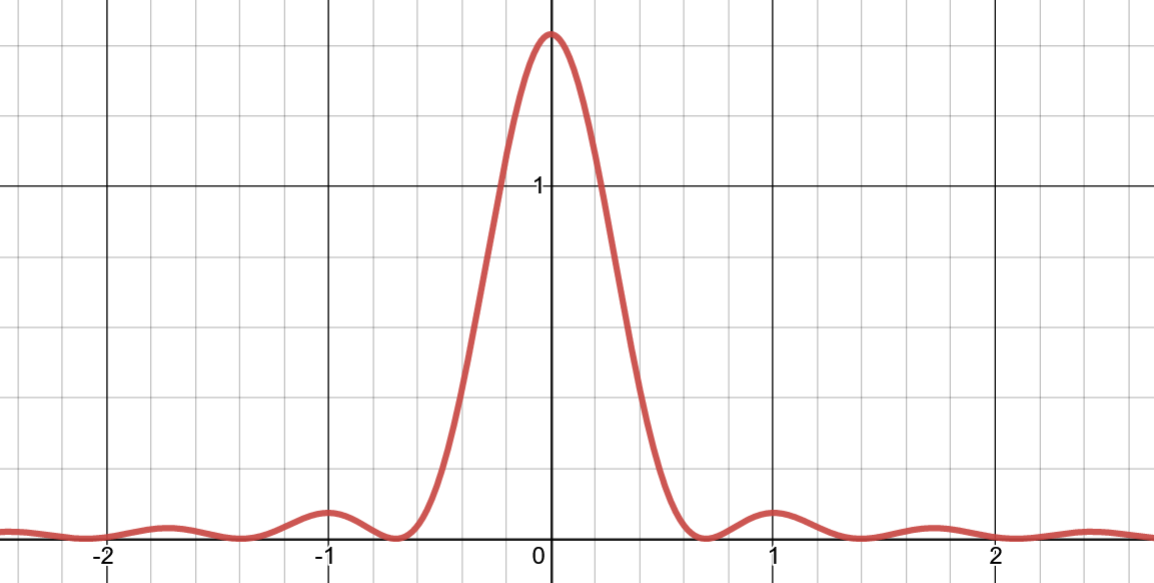
\includegraphics[width=8cm]{pictures/fejer.PNG}}

The reason we might believe that these Cesaro means converge to $f$ is that 
\[
    \sigma_N f(x) = \int_{-\pi}^\pi K_N(x-t) f(t) dt,
\]
and $K_N$ is very sharply peaked around $t = x$, so as $N$ gets larger and larger, the main contribution to the integral comes from $f(x) \approx f(t)$ if $f$ is well-behaved enough. So then we end up with 
\[
    \approx f(x) \int_{-\pi}^{\pi} K_N(x-t) dt = f(x) \cdot 1,
\]
since $k_N$ evaluates to the same over any interval of length $2\pi$ by periodicity. So that's a heuristic motivation for working with the Cesaro means here! (Some of these properties also applied when we did a similar procedure with our partial sums $S_Nf(x)$, but the \textbf{Dirichlet kernel is not nonnegative} -- that difference actually makes a big difference in the final proof.)

\begin{proof}
Recall that 
\[
    S_kf(x) = \int_{-\pi}^{\pi} D_k(x-t) f(t) dt
\]
for the Dirichlet kernel 
\[
    D_k(t) = \begin{cases} \frac{2N+1}{2\pi} & t = 0 \\ \frac{1}{2\pi} \frac{\sin\left(\left(N + \frac{1}{2}\right)t\right)}{\sin \frac{t}{2}} & \text{otherwise}. \end{cases}
\]
We can use this fact to find that 
\[
    \sigma_Nf(x) = \frac{1}{N+1} \sum_{k=0}^N S_kf(x) = \int_{-\pi}^{\pi} \frac{1}{N+1} \sum_{k=0}^N D_k(x-t) f(t) dt,
\]
and thus we know that the desired kernel is
\[
    K_N(x-t) = \frac{1}{N+1}\sum_{k=0}^N D_k(x-t).
\]
We can now substitute in our expression for $D_k$, using the variable $x$ instead of $x-t$. The case $x = 0$ can be done easily (we just have constants), and for all other $x$ we can slightly rewrite our expression as
\[
    K_N(x) = \frac{1}{2\pi(N+1)} \frac{1}{2\left(\sin \frac{x}{2}\right)^2} \sum_{k=0}^N 2\sin \frac{x}{2} \sin \left(\left(k + \frac12\right)x\right).
\]
By the trig product-to-sum identity, this simplifies to 
\[
    =  \frac{1}{2\pi(N+1)} \frac{1}{2\left(\sin \frac{x}{2}\right)^2} \sum_{k=0}^N \cos (kx) - \cos \left((k+1)x\right),
\]
and this is a telescoping sum which simplifies to 
\[
    = \frac{1}{2\pi(N+1)} \frac{1}{2\left(\sin \frac{x}{2}\right)^2} \left(1 - \cos((N+1)x)\right).
\]
We can now use another trig formula $\frac{1 - \cos x}{2} = \cos^2\left(\frac{x}{2}\right)$ to get 
\[
    =  \frac{1}{2\pi(N+1)} \frac{1}{\left(\sin \frac{x}{2}\right)^2} \sin^2\left(\frac{N+1}{2}x\right),
\]
which is indeed the expression for our Fej\'er kernel.

We can now verify the properties of the Fej\'er kernel directly: \textbf{(1)} is true because we have a manifestly positive expression and $\sin^2(cx)$ is even, and \textbf{(2)} is true because $\sin^2$ is also periodic with half the period of the corresponding $\sin$. For \textbf{(3)}, notice that 
\[
    \int_{-\pi}^\pi D_k(t) dt = \int_{-\pi}^\pi \sum_{n=-k}^k e^{int} dt,
\]
and the integral of $e^{int}$ is zero unless $n = 0$ (by $2\pi$-periodicity), so we just pick up the $n = 0$ term and get $1$. Since $\sigma_N$ is the average of the $D_k$s, the integral of $\sigma_N$ is also the average of the average of the $D_k$s, which will also be $1$.  

Finally, for \textbf{(4)}, notice that $\sin^2\frac{x}{2}$ is an even function which is increasing on $[0, \pi]$. So if we pick some $\delta \in (0, \pi)$, we can say that 
\[
    \delta \le |x| \le \pi \implies \sin^2\frac{x}{2} \ge \sin^2\frac{\delta}{2},
\]
so we indeed get the expected
\[
    K_N(x) = |K_N(x)| \le \frac{1}{2\pi(N+1) \sin^2\frac{\delta}{2}} \sin^2 \left(\frac{N+1}{2} x\right) \le \frac{1}{2\pi(N+1) \sin^2\frac{\delta}{2}}.
\]
\end{proof}

Now, we can prove convergence of the Cesaro means $\sigma_N f$ to $f$ by first doing it for continuous functions -- we showed that the continuous functions with endpoints $0$ are dense in $L^2$ (so we can show convergence appropriately), and continuous functions with endpoints both $0$ can indeed be treated as $2\pi$-periodic. So the subspace of $2\pi$-periodic continuous functions is dense in $L^2$, and we'll consider this dense subset first because it's where the heuristic argument we made above applies rigorously.

\begin{theorem}[Fej\'er]
Let $f \in C([-\pi, \pi])$ be $2\pi$-periodic (so $f(-\pi) = f(\pi)$). Then $\sigma_N f \to f$ uniformly on $[-\pi, \pi]$.
\end{theorem}

In other words, we have an even stronger result than $L^2$ convergence, now that we're limiting ourselves to continuous functions and have the stronger uniform norm. But this does \textbf{not} imply that the Fourier series of $f$ converges pointwise to $f$ -- there are indeed Fourier series representations of continuous functions that diverge at a point. Instead, it's the Cesaro mean and the Fej\'er kernel that help us out here!

\begin{proof}
First, we extend $f$ to all of $\RR$ by periodicity (defining it so that $f(x + 2\pi) = f(x)$ for all $x \in \RR$). Our function is then an element of $C(\RR)$ (still continuous), and it is $2\pi$-periodic, so it is uniformly continuous and bounded on all of $\RR$ (that is, $||f||_{\infty} = \sup_{x \in [-\pi, \pi]} f(x) < \infty$). 

We wish to show that $\sigma_N f$ converge uniformly on $f$, which means that for all $\eps > 0$ we need to find an $M$ so that for all $n \ge M$, we have $|\sigma_N f(x) - f(x)| < \eps$ for all $x$. Indeed, for any $\eps > 0$, by uniform continuity of $f$, there exists some $\delta > 0$ so that for all $|y-z| < \delta$, we have $|f(y) - f(z)| < \frac{\eps}{2}$. So now we can choose $M \in \NN$ so that for all $N \ge M$, we have
\[
    \frac{2||f||_{\infty}}{(N+1) \sin^2\frac{\delta}{2}} < \frac{\eps}{2}.
\]
(we can do this because the left-hand side converges to $0$ as $N \to \infty$). Now because $f$ and $K_N$ are $2\pi$-periodic, we can write the Cesaro mean as 
\[
    \sigma_N f(x) = \int_{-\pi}^{\pi} K_N(x-t) f(t) dt = \int_{x-\pi}^{x+\pi} K_N(\tau) f(x-\tau) d\tau
\]
by a change of variables (which is allowed because we're doing integrals over continuous functions, and thus we can use the Riemann integral), and now we have the product of $2\pi$-periodic functions, so the integral of that is the same over any interval of length $2\pi$: switching back to $t$ from $\tau$,
\[
    = \int_{-\pi}^{\pi} K_N(t) f(x-t) dt.
\]
We can now say that for all $N \ge M$ and for all $x \in [\pi, \pi]$, we have
\[
    |\sigma_N f(x) - f(x)| = \left|\int_{-\pi}^{\pi} K_N(t) f(x-t) dt - \int_{-\pi}^{\pi} K_N(t) f(x) dt\right|
\]
where we've added in a $\int_{-\pi}^{\pi} K_N(t) dt$ integral to the $f(x)$ term, which is okay because $f(x)$ doesn't talk to the $t$-integral. Combining the integrals by linearity gives us 
\[
    = \left|\int_{-\pi}^{\pi} K_N(t) \left(f(x-t) - f(x)\right) dt\right|.
\]
We'll use the triangle inequality and then split this integral into two parts now:
\[
    \le \int_{-\pi}^{\pi} \left| K_N(t) \left(f(x-t) - f(x)\right) \right| dt = \int_{|t| \le \delta} K_N(t) \left|f(x-t) - f(x)\right| dt + \int_{\delta \le |t| \le \pi} K_N(t) \left|f(x-t) - f(x)\right| dt
\]
(also using the fact that $K_N$ is always nonnegative). And now we can use our bounds above to simplify this: for the first term, we know that $|(x-t) - x| < \delta$ over the bounds of integration, so $|f(x-t) - f(x)| < \frac{\eps}{2}$. And for the second term, we know that $|f(x-t) - f(x)| < 2||f||_{\infty}$ because both $f(x-t)$ and $f(x)$ have magnitude at most $||f||_{\infty}$ for a continuous function, and when $|t| > \delta$ we can use condition \textbf{(4)} of the Fej\'er kernel. Putting this all together, we find the inequality
\[
    < \frac{\eps}{2}\int_{|t| \le \delta} K_N(t) dt + \frac{2||f||_\infty}{2\pi(N+1) \sin^2\frac{\delta}{2}} \int_{\delta \le |t| \le \pi} K_N(t) dt.
\]
We can now bound both integrals here by the integral over the entire region to get 
\[
    \le \frac{\eps}{2} + \frac{2||f||_{\infty}}{(N+1) \sin^2\frac{\delta}{2}} < \frac{\eps}{2} + \frac{\eps}{2} = \eps
\]
by our choice of $N$. So we've indeed shown uniform convergence -- $\sigma_N f$ is eventually close enough to $f$ for large enough $N$ -- and we're done. 
\end{proof}

\begin{remark}
This same proof can be modified if instead of knowing that $K_n(x) \ge 0$ (which we know for the Fej\'er kernel), we have that
\[
    \sup_N \int_{-\pi}^{\pi} |K_N(x)| < \infty.
\]
Then we can show the same uniform convergence by modifying our proof above. But if we try to plug in our Dirichlet kernel here, the condition is not satisfied, since 
\[
    \int_{-\pi}^{\pi} |D_N(x)| dx \sim \log N.
\]
So having ``almost all of the properties'' isn't enough for us to get the analogous results for the Dirichlet kernel!
\end{remark}

Now that we've proven that the Cesaro means of a continuous function converge uniformly to that function, we want to show that the Cesaro means of an $L^2$ function converge to an $L^2$ function, which would show the condition on the Hilbert space that we want and show convergence of the Fourier series as well. We'll first need the following result:

\begin{proposition}\label{cesaroineq}
For all $f \in L^2([-\pi, \pi])$, we have $||\sigma_N f||_2 \le ||f||_2$.
\end{proposition}
\begin{proof}
We'll first do this for $2\pi$-periodic functions. First suppose that $f \in C([-\pi, \pi])$ is $2\pi$-periodic -- extend $f$ to all of $\RR$ as before, and then the Cesaro mean is $\sigma_Nf(x) = \int_{-\pi}^{\pi} f(x-t) K_N(t) dt$. Thus, we can write out
\[
    \boxed{||\sigma_Nf||_2^2} = \int_{-\pi}^{\pi} |\sigma_Nf(x)|^2 dx = \int_{-\pi}^\pi \int_{-\pi}^\pi \int_{-\pi}^\pi f(x-s) \overline{f(x-t)} K_N(s) K_N(t) ds dt dx.
\]
All of these functions are continuous, so we can change the order of integration by Fubini's theorem to get 
\[
    = \int_{-\pi}^\pi \int_{-\pi}^\pi K_N(s) K_N(t) \left[\int_{-\pi}^{\pi} f(x-s) \overline{f(x-t)} dx\right] ds dt.
\]
By Cauchy-Schwarz, this can be bounded by 
\[
    \le \int_{-\pi}^\pi \int_{-\pi}^\pi K_N(s) K_N(t) ||f(\cdot -s)||_2 ||f(\cdot-t)||_2 ds dt,
\]
where $f(\cdot-s)$ denotes the function that maps $x \mapsto f(x-s)$. And now we're integrating a periodic function $f(\cdot -s)$ over an interval of length $2\pi$, so we can replace that expression with $||f||_2$ (just shifting to another length $2\pi$ interval). Doing the same with $f(\cdot -t)$ gives us
\[
    = ||f||_2^2\int_{-\pi}^\pi \int_{-\pi}^\pi K_N(s) K_N(t)  ds dt = \boxed{||f||_2^2},
\]
because the integral of $K_N$ is $1$. This gives us the desired inequality for $2\pi$-periodic functions, and now to extend it to all functions in $L^2$, suppose we have some general $f \in L^2$. From exercises, we know that there exists a sequence $\{f_n\}_n$ of $2\pi$-periodic continuous functions that converge to $f$ in $L^2$, meaning that $||f_n - f||_2 \to 0$. So from the definition of the Cesaro means, this means that $||\sigma_N f_n - \sigma_N f||_2 \to 0$ for any fixed $N$ and as $N \to \infty$, leading us to 
\[
    ||\sigma_N f||_2 = \lim_{n \to \infty} ||\sigma_N f_n||_2 \le \lim_{n \to \infty} ||f_n||_2
\]
(using the $2\pi$-periodic case), and this last result is $||f||_2$ because $f_n$ converges to $f$ in $L^2$.
\end{proof}

So now we're almost done, and combining the two results above will give us what we want:

\begin{theorem}
For all $f \in L^2$, $||\sigma_N f - f||_2 \to 0$ as $N \to \infty$. Therefore, if $\hat{f}(n) = 0$ for all $n$, then $f = 0$ (since $\sigma_N f = 0$ for all $N$).
\end{theorem}
\begin{proof}
(We only need to prove the result in the first sentence -- the second follows directly as stated.) Let $f \in L^2([-\pi, \pi])$, and let $\eps > 0$. By density of the $2\pi$-periodic continuous functions, there exists some $2\pi$-periodic $g \in C([-\pi, \pi])$ so that $||f-g||_2 < \frac{\eps}{3}$. Because $\sigma_N g \to g$ uniformly on $[-\pi, \pi]$, there exists some $M$ so that for all $N \ge M$ and for all $x \in [-\pi, \pi]$, we have $|\sigma_Ng(x) - g(x)| < \frac{\eps}{3\sqrt{2\pi}}$.  

Now for all $N \ge M$, the triangle inequality tells us that
\[
    ||\sigma_Nf - f||_2 \le ||\sigma_N f - \sigma_N g||_2 + ||\sigma_N g - g||_2 + ||g - f||_2.
\]
The first term is $||\sigma_N(f-g)||_2$ (we can check this from the definition), and by \cref{cesaroineq}, that is less than $||f-g||_2 < \frac{\eps}{3}$. Meanwhile, the last term is also bounded by $\frac{\eps}{3}$, and the middle term is $\left(\int_{-\pi}^{\pi} |\sigma_N g(x) - g(x) |^2 dx \right)^{1/2} < \left(2\pi \cdot\left(\frac{\eps}{3\sqrt{2\pi}}\right)^2\right)^{1/2} = \frac{\eps}{3}$. So putting this all back into our expression gives us
\[
     ||\sigma_Nf - f||_2 < \frac{\eps}{3} + \frac{\eps}{3} + \frac{\eps}{3} = \eps,
\]
completing the proof.
\end{proof}

So we've now seen a concrete application of the general machinery we've built up for Hilbert spaces! In summary, we've shown that the normalized exponentials form a maximal orthonormal set, so that the partial Fourier sums of $f$ converge to $f$ in $L^2$. But as previous mentioned, we don't have pointwise convergence everywhere -- instead, we can only say that there is a \textbf{subsequence} that converges to $f$ pointwise. And in fact, \textbf{Carleson's theorem }is a deep result in analysis that tells us that for all $f \in L^2$, $S_Nf(x) \to f(x)$ \textbf{almost everywhere}.

We can also ask questions about the convergence of Fourier series in other $L^p$ spaces, since all of the definitions also make sense there. It is known additionally that for all $1 < p < \infty$, we always have $||S_N f - f||_p \to 0$, and that this is false for $p = 1, \infty$. But deeper harmonic analysis is needed to prove statements like this, and in particular we would need to learn how to work with \textbf{singular integral operators}.

In this class, though, this is as far as we'll go with Fourier series, and next time, we'll move on to the topic of \textbf{minimizers over closed convex sets} and (as a consequence) how to identify the dual of a Hilbert space with the Hilbert space itself in a canonical way. 

\pagebreak\section*{April 22, 2021}

Last time, we discussed orthonormal bases, considering the concrete question of whether complex exponentials formed an orthonormal basis for $L^2([-\pi, \pi])$. Today, we'll go back to a general discussion of Hilbert spaces, and the rest of the course from here on will be general theory and some concrete applications to particular problems. 

Our first topic today will be \textbf{length minimizers}: recall that we can describe a norm on $V/W$ for subspaces of a normed vector space, and we did so via an infimum. It makes sense to ask whether this minimal distance is actually achieved:

\begin{theorem}\label{lengthminimizer}
Let $C$ be a nonempty closed subset of a Hilbert space $H$ which is \vocab{convex}, meaning that for all $v_1, v_2 \in C$, we have $tv_1 + (1-t)v_2 \in C$ for all $t \in [0, 1]$. Then there exists a unique element $v \in C$ with $||v|| = \inf_{u \in C} ||u||$ (this is a length minimizer).
\end{theorem}

The convexity condition can alternatively be stated as ``the line segment between any two elements of $C$ is contained in $C$.'' And to connect this with our discussion earlier, one such example of a set would be $v + W$ for some closed subspace $W$ of $C$ and some $v \in H$. 

\begin{remark}
The condition that $C$ is closed is required: for example, we can let $C$ be an open disk outside the origin, in which case the minimum norm is not achieved (because it's on the boundary). And convexity is also required -- for example, otherwise we could take the complement of an open disk centered at the origin, in which case the minimum norm is achieved on the entire boundary. 
\end{remark} 

\begin{proof}
We should recall that $a = \inf S$ if and only if $a$ is a lower bound for $S$, and there exists a sequence $\{s_n\}$ in $S$ with $s_n \to a$. If we let $d = \inf_{u \in C} ||u||$, this is some finite number because norms are always bounded from below by $0$, and $C$ is nonempty. So there exists some sequence $\{u_n\}$ in $C$ such that $||u_n|| \to d$. 

We claim that this sequence is actually Cauchy. To see that, let $\eps > 0$ -- because of convergence of $||u_n||$ to $d$, there exists some $N$ so that for all $n \ge N$, we have 
\[
    2||u_n||^2 < 2d^2 + \frac{\eps^2}{2}.
\] 
Then for all $n, m \ge N$, the parallelogram law tells us that
\[
    ||u_m - u_n||^2 = 2||u_m||^2 + 2||u_n||^2 - 4\left|\left|\frac{u_n + u_m}{2}\right|\right|^2,
\]
and now because $\frac{u_n + u_m}{2}$ lies on the line segment between $u_n$ and $u_m$ (taking $t = \frac{1}{2}$), convexity tells us that it is also in $C$. Therefore, $\left|\left|\frac{u_n + u_m}{2}\right|\right|^2 \ge d^2$, and thus
\[
    ||u_m - u_n||^2 \le 2||u_m||^2 - 2d^2 + 2||u_n||^2 - 2d^2 < \frac{\eps^2}{2} + \frac{\eps^2}{2} = \eps^2
\]
by our choice of $N$, and taking a square root shows that the sequence $\{u_n\}$ is indeed Cauchy. Because our Hilbert space is complete, this means that the sequence also converges, and thus there is some $v \in H$ such that $u_n \to v$, and $v \in C$ as well because our subset $C$ is closed. So now continuity of the norm tells us that
\[
    ||v|| = \lim_{n \to \infty} ||u_n|| = d,
\]
and thus we've found our minimizer $v \in C$. To show uniqueness, suppose that $v, \overline{v}$ are both in $C$ and have norm $d$. Then the parallelogram law tells us that
\[
    ||v - \overline{v}||^2 = 2||v||^2 + 2||\overline{v}||^2 - 4\left|\left|\frac{v + \overline{v}}{2}\right|\right|^2 \le 2d^2 + 2d^2 - 4d^2 = 0,
\]
again using that $\frac{v + \overline{v}}{2}$ is also in $C$ by convexity, and thus we must have $v - \overline{v} = 0 \implies v = \overline{v}$.
\end{proof}

We'll obtain some important consequences from this result -- the first one is how to decompose our Hilbert space using a closed linear subspace, much like we usually like to do in $\RR^n$ and $\CC^n$.

\begin{theorem}\label{orthocomplement}
Let $H$ be a Hilbert space, and let $W \subset H$ be a subspace. Then the \vocab{orthogonal complement}
\[
    W^\perp = \{u \in H: \langle u, w \rangle = 0 \quad \forall w \in W\}
\]
is a closed linear subspace of $H$. Furthermore, if $W$ is closed, then $H = W \oplus W^\perp$; in other words, for all $u \in H$, we can write $u = w + w^\perp$ for some unique $w \in W$ and $w^\perp \in W^\perp$.)
\end{theorem}

A picture to keep in mind is the case where $H$ is $\RR^2$ and $W$ is the $x$-axis -- then $W^\perp$ would be the $y$-axis, and we're saying that all elements can be broken up into a component along the $x$-axis and a component along the $y$-axis.

\begin{proof}
Showing that $W^\perp$ is a subspace is clear, because if $\langle u_1, w \rangle = 0$ and $\langle u_2,  w\rangle = 0$ for all $w \in W$, any linear combination of $u_1$ and $u_2$ will also be orthogonal to all $w \in W$ by linearity of the inner product. Furthermore, $W \cap W^\perp = \{0\}$, because any element $w \in W$ that is also in $W^\perp$ must satisfy $\langle w, w \rangle = 0 \implies w = 0$. 

To show that $W^\perp$ is closed, let $\{u_n\}$ be a sequence in $W^\perp$ converging to $u \in H$. We wish to show that $\langle u, w \rangle = 0$ for all $w \in W$, so that $u \in W^\perp$ as well. Indeed, by continuity of the inner product, we have
\[
    \langle u, w \rangle = \lim_{n \to \infty} \langle u_n, w \rangle = \lim_{n \to \infty} 0 = 0,
\]
so that our sequential limit is also in our subspace $W^\perp$. 

It remains to show that $H = W \oplus W^\perp$ if $W$ is closed. The result is clear for $W = H$, since $W^\perp = \{0\}$ and $H = H \oplus \{0\}$ is a trivial decomposition. Otherwise, if $W \ne H$, then let $u \in H \setminus W$ (that is, $u$ is in $H$ but not $W$), and define the set 
\[
    C = u + W = \{u + w: w \in W\}.
\]
This set $C$ is nonempty because it contains $u$, and it is convex because for any two elements $u + w_1, u + w_2 \in C$ (for $w_1, w_2 \in W$) and for any $t \in [0, 1]$, we have
\[
    t(u + w_1) + (1-t) (u + w_2) = (t + (1-t)) u + tw_1 + (1-t) w_2 = u + \left(tw_1 + (1-t) w_2\right)
\]
and the last term is in $W$ because subspaces are closed under linear combinations. So we now need to show that $C$ is closed: indeed, if $u + w_n$ is a sequence of elements in $C$ that converge to some element $v \in H$, we know that 
\[
    u + w_n \to v \implies w_n \to v- u,
\]
and because $W$ is closed, $w_n$ must converge to some element in $W$. Thus $v - u \in W$, and thus $v = u + w$ for some $w \in W$, which is exactly the definition of being in $C$. So $C$ is indeed closed.

So returning to the problem, if we want to write an element $u$ of $H$ as a sum of a part in $W$ and a part in $W^\perp$, it makes sense that our component in $W^\perp$ will be the minimizer to $C$ (keeping the $\RR^2$ example from above in mind). So applying \cref{lengthminimizer}, because $C$ is closed and convex, there is some unique $v \in C$ with 
\[
    ||v|| = \inf_{c \in C} ||c|| = \inf_{w \in W} ||u + w||.
\].
Since $v \in C$, we know that $u - v \in W$, so we will write $u = (u-v) + v$. Our goal is to show that $v \in W^\perp$, and we do this with a variational argument (in physics, this is the Euler-Lagrange equations, and it is another way of phrasing properties of the infimum). If $w \in W$, define the function 
\[
    f(t) = ||v + tw||^2 = ||v||^2 + t^2 ||w||^2 + 2t \text{Re}\langle v, w \rangle,
\]
which is a polynomial in $t$. We know that $f(t)$ has a minimum at $t = 0$, because all elements of the form $v + tw$ are in $C$, and we know the minimizer of norm uniquely occurs at $v$. So $f'(0) = 0$, and thus
\[
    2 \text{Re}\langle v, w \rangle = 0.
\]
So the real part of the inner product is zero, and now we can repeat this argument but with $||v + itw||$ instead of $||v + tw||$, which will show us that 
\[
    \text{Re}\langle v, iw \rangle = \text{Im}\langle v, w \rangle = 0. 
\]
Therefore, $\langle v, w \rangle = 0$, and since this argument was true for all $w \in W$, we must have $v \in W^\perp$. It remains to show that this decomposition is unique, and this is true because $W \cap W^\perp = \{0\}$: more specifically, if $u = w_1 + w_1^\perp = w_2 + w_2^\perp$, that means that $w_1 - w_2 = w_2^\perp - w_1^\perp$ is in both $W$ and $W^\perp$, and thus both sides of this equation are $0$. So $w_1 = w_2$ and $w_1^\perp = w_2^\perp$, showing uniqueness.
\end{proof}

The following result is left as an exercise for us:

\begin{theorem}
If $W \subset H$ is a subspace, then $(W^\perp)^\perp$ is the closure $\overline{W}$ of $W$. In particular, if $W$ is closed, then $(W^\perp)^\perp = W$.
\end{theorem}

Now that we have this decomposition $u = w + w^\perp$ for our subspace $W$, we can construct a map which takes in $u$ and outputs $w$. If we use the $\RR^2$ example from above, we can see that this map is a projection onto the $x$-axis, and more generally we can make the following definition:

\begin{definition}
Let $P: H \to H$ be a bounded linear operator. Then $P$ is a \vocab{projection} if $P^2 = P$.
\end{definition}

\begin{proposition}
Let $H$ be a Hilbert space, and let $W \subset H$ be a closed subspace. Then the map $\Pi_W: H \to H$ sending $v = w + w^\perp$ (for $w \in W, w^\perp = W^\perp$) to $w$ is a projection operator.
\end{proposition}
\begin{proof}
First, we show that $\Pi_W$ is linear. Indeed, if $v_1 = w_1 + w_1^\perp$ and $v_2 = w_2 + w_2^\perp$, and we have $\lambda_1, \lambda_2 \in \CC$, then 
\[
    \lambda_1 v_1 + \lambda_2 v_2 = (\lambda_1 w_1 + \lambda_2 w_2) + (\lambda_1 w_1^\perp + \lambda_2 w_2^\perp).
\]
The two terms on the right-hand side are in $W$ and $W^\perp$, respectively, by closure of subspaces under linear combinations. So $\Pi_W(\lambda_1 v_1 + \lambda_2 v_2) = \lambda_1 w_1 + \lambda_2 w_2$, which is indeed $\lambda_1 \Pi_W(v_1) + \lambda_2 \Pi_W(v_2)$, as desired. We can also see that $\Pi_W$ is bounded, because when $v = w + w^\perp$, 
\[
    ||v||^2 = ||w + w^\perp||^2 = ||w||^2 + ||w_\perp||^2 \ge ||w||^2
\]
(since the inner product cross term is zero when $\langle w, w^\perp \rangle = 0$). Therefore, $||\Pi_W(v)|| \le ||v||$, and the operator norm is at most $1$. And now we just need to check that $\Pi_W^2 = \Pi_W$: if $v = w + w^\perp$, then $\Pi_W(v) = w$, and then 
\[
    \Pi_W(\Pi_W(v)) = \Pi_W(w) = w = \Pi_W(v),
\]
and since this is true for all $v$, we have $\Pi_W^2 = \Pi_W$, as desired.
\end{proof}

Our next application of length minimizers will be the following important result:

\begin{theorem}[Riesz Representation Theorem]
Let $H$ be a Hilbert space. Then for all $f \in H'$, there exists a unique $v \in H$ so that $f(u) = \langle u, v \rangle$ for all $u \in H$. 
\end{theorem}

In other words, every element of the dual can be realized as an inner product with a fixed vector. We've seen something similar before when we proved that the dual of $\ell^p$ is identified with $\ell^q$ (for $\frac{1}{p} + \frac{1}{q} = 2$) via a pairing, and the $p = q = 2$ case is the example relevant to Hilbert spaces.

\begin{proof}
If such a $v$ exists, it is unique, because $f(u) = \langle u, v \rangle = \langle u, \tilde{v} \rangle = 0$, then $\langle u, v - \overline{v} \rangle = 0$ for all $u \in H$. Setting $u = v - \overline{v}$ tells us that $v - \overline{v} = 0$. So we just need to construct such a $v$ that works.

The easiest case is $f = 0$, because in that case, we take $v = 0$. Otherwise, there exists some $u_1 \in H$ so that $f(u_1) \ne 0$, and we take $u_0 = \frac{u_1}{f(u_1)}$ so that $f(u_0) = 1$. We can then define the nonempty set
\[
    C = \{u \in H: f(u) = 1\} = f^{-1}(\{1\}),
\] 
which is closed because $f$ is a continuous function, $\{1\}$ only has one element so is closed, and the preimage of a closed set by a continuous function is a closed set. We claim that $C$ is convex: indeed, if $u_1, u_2 \in C$ and $t \in [0, 1]$, then 
\[
    f(tu_1 + (1-t) u_2) = t f(u_1) + (1-t) f(u_2) = t \cdot 1 + (1-t) \cdot 1 = 1,
\]
so that $tu_1 + (1-t)u_2$ is also in $C$. So now by \cref{lengthminimizer}, there exists $v_0 \in C$ so that $v_0 = \inf_{u \in C} ||u||$, and we define $v = \frac{v_0}{||v_0||^2}$ (noting that $v_0 \ne 0$ because the infimum is not $0$). 

We claim that this is the $v$ that we want; in other words, let's check that $f(u) = \langle u, v \rangle$. Indeed, if we let $N = f^{-1}(\{0\}) = \{w \in H: f(w) = 0\}$ be the nullspace of $f$, then we can check that $C = \{v_0 + w: w \in N\}$ and that $||v_0|| = \inf_{w \in N} ||v_0 + w||$. So by the argument that we made earlier in \cref{orthocomplement} using $||v_0 + tw||^2$, $v_0 \in N^\perp$, and now for any $w \in H$,
\[
    f(u - f(u) v_0) = f(u) - f(u) f(v_0) = 0
\]
by linearity of $f$, and thus $u = (u - f(u) v_0) + f(u)v_0$ is a sum of a component in $N$ and a component in $N^\perp$. 
\[
    \langle u, v \rangle = \frac{1}{||v_0||^2} \langle u, v_0 \rangle = \frac{1}{||v_0||^2} \left[\langle (u - f(u) v_0), v_0 \rangle + f(u) \langle v_0, v_0 \rangle\right],
\]  
The first term here has $u - f(u) v_0 \in N$ and $v_0 \in N^\perp$, so that inner product is zero, and we're left with 
\[
    = f(u) \frac{\langle v_0, v_0 \rangle}{||v_0||^2} = f(u),
\]
as desired. So we've found $v$ (a scaled version of the minimizer) so that $f(u) = \langle u, v \rangle$ for all $u$, concluding the proof.
\end{proof}

We'll study adjoint operators next time -- we defined it as a map from dual spaces to dual spaces, but because we can identify dual spaces of Hilbert spaces with themselves, adjoint operators will be essentially regular operators, and we'll soon see how they relate to solving equations on Hilbert spaces and why they are the analogs of the transpose matrix in finite-dimensional linear algebra as well.

\pagebreak\section{April 27, 2021}

We discussed the Riesz representation theorem last time, which states that for a Hilbert space $H$, we can identify each $f \in H' = \mc{B}(H, \CC)$ with a unique element $v \in H$ such that $f(u) = \langle u, v \rangle$ for all $u \in H$. (In other words, every continuous linear functional on $H$ can be realized as an inner product with a fixed vector.) 

We can use this to expand on a concept we've touched on previously in an assignment:

\begin{theorem}
Let $H$ be a Hilbert space, and let $A: H \to H$ be a bounded linear operator. Then there exists a unique bounded linear operator $A^\ast: H \to H$, known as the \vocab{adjoint} of $A$, satisfying 
\[
    \langle Au, v \rangle = \langle u, A^\ast v \rangle
\]
for all $u, v \in H$. In addition, we have that $||A^\ast|| = ||A||$.
\end{theorem}
\begin{proof}
We can show uniqueness similarly to how we showed it in the Riesz representation theorem: if $\langle u, A_1^\ast v \rangle= \langle u, A_2^\ast v \rangle$ for all $u, v$ for two potential candidates $A_1, A_2$, then $\langle u, (A_1^\ast v - A_2^\ast v) \rangle = 0$ for all $u, v$, and we can always set $u = (A_1^\ast v - A_2^\ast v)$ to show that we must have $A_1^\ast v = A_2^\ast v$ for all $v$, meaning that $A_1^\ast$ and $A_2^\ast$ were the same operator to begin with.

To show that such an operator does exist, first fix $v \in H$, and define a map $f_v: H \to \CC$ by $f_v(u) = \langle Au, v \rangle$. This is a linear map (in the argument $u$) because for any $u_1, u_2 \in H$ and $\lambda_1, \lambda_2 \in \CC$, we have
\[
    f_v(\lambda_1 u_1 + \lambda_2 u_2) = \langle A(\lambda_1 u_1 + \lambda_2 u_2), v \rangle = \langle \lambda_1 Au_1 + \lambda_2 Au_2, v \rangle
\]
by linearity of $A$, and then this simplifies to 
\[
    = \lambda_1 \langle Au_1, v \rangle + \lambda_2 \langle Au_2, v \rangle = \lambda_1 f_v(u_1) + \lambda_2 f_v(u_2)
\]  
by linearity in the first argument of the inner product. We claim this is also a continuous linear operator (so that it is actually an element of the dual). Indeed, we can check that if $||u|| = 1$, 
\[
    |f_v(u)| = |\langle Au, v \rangle| \le ||Au|| \cdot ||v||
\]
by the Cauchy-Schwarz inequality, and this is bounded by $||A|| \cdot ||v||$. Therefore, $||f_v|| \le ||A|| \cdot ||v||$ (which is a constant), and thus $f_v \in H'$. By the Riesz representation theorem, we can therefore find a (unique) element, which we denote $A^\ast v$, of $H$ satisfying
\[
    \langle Au, v \rangle = f_v(u) = \langle u, A^\ast v \rangle.
\]
We now need to show that $A^\ast$ is a bounded linear operator. For linearity, let $v_1, v_2 \in H$ and let $\lambda_1, \lambda_2 \in \CC$. We know that for all $u \in H$, 
\[
    \boxed{\langle u, A^\ast(\lambda_1 v_1 + \lambda_2 v_2) \rangle} = \langle Au, \lambda_1 v_1 + \lambda_2 v_2 \rangle,
\]
and now by conjugate linearity in the second variable, this simplifies to 
\[
    = \overline{\lambda}_1 \langle Au, v_1 \rangle + \overline{\lambda}_2 \langle Au, v_2 \rangle = \overline{\lambda}_1 \langle u, A^\ast v_1 \rangle + \overline{\lambda}_2 \langle u, A^\ast v_2 \rangle.
\]
Pulling the complex numbers back in shows that this is 
\[
    = \boxed{\langle u, \lambda_1 A^\ast v_1 + \lambda_2 A^\ast v_2 \rangle}.
\]
The only way for these two boxed expressions to be equal for all $u$ is if the two operators are equal: $A^\ast(\lambda_1 v_1 + \lambda_2v_2) = \lambda_1 A^\ast(v_1) + \lambda_2 A^\ast(v_2)$, which is the desired linearity result for $A^\ast$.

We now show that $A^\ast$ is bounded with $||A^\ast|| = ||A||$. Take a unit-norm vector $||v|| = 1$: if $A^\ast v = 0$, then clearly $||A^\ast v || \le ||A||$. Otherwise, we still want to show that same inequality. Suppose $A^\ast v \ne 0$. Then 
\[
    \boxed{||A^\ast v ||^2} = \langle A^\ast v, A^\ast v \rangle = \langle A A^\ast v, v \rangle
\]
by definition of the adjoint, and now by Cauchy-Schwarz this is bounded by 
\[
    \le ||AA^\ast v || \cdot ||v|| = ||A A^\ast v || \le \boxed{||A|| \cdot ||A^\ast v||}.
\]
Dividing by the nonzero constant $||A^\ast v||$ yields $||A^\ast v|| \le ||A||$, as desired, and now taking the sup over all $v$ with $||v|| = 1$ yields $||A^\ast|| \le ||A||$.

To finish, we need to show equality. For all $u, v \in H$, we have
\[
    \langle A^\ast u, v \rangle = \overline{\langle v, A^\ast u \rangle} = \overline{\langle Av, u \rangle} = \langle u, Av \rangle,
\]
so the adjoint of the adjoint of $A$ is $A$ itself (since $\langle u, Av \rangle = \langle A^\ast u, v \rangle = \langle u, (A^\ast)^\ast v \rangle$). Therefore, we can flip the roles of $A^\ast$ and $A$ in this argument to find that
\[
    ||(A^\ast)^\ast|| \le ||A^\ast|| \implies ||A|| \le ||A^\ast||,
\]
and putting the inequalities together yields $||A|| = ||A^\ast||$ as desired. 
\end{proof}

Let's see a concrete example of what these adjoint operators look like:

\begin{example}
If our Hilbert space is $H = \CC^n$, so that $u$ is an $n$-dimensional vector, then we know that 
\[
    (Au)_i = \sum_{j=1}^n A_{ij} u_j
\]
for some fixed complex numbers $A_{ij}$, and we can represent $A$ as a finite-dimensional matrix.
\end{example}

To determine the adjoint of $A$, we need to figure out the operator $B$ that satisfies $\langle Au, v \rangle = \langle u, Bv \rangle$. Towards that, notice that
\[
    \langle Au, v \rangle  = \sum_{i=1}^n (Au)_i \overline{v}_i = \sum_{i,j} A_{ij} u_j \overline{v}_i 
\]
and switching the order of summation yields 
\[
    = \sum_{j=1}^n u_j \overline{\sum_{i=1}^n \overline{A}_{ij} v_i} = \sum_{j=1}^n u_j \overline{(A^\ast v)_j},
\]
where the adjoint of $A$ acts on $v$ as 
\[
    (A^\ast v)_i = \sum_{j=1}^n \overline{A_{ji}} v_j.
\]
So for matrices, the adjoint is also representable by a martix, and it is the conjugate transpose of $A$.

\begin{example}
Now consider the space $\ell^2$, in which an operator is described with a double sequence $\{A_{ij}\}^\infty$ in $\CC$ so that 
\[
    \sum_{i,j} |A_{ij}|^2 = \lim_{N \to \infty} \sum_{i=1}^N \sum_{j=1}^N |A_{ij}|^2 < \infty.
\]
\end{example}

Specifically, we define $A: \ell^2 \to \ell^2$ via
\[
    (A \underline{a})_i = \sum_{j=1}^{\infty} A_{ij} a_j.
\]
We can check by the Cauchy-Schwarz inequality that this is a bounded linear operator as long as $\sum_{i,j} |A_{ij}|^2$ is satisfied (the order of summation does not matter because all terms in the double sum are nonnegative). So $A \in \mc{B}(\ell^2, \ell^2)$, and for all $\underline{a}, \underline{b} \in \ell^2$, we have
\[
    \langle A \underline{a}, \underline{b} \rangle_{\ell^2} = \sum_i \sum_j A_{ij} a_j \overline{b}_i = \sum_j a_j \overline{\left(\sum_i \overline{A}_{ij} b_i \right)} = \langle \underline{a}, A^\ast \underline{b} \rangle,
\]
where we define the adjoint similarly to in the finite-dimensional case:
\[
    (A^\ast\underline{b})_i = \sum_{j=1}^{\infty} \overline{A}_{ji} b_j.
\]

Finally, we can try doing an integral instead of an infinite sum:

\begin{example}
Let $K \in C([0, 1] \times [0, 1])$, and define the map $A: L^2([0, 1]) \to L^2([0, 1])$ via
\[
    Af(x) = \int_0^1 K(x, y) f(y) dy.
\]
\end{example}

We can then check that the adjoint $A^\ast$ is defined as
\[
    A^\ast g(x) = \int_0^1 \overline{K(y, x)} g(y) dy,
\]
so we're again flipping the indices and taking a complex conjugate. 

\begin{theorem}
Let $H$ be a Hilbert space, and let $A: H \to H$ be a bounded linear operator. Then 
\[
    (\text{Ran}(A))^\perp = \text{Null}(A^\ast),
\]
where $\text{Ran}(A)$ is the range of $A$ (the set of all vectors of the form $Au$), and $\text{Null}(A^\ast)$ is the nullspace of $A^\ast$ (the set of all vectors for which $A^\ast u = 0$).
\end{theorem}

In particular, if we know that the range of $A$ is a closed subspace, then always being able to solve $Au = v$ (surjectivity) is equivalent to knowing that that the adjoint is one-to-one (injectivity), sine the range of $A$ is then the orthogonal complement of the zero vector, which is the whole space. 

\begin{proof}
Note that $v \in \text{Null}(A^\ast)$ if and only if $\langle u, A^\ast v \rangle = 0$ for all $u \in H$, which is equivalent to $\langle Au, v \rangle = 0$ for all $u \in H$. So $v$ is orthogonal to all elements in $\text{Ran}(A)$, and that's equivalent to saying that $v \in \text{Ran}(A)^\perp$. (All steps here go in both directions, so this shows the equivalence of the two sets.)
\end{proof}

This is essentially an infinite-dimensional version of rank-nullity, and we want to see if we can say similar things about the solutions to linear equations that we could in the finite-dimensional case (our input needs to satisfy certain linear relations, and then our final solution is unique up to a linear subspace). But before we get to that, these operators that we'll solve solvability for have particular important properties on bounded sequences. We take for granted that a bounded linear operator takes bounded sets to bounded sets in finite-dimensional spaces, and so we can find a convergent subsequence using Heine-Borel. So the point is that there is some compactness hidden in here in $\RR^n$ and $\CC^n$, so we need to study some facts about how compactness and Hilbert spaces before we can talk about solvability of equations.

\begin{definition}
Let $X$ be a metric space. A subset $K \subset X$ is \vocab{compact} if every sequence of elements in $K$ has a subsequence converging to an element of $K$. 
\end{definition}

\begin{example}
By the Pigeonhole Principle, all finite subsets are compact.
\end{example}

As just described, we also have the following result from real analysis:

\begin{theorem}[Heine-Borel]
A subset $K \subset \RR$ (also $\RR^n$ and $\CC^n$) is compact if and only if $K$ is closed and bounded.
\end{theorem}

Examples on the real line include closed intervals and also the set $\{0\} \cup \{\frac{1}{n}: n \in \NN\}$. We know this doesn't hold for arbitrary metric spaces or even Banach spaces, and in fact it's still not true for Hilbert spaces:

\begin{example}
Let $H$ be an infinite-dimensional Hilbert space. Then the closed ball 
\[
    F = \{u \in H: ||u|| \le 1\}
\]
is a closed and bounded set, but it is not compact.
\end{example}

This is because we can let $\{e_n\}_{n=1}^{\infty}$ be a countably infinite orthonormal subset of $H$ (it doesn't need to be a basis), which we find by Gram-Schmidt, so that all elements $e_n$ are in $F$, but 
\[
    ||e_n - e_k||^2 = ||e_n||^2 + ||e_k||^2 + 2 \text{Re}\langle e_n, e_k \rangle = 2.
\]
So the distance between any two elements of the sequence is $2$, so there is no convergent subsequence (since it cannot be Cauchy).

Motivated by this, we know that all compact sets are closed and bounded, and thus we want to figure out an additional condition guarantees compactness for a Hilbert space (so that we can verify compactness without using the subsequence definition). And this is in fact related to something that we can discuss in 18.100B in a different context when thinking about the space of continuous functions.

\begin{definition}
Let $H$ be a Hilbert space. A subset $K \subset H$ has \vocab{equi-small tails} with respect to a countable orthonormal subset $\{e_n\}$ if for all $\eps > 0$, there is some $n \ge N$ so that for all $v \in K$, we have
\[
    \sum_{k > N} |\langle v, e_k \rangle|^2 < \eps^2.
\]
\end{definition}

We know that the sequence for any given $v$ converges by Bessel's inequality, so that the inequality above will eventually hold for some $N$ for each $v$. But this equi-small tails requirement is a more ``uniform'' condition on the rate of convergence -- we need to be able to pick an $N$ that works for all $v \in K$ at the same time. 

\begin{example}
Any finite set $K$ has equi-small tails with respect to any countable orthonormal subset (we can take the maximum of finitely many $N$s). 
\end{example}

The motivation for this definition is that, as mentioned above, finite sets are always compact, so we should hope that this additional uniformity gives us compactness. We won't get to that result today, but here's some more motivation for why this is the correct condition to add, building on the $\{0\} \cup \{\frac{1}{n}: n \in \NN\}$ example from above:

\begin{theorem}
Let $H$ be a Hilbert space, and let $\{v_n\}_n$ be a convergent sequence with $v_n \to v$. If $\{e_k\}$ is a countable orthonormal subset, then $K = \{v_n: n \in \NN\} \cup \{v\}$ is compact, and $K$ has equi-small tails with respect to $\{e_k\}$.
\end{theorem}

\begin{proof}
Compactness will be left as an exercise for us. For equi-small tails, the idea is that for sufficiently large $n$, $v_n$ will be close to $v$, so we can use $v$ to take care of all but finitely many of the points in our sequence. Let $\eps > 0$: since $v_n \to v$, there is some $M \in \NN$ so that for all $n \ge M$, we have $||v_n - v|| < \frac{\eps}{2}$. We choose $N$ large enough so that for this fixed $v$,
\[
    \sum_{k > N} |\langle v, e_k \rangle|^2 + \max_{1 \le n \le M-1} \sum_{k > N}|\langle v_n, e_k \rangle|^2 < \frac{\eps^2}{4}.
\]
(There are only finitely many terms here, and we can choose our $N$ large enough so that it makes the $n = 1$ term smaller than $\frac{\eps^2}{8}$, the $n = 2$ term smaller than $\frac{\eps^2}{16}$, and so on.) We claim that this $N$ uniformly bounds our tails: indeed, 
\[
    \sum_{k > N} |\langle v, e_k \rangle|^2 < \frac{\eps^2}{4} < \eps^2,
\]
and for all $1 \le n \le M-1$ we also have
\[
    \sum_{k > N} |\langle v_n, e_k \rangle|^2 < \frac{\eps^2}{4} < \eps^2.
\]
So we just need to check the condition for $n \ge M$: Bessel's inequality tells us that
\[
    \left(\sum_{k > N} |\langle v_n, e_k \rangle|^2 \right)^{1/2} = \left(\sum_{k > N} |\langle v_n - v, e_k \rangle + \langle v, e_k \rangle|^2 \right)^{1/2},
\]
and this is the $\ell^2$ norm of the sum of two sequences indexed by $k$, so by the triangle inequality this is boudned by 
\[
    \le \left(\sum_{k>N}|\langle v_n - v, e_k \rangle |^2\right)^{1/2} + \left(\sum_{k>N}|\langle v, e_k \rangle |^2\right)^{1/2}.
\]
The second term is at most $\frac{\eps}{2}$, and then the first term is bounded by Bessel's inequality by $||v_n - v||$. Since we chose $N$ large enough so that that norm is less than $\frac{\eps}{2}$, we indeed have that this is bounded by 
\[
    < \frac{\eps}{2} + \frac{\eps}{2} = \eps,
\]
as desired.
\end{proof}

Next time, we'll prove that if we have a subset of a separable Hilbert space which is closed, bounded, and has equi-small tails with respect to an orthonormal basis (which we know exists), then we have compactness, and then we'll rephrase that fact in a way that doesn't involve Hilbert spaces and go from there.

\pagebreak\section*{April 29, 2021}

We'll continue discussing compactness today -- recall that a subset $K$ of a metric space $X$ is \vocab{compact} if every sequence $\{x_n\}_n$ in $K$ has a subsequence that is convergent in $K$. While being closed and bounded is equivalent to being compact in $\RR^n$, this is not true in general Hilbert spaces (for example, take the orthonormal basis vectors in $\ell^2$). So we need an additional condition -- last time, we proved that if we have a convergent sequence $\{v_n\}_n$ in $H$ converging to $v$, then the subset $K = \{v_n: n \in \NN\} \cup \{v\}$ is compact, and it has \textbf{equi-small tails} with respect to any orthonormal subset. Here, the definition is that if $\{e_k\}_k$ is a countable orthonormal subset of $H$, then for all $\eps > 0$, there exists some $N \in \NN$ such that for all $\tilde{v} \in K$ (either an element of the sequence or $v$), we have 
\[
    \sum_{k > N} |\langle \tilde{v}, e_k \rangle|^2 < \eps^2.
\]
(We know that this sum over all $k$ is bounded, and thus convergent, by Bessel's inequality for any individual $\tilde{v}$, so we can always find an $N$ that makes this work for a fixed $\tilde{v}$, but the condition requires it simultaneously for all $\tilde{v} \in K$. So we can think of ``equi-small tails'' as really meaning ``uniformly small tails.'') It turns out that this condition suffices (and is necessary) for compactness:

\begin{theorem} 
Let $H$ be a separable Hilbert space, and let $\{e_k\}_k$ be an orthonormal basis of $H$. Then a subset $K \subset H$ is compact if and only if $K$ is closed, bounded, and has equi-small tails with respect to $\{e_k\}$.
\end{theorem}
\begin{proof}
For the forward direction, first suppose that $K$ is compact. We know by general metric space theory that $K$ is then closed and bounded, and we'll show that $K$ has equi-small tails with respect to $\{e_k\}$ by contradiction. Suppose otherwise: then there exists some $\eps_0$ such that for each natural $N$, there is some $u_N \in K$ such that
\[
     \sum_{k>N} |\langle u_N, e_k \rangle|^2 \ge \eps_0^2.
\]
This then gives us a sequence $\{u_n\}$ (by picking such a $u_N$ for every natural number $N$), and thus by the assumption of compactness, there is some subsequence $\{v_m\} = \{u_{n_m}\}$ and some $v \in K$ such that $v_m \to v$. But we also know that for all $n \in \NN$, $\sum_{k>n} |\langle v_n, e_k \rangle| \ge \eps_0^2$, because $v_m = u_{n_m}$ is the $n$th or later term of the original sequence (so summing over $k > n_m$ is at most the value we get summing over $k > n$). That means that the subset $\{v_n: n \in \NN\} \cup \{v\}$ does not have equi-small tails, which is a contradiction of our previous theorem. So if $K$ is compact, then it must have equi-small tails, as desired. 

On the other hand, suppose $K$ is closed, bounded, and has equi-small tails. We wish to show that any sequence $\{u_n\}$ has a convergent subsequence in $K$. Because $K$ is closed, any sequence that converges will converge in $K$, so we just need to show that there is some convergent subsequence. We know that any bounded sequence of complex numbers has a convergent subsequence (showing convergence of the real and imaginary parts by Bolzano-Weierstrass), so the plan is to expand $\{u_n\}$ in terms of the orthonormal basis of $H$ and think about the coefficients along each basis vector. Since $K$ is bounded, there is some $C \ge 0$ (only depending on $K$) so that for all $n$, $||u_n|| \le C$. Therefore, for all $k$ and for all $n$, the ``Fourier coefficient'' 
\[
    |\langle u_n, e_k \rangle| \le ||u_n|| \cdot ||e_k|| \le C,
\]
and thus for each fixed $k$, we get a bounded sequence of coefficients along the $k$th basis vector: specifically, we have the bounded sequence of numbers
\[
    \{\langle u_n, e_k \rangle\}_n
\]
in $\CC$. Thus, by Bolzano-Weierstrass (fixing $k = 1$), there is some subsequence $\{\langle u_{n_1(j)}, e_1 \rangle$ of $\{\langle u_n, e_1 \rangle\}_n$ which converges in $\CC$ (in other words, we have a subset of the original $\{u_n\}$s in which the \textbf{first entry converges}). And now $\{\langle u_{n_1(j)}, e_2 \rangle$ is still a bounded sequence, and thus by Bolzano-Weierstrass again we have a \textbf{further} subsequence $\{\langle u_{n_2(j)}, e_2 \rangle$ which converges. So we now have a subset of the original $\{u_n\}$s in which the first and second entries both converge (since the first subsequence converges in the first entry, and thus any subsequence of it will also converge in the first entry). 

We can repeat this argument arbitrarily many times: further subsequences of the $u_{n_2(j)}$s gives us a subsequence $u_{n_\ell(j)}$ such that $\{\langle u_{n_\ell(j)}, e_\ell \rangle$ converges, meaning that we have convergence along our sequence in the first $\ell$ entries. If we now define
\[
    v_\ell = u_{n_\ell}(\ell) \quad \forall \ell \in \NN,
\]  
then the $\{v_\ell\}_\ell$ form a subsequence of the $\{u_n\}_n$s with convergence in the $k$th entry (for any fixed $k$) as $\ell \to \infty$. This on its own doesn't mean that the sequence converges, but here is where we will use the fact that $K$ has equi-small tails. It suffices to show that $\{v_\ell\}_{\ell}$ is Cauchy (because $H$ is complete and $K$ is closed). For any $\eps > 0$, having equi-small tails tells us that there is some $N$ such that 
\[
    \sum_{k > n} |\langle v_\ell, e_k \rangle|^2 < \frac{\eps^2}{16}
\]
for all $\ell \in \NN$. Now because the $N$ sequences $\{\langle v_\ell, e_1 \rangle\}_\ell$ through $\{\langle v_\ell, e_N \rangle\}_\ell$ each converge, we can then find an $M$ such that for all $\ell, m \ge M$, 
\[
    \sum_{k=1}^N |\langle v_\ell, e_k \rangle - \langle v_m, e_k \rangle|^2 < \frac{\eps^2}{4}.
\]
We claim that this $M$ is the one that we want for our sequence $\{v_\ell\}$: indeed, 
\[
    ||v_\ell - v_m|| = \sum_{k=1}^N \left[|\langle v_\ell - v_m, e_k \rangle|^2 + \sum_{k>N} |\langle v_\ell - v_m, e_k \rangle|^2\right]^{1/2}
\]
(because we have an orthonormal \textbf{basis}, the norm squared is the sum of the Fourier coefficients). Now using the fact that $\sqrt{a+b} \le \sqrt{a} + \sqrt{b}$, we can bound this as 
\[
    \le \sum_{k=1}^N \left[|\langle v_\ell - v_m, e_k \rangle|^2\right]^{1/2} + \left[\sum_{k>N} |\langle v_\ell - v_m, e_k \rangle|^2\right]^{1/2}.
\]
By our choice of $M$, the first term is at most $\frac{\eps}{2}$, and we can use the $\ell^2$ triangle inequality for the second term, thinking of that second term as the difference of the sequences $\{\langle v_\ell, e_k \rangle\}_k$ and $\{\langle v_m, e_k \rangle\}_k$. Thus we have the bound
\[
    < \frac{\eps}{2} + \left[\sum_{k>N} |\langle v_\ell, e_k \rangle|^2\right]^{1/2} + \left[\sum_{k>N} |\langle v_m, e_k \rangle|^2\right]^{1/2} < \frac{\eps}{2} + \frac{\eps}{4} + \frac{\eps}{4} = \eps,
\]
where the last inequality comes from how we chose $N$. So our subsequence is Cauchy, thus convergent, and thus $K$ is compact. 
\end{proof}

\begin{example}
Let $K$ be the set (not subspace) of sequences $\{a_k\}_k$ in $\ell^2$ satisfying $|a_k| \le 2^{-k}$ -- this set is known as the \vocab{Hilbert cube}, and it is compact. 
\end{example}

It may seem unwieldy that we make this definition with respect to an orthonormal basis, but we can characterize compact sets in another way as well:

\begin{theorem}
A subset $K \subset H$ is compact if and only if $K$ is closed, bounded, and for all $\eps > 0$, there exists a finite-dimensional subspace $W \subset H$ so that for all $u \in K$, $\inf_{w \in W} ||u - w|| < \eps$.
\end{theorem}

In other words, our additional condition is that we can approximate the points in $K$ by a finite-dimensional subspace. This proof also involves a similar ``diagonal argument,'' and notably it works for non-separable Hilbert spaces as well, but we can read about the proof on our own. This should be a believable result, because the equi-small tail condition we worked with in our previous proof was basically saying that we can approximate points in $K$ by the first $N$ vectors in our orthonormal basis (since the contribution from the other basis vectors is small).

We'll now start to talk about various \textbf{classes of operators}, and we'll start with the simplest ones. From linear algebra, we know that matrices are operators in finite-dimensional vector spaces, and we can represent them with an array of numbers. We can now generalize that definition to our current setting.

\begin{fact}
From here on, $H$ will be a Hilbert space, and we'll denote $\mc{B}(H, H)$ by $\mc{B}(H)$. 
\end{fact}

\begin{definition}
A bounded linear operator $T \in \mc{B}(H)$ is a \vocab{finite rank operator} if the range of $T$ (a subspace of $H$) is finite-dimensional. We denote this as $T \in \mc{R}(H)$.
\end{definition}

\begin{example}
If $H$ is a finite-dimensional Hilbert space, then every linear operator is of finite rank. For a more interesting example, for any positive integer $n$, the operator
\[
    Ta = \left\{\frac{a_1}{1}, \frac{a_2}{2}, \cdot, \frac{a_n}{n}, 0, \cdots\right\}
\]  
is a finite rank operator (because the image is spanned by the first $n$ standard basis vectors). 
\end{example}

\begin{proposition}
The set $\mc{R}(H)$ is a subspace of $\mc{B}(H)$.
\end{proposition}
\begin{proof}
The range of a scalar multiple of an operator is the same as the original range, and the sum of two finite rank operators has range contained in the direct sum of the individual ranges (which is also finite-dimensional).
\end{proof}

We'll now prove that these finite rank operators are really like matrices:

\begin{theorem}
An operator $T \in \mc{B}(H)$ is in $\mc{R}(H)$ if and only if there exists an orthonormal set $\{e_k\}_{k=1}^{L}$ and an array of constants $\{c_{ij}\}_{i,j=1}^L \subset \CC$, such that 
\[
    Tu = \sum_{i,j=1}^{L} c_{ij} \langle u, e_j \rangle e_i.
\]
\end{theorem}
\begin{proof}
The backwards direction is clear: if $T$ has such a representation, then the range of $T$ is contained in the span of the $L$ vectors $\{e_1, \cdots, e_L\}$ and is thus finite-dimensional. Now suppose that $T$ is a finite rank operator. Then we can find an orthonormal basis $\{\overline{e}_k\}_{k=1}^N$ of the range of $T$, such that
\[
    Tu = \sum_{k=1}^{N} \langle Tu, \overline{e}_k \rangle \overline{e}_k
\]
(since $Tu$ is in the range, it must be this particular combination of the orthonormal basis vectors). Now by the definition of the adjoint operator, we can rewrite this sum as 
\[
    = \sum_{k=1}^n \langle u, T^\ast \overline{e}_k \rangle \overline{e}_k = \sum_{k=1}^N \langle u, v_k \rangle \overline{e}_k,
\]
where we've define $v_k = T^\ast \overline{e}_k$. If we now apply the Gram-Schmidt process to the vectors $\{\overline{e}_1, \cdots, \overline{e}_N, v_1, \cdots, v_N\}$, we get an orthonormal subset $\{e_1, \cdots, e_L\}$ with the same span as our original $\overline{e}_i$s and $v_i$s. Thus, there exist constants $a_{ki}, b_{kj}$ so that (expanding in terms of the new orthonormal subset)
\[
    \overline{e}_k = \sum_{i=1}^{L} a_{ki} e_i, \quad \overline{v}_k = \sum_{j=1}^L b_{kj} e_j. 
\]
Thus, substituting back in, 
\[
    Tu = \sum_{i,j=1}^{L} \left(\sum_{k=1}^N a_{ki} \overline{b_{kj}} \right) \langle u, e_j \rangle e_i,
\]
and now the term in the inner parentheses is our desired $c_{ij}$. 
\end{proof}

And with this characterization, we can now describe our finite rank linear operators more explicitly: for example, the nullspace of $T$ contains the set of vectors orthogonal to all of the $e_k$s.

\begin{theorem}
If $T \in \mc{R}(H)$, then $T^\ast \in \mc{R}(H)$, and for any $A, B \in \mc{B}(H)$, $ATB \in \mc{R}(H)$. 
\end{theorem}
 
In other words, $\mc{R}(H)$ is a ``star-closed, two-sided ideal in the space of bounded linear operators'' -- it's closed under two-sided multiplication and adjoints.

\begin{proof}
We'll leave the closure under multiplication as an exercise: the main point is that if $T$ has a finite-dimensional range, the range of $AT$ is also finite-dimensional, and whatever happens with $B$ doesn't really matter. For closure under adjoints, if $T$ is a finite rank operator, then we can write
\[
    Tu = \sum_{i,j=1}^L c_{ij} \langle u, e_j \rangle e_i,
\]
and thus 
\[
    \langle u, T^\ast v \rangle = \langle Tu, v \rangle = \left\langle \sum_{i,j=1}^L c_{ij} \langle u, e_j \rangle e_i, v \right\rangle.
\]
By linearity in the first entry, we can rewrite this inner product as 
\[
    = \sum_{i,j} c_{ij} \langle u, e_j \rangle \langle e_i, v \rangle,
\]
and we can now use linearity to pull things into the second component instead:
\[
    = \left\langle u, \sum_{i,j} \overline{c_{ij}} \overline{\langle e_i, v \rangle} e_j \right\rangle = \left\langle u, \sum_{i,j} \overline{c_{ij}} \langle v, e_i \rangle e_j \right\rangle.
\]
But since this is true for all $u \in H$, we've shown that 
\[
    \left\langle u, T^\ast v -  \sum_{i,j} \overline{c_{ij}} \langle v, e_i \rangle e_j \right\rangle = 0
\]
for all $u, v \in H$, and thus we must have $T^\ast v = \sum_{i,j=1}^{L} \overline{c}_{ij} \langle v, e_i \rangle e_j$ for all $v \in H$, and thus $T^\ast \in \mc{R}(H)$ as well: in fact, we can recover the coefficients in terms of the coefficients for $T$ by reindexing as 
\[
    = \sum_{i,j=1}^L \overline{c_{ji}} \langle v, e_j \rangle e_i.
\]
Thus, the coefficients of the matrix governing $T^\ast$ are obtained by taking the conjugate transpose of the ones for $T$.
\end{proof}

Since the set of finite rank linear operators is a subspace of the Banach space of bounded linear operators, which come with a norm, it makes sense to ask if the subspace of finite rank operators is closed (under the norm). In other words, if $T_n \in \mc{R}(H)$, and $||T_n - T|| \to 0$ as $n \to \infty$, we want to know whether $T \in \mc{R}(H)$. It turns out the answer is \textbf{no}:

\begin{example}
Let $T_n: \ell^2 \to \ell^2$ be a sequence of operators defined as 
\[
    T_n a = \left\{\frac{a_1}{1}, \cdots, \frac{a_n}{n}, 0, \cdots\right\}.
\]
\end{example}

We can imagine that the limit $T$ of these operators is the infinite-dimensional ``diagonal matrix'' with entries $(1, \frac{1}{2}, \frac{1}{3}, \cdots)$: specifically, defining
\[
    Ta = \{\frac{a_1}{1}, \frac{a_2}{2}, \frac{a_3}{3}, \cdots\},
\]
we can check that $||T - T_n|| \le \frac{1}{n+1}$, but $T$ is not of finite rank (since $T(ke_k) = e_k$ is in the range for each standard basis vector $e_k$). In other words, the space of finite rank linear operators (which are nice because we can solve linear equations involving them using matrices) is not closed. But we still want to know about the closure of $\mc{R}(H)$, and the hope is that we still have a useful characterization:

\begin{definition}
An operator $K \in \mc{B}(H)$ is a \vocab{compact operator} if $\overline{K(\{u \in H: ||u|| \le 1\})}$, the closure of the image of the unit ball under $K$, is compact.
\end{definition}

We'll show next time that $K$ is a compact operator if and only if it is in the closure of $\mc{R}(H)$, meaning that there is a sequence of finite rank operators converging to $K$. These compact operators will come up in useful problems -- for example, $T$ in our example above is compact, and the inverse of many differential operators will turn out to be compact as well. And as a sanity check before we do the proof next time, finite rank operators are indeed compact operators, because the image of the unit ball will be a bounded subset of a finite-dimensional subspace, and thus the closure of that image is a closed and bounded subset of a finite-dimensional subspace, which is compact by Heine-Borel.

\pagebreak\section*{May 4, 2021}

Last lecture, we introduced the concept of a \textbf{compact operator}: an operator $A \in \mc{B}(H)$ (recall that $H$ always denotes a Hilbert space) is compact if $\overline{K(\{||u|| \le 1\})}$, the closure of the image of the closed unit ball, is compact in $H$. These operators came up in our discussion of limits of finite rank operators, and we'll show today that the set of compact operators is indeed the correct closure. 

\begin{example}
Some illustrative examples of compact operators include $K: \ell^2 \to \ell^2$ sending $a = (a_1, a_2, a_3, \cdots)$ to $(\frac{a_1}{1}, \frac{a_2}{2}, \frac{a_3}{3}, \cdots)$, as well as $T: L^2 \to L^2$ sending $f(x)$ to $\int_0^1 K(x, y) f(y) dy$ for some continuous function $K: [0, 1] \times [0, 1] \to \RR$.
\end{example}

The latter is particularly important because it comes up in solutions to differential equations: if we take 
\[
    K(x, y) = \begin{cases} (x-1) y & 0 \le y \le x \le 1, \\ x(y-1) & 0 \le x \le y \le 1, \end{cases} 
\] 
then we can check that $u(x) = \int_0^1 K(x, y) f(y) dy$ satisfies the differential equation $u'' = f, u(0) = u(1) = 0$. 

\begin{example}
In contrast, even a simple-looking operator like $I$ on $\ell^2$ is not compact, because (as we've already previously demonstrated, looking at the standard basis vectors) the closed unit ball is not compact. And this argument works to show that the identity is never compact for an infinite-dimensional Hilbert space.
\end{example}

\begin{theorem}
Let $H$ be a separable Hilbert space. Then a bounded linear operator $T \in \mc{B}(H)$ is a compact operator if and only if there exist a sequence $\{T_n\}_n$ of finite rank operators such that $||T - T_n|| \to 0$. (In other words, the set of compact operators is the closure of the set of finite rank operators $\mc{R}(H)$.)
\end{theorem}

\begin{proof}
First, suppose $T$ is compact. Since $H$ is separable, it has an orthonormal basis, and by compactness, $\overline{\{Tu: ||u|| \le 1\}}$ is compact, meaning that it is closed, bounded, and has equi-small tails. In particular, for every $\eps > 0$, there exists some $N \in \NN$ such that 
\[
    \sum_{k>N}|\langle Tu, e_k \rangle|^2 < \eps^2
\]
for \textbf{all} $u$ satisfying $||u|| \le 1$. We can thus define the partial sums
\[
    T_n = \sum_{k=1}^n \langle Tu, e_k \rangle e_k:
\]
this is a bounded linear operator because $||T_n u||^2 \le ||u||^2$ by Bessel's inequality, and the range of $T_n$ is contained within the span of $\{e_1, \cdots, e_n\}$, so $T_n$ is a finite rank operator for each $n$. It suffices to show that this choice of $T_n$ does converge to $T$ as $n \to \infty$: indeed, for any $\eps > 0$, we can let $N$ be as above in the equi-small tails condition. Then we have, for any $||u|| = 1$, that
\[
    ||T_n u - Tu||^2 = \left|\left| \sum_{k=1}^n \langle Tu, e_k \rangle e_k - \sum_{k=1}^{\infty} \langle T_u, e_k \rangle e_k \right|\right|^2,
\]
and combining terms and using orthonormality yields
\[
    = \left|\left| \sum_{k> n} \langle T_u, e_k \rangle e_k \right|\right|^2 = \sum_{k>n} |\langle Tu, e_k \rangle|^2 \le \sum_{k>N} |\langle Tu, e_k \rangle|^2 < \eps^2.
\]
Taking the supremum over all $u$ with $||u|| = 1$ and then taking a square root yields $||T_n - T|| \le \eps$, as desired.

For the opposite direction, we will use our second characterization of compact sets (approximating using finite-dimensional subspaces). Suppose we know that $||T_n - T|| \to 0$, where each $T_n$ is a finite rank operator. Then $\overline{\{Tu: ||u|| \le 1\}}$ is closed, and because it is contained in the set $\{v: ||v|| \le ||T||\}$, it is bounded.

It suffices to show that for all $\eps > 0$, there exists a finite-dimensional subspace $W$ such that for all $u$ with $||u|| \le 1$, $\inf_{w \in W} ||Tu - w|| \le \eps$. The idea is to approximate $T$ with $T_n$: there is some $N$ such that $||T_N - T|| < \eps$, and thus we can let $W$ be the range of $T_N$ (which is finite-dimensional). We then have, for any $||u|| \le 1$,
\[
    ||Tu - T_Nu|| \le ||T - T_N|| \cdot ||u|| \le ||T - T_N|| < \eps,
\]
and thus $\inf_{w \in W} ||Tu - w|| < \eps$ because $T_Nu$ is an element of $W$. This means $T$ is compact. 
\end{proof}

We can also go a bit into the algebraic structure for compact operators, much like we did for finite rank operators:

\begin{theorem}
Let $H$ be a separable Hilbert space, and let $K(H)$ be the set of compact operators on $H$. Then we have the following:
\begin{enumerate}
\item $K(H)$ is a closed subspace of $\mc{B}(H)$.
\item For any $T \in K(H)$, we also have $T^\ast \in K(H)$.
\item For any $T \in K(H)$ and $A, B \in \mc{B}(H)$, we have $ATB \in K(H)$.
\end{enumerate}
\end{theorem}

In other words, the set of compact operators is also a star-closed, two-sided ideal in the algebra of bounded linear operators.
 
\begin{proof}
Point (1) is clear because $K(H)$ is the closure of $\mc{R}(H)$ (from above). For (2), notice that if $T \in K(H)$, then there exists a sequence of finite-rank operators with $||T_n - T|| \to 0$, meaning that $||T_n^\ast - T^\ast|| \to 0$ (since the operator norm of the adjoint and the original operator are the same). Since $T_n^\ast$ is finite rank for each $n$, this means $T^\ast$ is indeed a compact operator.

Finally, for (3), we also assume we have a sequence $T_n \to T$ of finite rank operators. Since we've already shown that condition (3) is satisfied by finite rank operators, we have $AT_nB$ a finite rank operator for each $n$, and thus $||AT_nB - ATB|| = ||A(T_n-T)B|| \le ||A|| \cdot ||T_n-T|| \cdot ||B| \to 0$ (because the operator norms of $A$ and $B$ are finite). Thus $AT_nB$ is a sequence of finite rank operators converging to $ATB$, and thus $ATB$ is compact.
\end{proof}

We'll now turn to studying particular properties of our operators: some of the most important numbers we associate with matrices are the \textbf{eigenvalues}. In physics, the eigenvalues of the Hamiltonian operator (which may not be finite rank) give us the energy levels of the system, and we'll explain formally how we make that definition now, making a generalization of what we encounter in linear algebra. 

\begin{proposition}\label{linopinvbound}
Let $T \in \mc{B}(H)$ be a bounded linear operator. If $||T|| < 1$, then $I - T$ is invertible, and we can compute its inverse to be the absolutely summable series 
\[
    (I-T)^{-1} = \sum_{n=0}^{\infty} T^n.
\]
\end{proposition}

We did this proof ourselves, and we can also use it to prove this next result:

\begin{proposition}
The space of invertible linear operators $GL(H) = \{T \in \mc{B}(H): T \text{ invertible}\}$ is an open subset of $\mc{B}(H)$.
\end{proposition}
\begin{proof}
Let $T_0 \in GL(H)$. Then we claim that any operator $T$ satisfying $||T - T_0|| < ||T_0^{-1}||^{-1}$ is invertible. Indeed,
\[
    ||T_0^{-1}(T - T_0)|| \le ||T_0^{-1}|| \cdot ||T - T_0|| < 1,
\]
so $I - T_0^{-1}(T-T_0)$ is invertible by \cref{linopinvbound}, meaning that $I - T_0^{-1}T + I = T_0^{-1}T$ is invertible, meaning that $T$ is invertible as well. Thus $T_0$ has an open neighborhood completely contained in $GL(H)$, meaning that $GL(H)$ is open.
\end{proof}

The reason we're talking about invertible linear operators here is that symmetric, real-valued matrices can be diagonalized, and we find those diagonal entries (eigenvalues) by trying to study the nullspace of $A - \lambda I$. So eigenvalues are basically impediments to the invertibility of $A - \lambda I$, and that's how we'll define our spectrum here:

\begin{definition}
Let $A \in \mc{B}(H)$ be a bounded linear operator. The \vocab{resolvent set} of $A$, denoted $\text{Res}(A)$, is the set $\{\lambda \in \CC: A - \lambda I \in GL(H)\}$, and the \vocab{spectrum} of $A$, denoted $\text{Spec}(A)$ is the complement $\CC \setminus \text{Res}(A)$.
\end{definition}

Notice that if $A - \lambda I \in GL(H)$, then we can always uniquely solve the equation $(A - \lambda I) u = v$ for any $v \in H$. We will often write $A - \lambda I$ as $A - \lambda$ for convenience. 

\begin{example}
Let $A: \CC^2 \to \CC^2$ be the linear operator given in matrix form as $A = \begin{bmatrix} \lambda_1 & 0 \\ 0 & \lambda_2 \end{bmatrix}$. Then $A - \lambda = \begin{bmatrix} \lambda_1 - \lambda & 0 \\ 0 & \lambda_2 - \lambda \end{bmatrix}$ is not invertible exactly when $\lambda = \lambda_1, \lambda_2$, so the spectrum of $A$ is $\{\lambda_1, \lambda_2\}$ (and $\text{Res}(A) = \CC \setminus \{\lambda_1, \lambda_2\}$).
\end{example}

In other words, the spectrum behaves as we expect it to for finite-dimensional operators, but there is an extra wrinkle for infinite-dimensional operators which we'll see soon.

\begin{definition}
If $A \in \mc{B}(H)$ and $A - \lambda$ is not injective, then there exists some $u \in H \setminus \{0\}$ with $Au = \lambda u$, and we call $\lambda$ an \vocab{eigenvalue} of $A$ and $u$ the associated \vocab{eigenvector}.
\end{definition}

\begin{example}
If we return to our compact operator $T: \ell^2 \to \ell^2$ sending $a \mapsto (\frac{a_1}{1}, \frac{a_2}{2}, \frac{a_3}{3}, \cdots)$, then the $n$th basis vector $e_n$ is an eigenvector of $T$ with eigenvalue $\frac{1}{n}$, so the spectrum contains at least the set $\{\frac{1}{n}: n \in \NN\}$.
\end{example}

But there's also an additional eigenvalue for $T$ that we missed in this argument: it turns out that $0$ is also in the spectrum, despite there being no nonzero vectors satisfying $Tv = 0$. This is because while the operator $T -0 = T$ is indeed injective, it is not surjective and thus not invertible -- in particular, the inverse of $T$ would need to map $a \mapsto (a_1, 2a_2, 3a_3, \cdots)$, and this is not a bounded linear operator. So $0$ is not in the resolvent, and thus it is in the spectrum, and this is an additional complication because of the infinite-dimensional structure. (The root of what's going on is that the range of $T$ can be dense but not closed.)
 
Also in contrast to the finite-dimensional case, it's also possible for an operator to have no eigenvalues at all:

\begin{example}
Let $T: L^2([0, 1]) \to L^2([0, 1])$ be defined via $Tf(x) = xf(x)$. Then $T$ has no eigenvalues, but the spectrum is $\text{Spec}(T) = [0, 1]$ (so again we see a discrepancy between eigenvalues and the spectrum). 
\end{example}

\begin{theorem}
Let $A \in \mc{B}(H)$. Then $\text{Spec}(A)$ is a closed subset of $\CC$, and $\text{Spec}(A) \subset \{\lambda \in C: |\lambda| \le ||A||\}$.
\end{theorem}

In particular, this means the spectrum is a compact subset of the complex numbers -- this is another way we can understand that if $\{\frac{1}{n}: n \in \NN\}$ is in our spectrum, the limit point $0$ must also be.

\begin{proof}
It is equivalent to show that the resolvent set $\text{Res}(A)$ is open and contains the set $\{\lambda \in \CC: |\lambda| > ||A||\}$. To show openness, let $\lambda_0 \in \text{Res}(A)$, meaning that $A - \lambda_0$ is invertible. Since $GL(H)$ is open, there exists some $\eps > 0$ such that $||T - (A - \lambda_0) || < \eps \implies T \in GL(H)$. Now because 
\[
    |\lambda - \lambda_0| < \eps \implies ||\lambda I - \lambda_0 I|| < \eps \implies ||(A - \lambda) - (A - \lambda_0)|| < \eps, 
\]
this means that for all $\lambda$ in an $\eps$-neighborhood of $\lambda_0$, we have $\lambda \in \text{Res}(A)$, and that shows openness. 

We now want to show that if $|\lambda| > ||A||$, then $A - \lambda$ is invertible. Indeed, for any $|\lambda| > ||A||$ (in particular $\lambda$ is nonzero), we have
$I - \frac{1}{\lambda} A$ invertible by \cref{linopinvbound}. Thus
\[
    A - \lambda = -\lambda\left(I - \frac{1}{\lambda} A\right)
\]
is indeed invertible, and thus $\lambda \in \text{Res}(A)$ as desired. 
\end{proof}

\begin{remark}
It makes sense to ask whether the spectrum can be empty, and the answer is no. This requires some complex analysis -- if the spectrum were empty, then for all $u, v \in H$, $f(\lambda) = \langle (A - \lambda)^{-1}u, v \rangle$ is a continuous, complex differentiable function in $\lambda$ on $\CC$. As $\lambda$ gets large, the operator norm of $(A - \lambda)^{-1}$ goes to $0$, but now Liouville's theorem tells us that because $f(\lambda) \to 0$ as $|\lambda| \to \infty$, our function must be identically zero, which means that $(A - \lambda)^{-1} = 0$, a contradiction.
\end{remark}

For our purposes going forward, though, we'll focus on self-adjoint operators, and it'll be useful to have a better characterization of them. 

\begin{theorem}
If we have a self-adjoint operator $A \in \mc{B}(H)$, meaning that $A = A^\ast$, then $\langle Au, u \rangle$ is real for all $u$, and $||A|| = \sup_{||u|| = 1} |\langle Au, u \rangle|$.
\end{theorem}
\begin{proof}
The first fact is easy to show: notice that
\[
    \overline{\langle Au, u \rangle} = \langle u, Au \rangle = \langle u, A^\ast u \rangle = \langle Au, u \rangle
\]
using the definition of the inner product and the adjoint. For the second fact, let $a = \sup_{||u|| = 1} |\langle Au, u \rangle|$. For all $||u|| = 1$, we have (by Cauchy-Schwarz)
\[
    |\langle Au, u \rangle| \le ||Au|| \cdot ||u|| \le ||A|.
\]
So taking a supremum over all $u$, we find that $a$ is a finite number, and $a \le ||A||$. To finish, it suffices to prove the other inequality. For any $u \in H$ satisfying $||u|| = 1$ such that $Au \ne 0$ (there is some $u$ for which this is true, otherwise $A$ is the zero operator and the result is clear), we can define the unit-length vector $v = \frac{Au}{||Au||}$, and 
\[
    ||Au|| = \frac{\langle Au, Au \rangle}{||Au||} = \langle Au, v \rangle = \text{Re}\langle Au, v \rangle, 
\]
and we can verify ourselves that this can be written as 
\[
    = \frac{1}{4} \text{Re}\left[ \langle A(u+v), u+v \rangle - \langle A(u-v), u-v\rangle + i\left(\langle A(u+iv), u+iv \rangle - \langle A(u-iv), u-iv \rangle\right)\right].
\]
Now the $i\left(\langle A(u+iv), u+iv \rangle - \langle A(u-iv), u-iv \rangle\right)$ part is purely imaginary, since $\langle A(u\pm iv), u\pm iv \rangle$ are real by the first part of this result, and thus those two terms drop out when we take the real part. We're left with 
\[
    = \frac{1}{4} \left(\langle A(u+v), u+v \rangle - \langle A(u-v), u-v \rangle \right),
\]
and now using the fact that $\langle Au, u \rangle \le a$ for any unit-length $u$, meaning that $\langle Au, u \rangle \le a ||u||^2$ for all $u$, we can bound this as
\[
    \le \frac{1}{4} (a||u+v||^2 + a||u-v||^2),
\]
and by the parallelogram law this simplifies to (because $||u|| = ||v|| = 1$)
\[
    = \frac{a}{4} \cdot 2 (||u||^2 + ||v||^2) = a.
\]
Thus $||Au|| \le a$ for all $u$, meaning that $||A|| \le a$ as desired.
\end{proof}

\begin{remark}
In quantum mechanics, observables (like position, momentum, and so on) are modeled by self-adjoint unbounded operators, and the point is that all things measured in nature (the associated eigenvalues) are real. So there are applications of all of our discussions here to physics!
\end{remark}

We'll discuss more about the spectrum of self-adjoint operators next time, seeing that it must be contained in $\RR$ and also within certain bounds involving $\langle Au, u \rangle$. 

\pagebreak\section*{May 6, 2021}

We'll continue discussing properties of the spectrum of a bounded linear operator today: recall that the \textbf{resolvent} of an operator $A$ is the set of complex numbers $\lambda$ such that $A - \lambda$ is an element of $GL(H)$ (in other words, $A - \lambda$ is bijective, meaning it has a bounded inverse), and the \textbf{spectrum} of $A$ is the complement of the resolvent in $\CC$. While the spectrum is just the set of eigenvalues for matrices in a finite-dimensional vector space, there's a more subtle distinction to be made now: we define $\lambda \in \text{Spec}(A)$ to be an \textbf{eigenvalue} if there is some vector $u$ with $(A - \lambda)u = 0$, so $\lambda$ is in the spectrum because $A - \lambda$ is not injective. But there are other reasons for why $\lambda$ might be in the spectrum as well, for instance if the image is not closed. 

Last time, we proved that the spectrum is closed and is contained within the ball of radius $||A||$, meaning that it is compact. We then focused our attention on self-adjoint operators, and that's where we'll be directing our study today. We proved last lecture that a self-adjoint bounded linear operator $A$ always has $\langle Au, u \rangle$ real, and that it satisfies $||A|| = \sup_{||u|| = 1} |\langle Au, u \rangle|$. Here's our next result:

\begin{theorem}\label{spectrumisinrealline}
Let $A = A^\ast \in \mc{B}(H)$ be a self-adjoint operator. Then the spectrum $\text{Spec}(A) \subset [-||A||, ||A||]$ is contained within a line segment on the real line, and at least one of $\pm ||A||$ is in $\text{Spec}(A)$.
\end{theorem}

\begin{proof}
First, we'll show the first property (that the spectrum is contained within this given line segment). We know from last time that $\text{Spec}(A) \subset \{|\lambda| \le ||A||\}$, so we just need to show that $\text{Spec}(A) \subset \RR$ (in other words, any complex number with a nonzero imaginary part is in the resolvent). Write $A = s + it$ for $s, t$ real and $t \ne 0$, so that 
\[
    A - \lambda = (A - s) - it = \tilde{A} - it,
\]
where $\tilde{A} = A-s$ is another self-adjoint bounded linear operator because $(A-sI)^\ast = A^\ast - (sI)^\ast = A - sI$. So it suffices to show that $\tilde{A} - it$ is \textbf{bijective}, and we'll switch our notation back to using $A$ instead of $\tilde{A}$. 

Note that because $\langle Au, u \rangle$ is real, 
\[
    \text{Im}(\langle(A-it)u, u \rangle) = \text{Im}(\langle-itu, u \rangle) = -t ||u||^2,
\]
so $(A - it)u = 0$ only if $u = 0$ (since that's the only instance where the right-hand side is zero). Therefore, $A-it$ is injective, and we just need to show that it is surjective. Notice that $(A - it)^\ast = A+it$ is also injective by the same argument, so 
\[
    \text{Range}(A-it)^\perp = \text{Null}((A-it)^\ast) = \{0\}.
\]
And now we can use what we know about orthogonal complements: 
\[
    \overline{\text{Range}(A-it)} = (\text{Range}(A-it)^\perp)^\perp = \{0\}^\perp = H,
\]
so it suffices to show that the range of $A-it$ is closed. To show that, suppose we have a sequence of elements $u_n$ such that $(A-it)u_n \to v$; we want to show that $v \in \text{Range}(A-it)$. We know from the calculation above that
\[
    |t| \cdot ||u_n - u_m||^2 = |\text{Im}(\langle(A-it)(u_n - u_m), u_n-u_m\rangle)| \le |\langle(A-it)(u_n - u_m), u_n-u_m\rangle|,
\]
and by Cauchy-Schwarz this is bounded by
\[
    \le ||(A-it)u_n - (A-it)u_m|| \cdot ||u_n-u_m||.
\]
Simplifying the first and last expressions, we find that
\[
    ||u_n - u_m|| \le \frac{1}{|t|}||(A-it)u_n - (A-it)u_m||.
\]
Since $t$ is a fixed constant, and our sequence $\{(A-it)u_n\}$ converges, it is also Cauchy. In particular, for any $\eps > 0$, we can find some $N$ so that the right-hand side is smaller than $\eps$ as long as $n, m \ge N$, and that same $N$ shows that our sequence $\{u_n\}$ is also Cauchy. Therefore, there exists some $u \in H$ so that $u_n \to u$ by completeness of our Hilbert space, and now we're done: since $(A-it)$ is a bounded and thus continuous linear operator, 
\[
    (A-it)u = \lim_{n \to \infty} (A-it)u_n = v.
\]
So the range is closed, and combining this with our previous work, $A-it$ is surjective. This finishes our proof that $A-it$ is bijective and thus complex numbers with nonzero imaginary part are in the resolvent.

Now for the second property, since we have shown that $||A|| = \sup_{||u|| = 1} |\langle Au, u \rangle|$, there must be a sequence of unit vectors $\{u_n\}$ such that $|\langle Au_n, u_n \rangle| \to ||A||$. Since each term in this sequence is real, there must be a subsequence of these $\{u_n\}$ with $\langle Au_n, u_n\rangle$ converging to $||A||$ or to $-||A||$, which means that we have 
\[
    \langle (A \mp ||A||)u_n, u_n \rangle \to 0
\]  
as $n \to \infty$ (this notation means \textbf{one of} $-$ or $+$, depending on whether we had convergence to $||A||$ or $-||A||$). We claim that this means $A \mp ||A||$ is not invertible: assume for the sake of contradiction that it were invertible. Then
\[
    1 = ||u_n|| = ||(A \pm ||A||)^{-1} (A \mp ||A||) u_n|| \le ||(A \pm ||A||)^{-1}|| \cdot ||(A \mp ||A||) u_n||,
\]
but the right-hand side converges to $0$ as $n \to \infty$, contradiction. So $A \mp ||A||$ is not bijective, and thus one of $\pm ||A||$ must be in the spectrum of $A$, finishing the proof. 
\end{proof}

We can in fact strengthen this bound even more:

\begin{theorem}
If $A = A^\ast \in \mc{B}(H)$ is a self-adjoint bounded linear operator, and we define $a_- = \inf_{||u|| = 1} \langle Au, u \rangle$ and $a_+ = \sup_{||u|| = 1} \langle Au, u \rangle$, then $a_{\pm}$ are both contained in $\text{Spec}(A)$, which is contained within $[a_-, a_+]$. 
\end{theorem}
\begin{proof}
Applying a similar strategy as before, we know that because $-||A|| \le \langle Au, u \rangle \le ||A||$ for all $u$, we must have $-||A|| \le a_- \le a_+ \le ||A||$ (by taking the infimum and supremum of the middle quantity). Now by the definition of $a_-, a_+$, there exist \textbf{two sequences} $\{u_n^{\pm}\}$ of unit vectors so that $\langle Au_n^{\pm}, u_n^{\pm} \rangle \to a_{\pm}$. And the argument we just gave works here very similarly: since we know that
\[
    \langle (A - a_{\pm}) u_n^{\pm}, u_n^{\pm} \rangle \to 0,
\]
this implies that $a_+$ and $a_-$ are both in the spectrum because we have convergence to both points. 

It remains to show that the spectrum is contained within $[a_-, a_+]$. Let $b = \frac{a_- + a_+}{2}$ be their midpoint, and let $B = A - bI$. Since $b$ is a real number, $B$ is also a bounded self-adjoint operator, so by \cref{spectrumisinrealline}, we know that
\[
    \text{Spec}(B) \subset [-||B||, ||B||].
\]
This means that (shifting by $bI$)
\[
    \text{Spec}(A) \subset[-||B|| + b, ||B| + b],
\]
and we can finish by noticing that
\[
    ||B|| = \sup_{||u|| = 1} |\langle Bu, u \rangle| = \sup_{||u|| = 1} \left|\langle Au, u \rangle - \frac{a_+ + a_-}{2}\right|.
\]
Since $\langle Au, u \rangle$ always lies in the line segment $[a_-, a_+]$ (getting arbitrarily close to the endpoints), and $\frac{a_+ + a_-}{2}$ is their midpoint, this supremum will be half the length of that line segment, meaning that
\[
    ||B|| = \frac{a_+ - a_-}{2} \implies \text{Spec}(A) \subset[-||B|| + b, ||B| + b] = [a_-, a_+],
\]  
as desired, completing the proof.
\end{proof}

\begin{corollary}
Let $A^\ast = A \in \mc{B}(H)$ be a self-adjoint linear operator. Then $\langle Au, u \rangle \ge 0$ for all $u$ if and only if $\text{Spec}(A) \subset [0, \infty)$.
\end{corollary}

(This can be shown by basically walking through the logic for what $a_-$ needs to be under either of these conditions.)

We'll now move on to the spectral theory for self-adjoint \textbf{compact} operators: the short answer is that we essentially see just the eigenvalues, with the exception of zero being a possible accumulation point. And in particular, the spectrum will be countable, and this should make sense because compact operators are the limit of finite rank operators -- we don't expect to end up with wildly different behavior in the limit.

\begin{definition}
Let $A \in \mc{B}(H)$ be a bounded linear operator. We denote $E_\lambda$ to be the nullspace of $A - \lambda$, or equivalently the set of eigenvectors $\{u \in H: (A-\lambda)u = 0\}$.
\end{definition}

\begin{theorem}\label{selfadjointeigenspace}
Suppose $A^\ast = A \in \mc{B}(H)$ is a compact self-adjoint operator. Then we have the following:
\begin{enumerate}
\item If $\lambda \ne 0$ is an eigenvalue of $A$, then $\lambda \in \RR$ and $\dim E_\lambda$ is finite. 
\item If $\lambda_1 \ne \lambda_2$ are eigenvalues of $A$, then $E_{\lambda_1}$ and $E_{\lambda_2}$ are orthogonal to each other (every element in $E_{\lambda_1}$ is orthogonal to every element in $E_{\lambda_2}$). 
\item The set of nonzero eigenvalues of $A$ is either finite or countably infinite, and if it is countably infinite and given by a sequence $\{\lambda_n\}_n$, then $|\lambda_n| \to 0$.
\end{enumerate}
\end{theorem}
\begin{proof}
For (1), let $\lambda$ be a nonzero eigenvalue. Suppose for the sake of contradiction that $E_\lambda$ is infinite-dimensional. Then by the Gram-Schmidt process, there exists a countable collection $\{u_n\}_n$ of orthonormal elements of $E_{\lambda}$. Since $A$ is a compact operator, this means that $\{Au_n\}_n$ must have a convergent subsequence, and in particular that means we have a Cauchy sequence $\{Au_{n_j}\}_j$. But we can calculate
\[
    ||Au_{n_j} - Au_{n_k}||^2 = ||\lambda u_{n_j} - \lambda u_{n_k}||^2 = |\lambda|^2 ||u_{n_j} - u_{n_k}||^2 = 2|\lambda|^2,
\]
so the distance between elements of the sequence does not go to $0$ for large $j, k$, a contradiction. Thus $E_\lambda$ is finite-dimensional. To show that $\lambda$ must be real, notice that we can pick a unit-length eigenvector $u$ satisfying $Au = \lambda u$, and then we have
\[
    \lambda = \lambda \langle u, u \rangle = \langle \lambda u, u \rangle = \langle Au, u \rangle,
\]
and we've already shown that this last inner product must be real, so $\lambda$ is real.

For (2), suppose $\lambda_1 \ne \lambda_2$, and supppose $u_1 \in E_{\lambda_1}, u_2 \in E_{\lambda_2}$. Then 
\[
    \lambda_1 \langle u_1, u_2 \rangle = \langle \lambda_1 u_1, u_2 \rangle = \langle Au_1, u_2 \rangle,
\]
and now because $A$ is self-adjoint, this is 
\[
    = \langle u_1, Au_2 \rangle = \langle u_1, \lambda_2 u_2 \rangle = \lambda_2 \langle u_1, u_2 \rangle
\]
(no complex conjugate because eigenvalues are real). Therefore, we must have $(\lambda_1 - \lambda_2) \langle u_1, u_2 \rangle = 0$, so (because $\lambda_1 - \lambda_2 \ne 0$) $\langle u_1, u_2 \rangle = 0$ and we've shown the desired orthogonality. 

Finally, for (3), let $\Lambda = \{\lambda \ne 0: \lambda \text{ eigenvalue of }A\}$. We need to show that $\Lambda$ is either finite or countably infinite, and we claim that we can actually prove both parts of (3) simultaneously by showing that if $\{\lambda_n\}_n$ is a sequence of distinct eigenvalues of $A$, then $\lambda_n \to 0$. This is because the set
\[
    \Lambda_N = \{\lambda \in \Lambda: |\lambda| \ge \frac{1}{N}\}
\]
is a finite set for each $N$ (otherwise we could take any sequence of distinct elements in $\Lambda_N$, and that can't converge to $0$), and thus $\Lambda = \bigcup_{N \in \NN} \Lambda_N$ is a countable union of finite sets and thus countable. 

In order to prove this claim, let $\{u_n\}_n$ be the associated unit-length eigenvectors of our eigenvalues $\lambda_n$. Then 
\[
    |\lambda_n| = ||\lambda_n u_n|| = ||Au_n||,
\]
so we further reduce the problem to showing that $||Au_n|| \to 0$. But showing this is a consequence of us having an orthonormal sequence of vectors and $A$ being compact: suppose that $||Au_n||$ does not converge to $0$. Then there exists some $\eps_0 > 0$ and a subsequence $\{Au_{n_j}\}$ so that for all $j$, $||Au_{n_j}|| \ge \eps_0$. Then because $A$ is a compact operator, there exists a further convergent subsequence $e_k = u_{n_{j_k}}$, meaning that $\{Ae_k\}_k$ converges in $H$. 

Since $e_k$ and $e_\ell$ are eigenvectors that correspond to distinct eigenvalues, they are orthogonal, and therefore $Ae_k$ and $Ae_\ell$ are also orthogonal. But now if $f = \lim_{k \to \infty} Ae_k$, then 
\[
    ||f|| = \lim_{k \to \infty} ||Ae_k|| \ge \eps_0,
\]
meaning that by continuity of the inner product,
\[
    \eps_0^2 \le ||f||^2 = \langle f, f \rangle = \lim_{k \to \infty} \langle Ae_k, f \rangle = \lim_{k \to \infty} \langle e_k, Af \rangle.
\]
And because the sequence $\langle e_k, Af \rangle$ gives us the Fourier coefficients of $Af$, the sum of their squares should be finite (by Bessel's inequality, it's at most $||Af||^2 < \infty$). This contradicts the fact that the limit of the Fourier coefficients is at least $\eps_0^2$. So our original assumption is wrong, and $||Au_n||$ must converge to $0$, proving the claim.
\end{proof}

\pagebreak\section*{May 11, 2021}

We'll continue our discussion of spectral theory for self-adjoint compact operators today -- we should recall that the spectrum of a bounded linear operator is a generalization of the set of eigenvalues, and it is defined as the set of $\lambda \in \CC$ such that $A - \lambda$ is not invertible. We discussed previously that for a self-adjoint operator, the spectrum is contained within a line segment on the real line, and in the finite-dimensional case we can choose a basis of eigenvectors in which the operator is diagonal. We'll prove that something similar holds in the infinite-dimensional case, as long as we have compact operators (which makes sense, since they're the limit of finite-rank operators). But we'll prove some other results along the way first, based off of some of the examples we've been presenting.

\begin{theorem}[Fredholm alternative]
Let $A = A^\ast \in \mc{B}(H)$ be a self-adjoint compact operator, and let $\lambda \in \RR \setminus \{0\}$. Then $\text{Range}(A - \lambda)$ is closed, meaning that
\[
    \text{Range}(A - \lambda) = (\text{Range}(A-\lambda)^\perp)^\perp = \text{Null}(A - \lambda)^\perp.
\]
Thus, either $A - \lambda$ is bijective, or the nullspace of $A - \lambda$ (the eigenspace corresponding to $\lambda$) is nontrivial and finite-dimensional.
\end{theorem}

This result basically tells us when we can solve the equality $(A - \lambda)u = f$: we can do so if and only if $f$ is orthogonal to the nullspace of $A - \lambda$. The finite-dimensional part of this theorem comes from \cref{selfadjointeigenspace} -- it is useful because we can check orthogonality by taking a finite basis of $A - \lambda$'s nullspace. 

A further consequence here is that because the spectrum of a self-adjoint $A$ is a subset of the reals, we have
\[
    \text{Spec}(A) \setminus \{0\} = \{\text{eigenvalues of }A\},
\]
since the nonzero spectrum only fails to be bijective because we have an eigenvector. And because the eigenvalue set is finite or countably infinite, it can only be countably infinite if those eigenvalues converge to zero. 

\begin{proof}
We need to show that the range of $A - \lambda$ is closed if $\lambda \ne 0$. Suppose we have a sequence of elements $(A - \lambda)u_n$ that converge to $f \in H$, and we need to show that $f$ is also in the range of $A - \lambda$. 

It is not true that the $u_n$s will necessarily converge, but we'll find a way to extract a relevant subsequence. We can first define
\[
    v_n = \Pi_{\text{Null}(A - \lambda)^\perp} u_n,
\]
the projection onto the orthogonal complement of $\text{Null}(A - \lambda)$. Then we can use the direct sum decomposition of vectors into $\text{Null}(A - \lambda)$ and its orthogonal complement, and we find that
\[
    (A - \lambda) u_n = (A - \lambda) \left(\Pi_{\text{Null}(A - \lambda)} u_n+ v_n\right) =  (A - \lambda) v_n.
\]
So we can take away some noise and just consider a sequence $(A - \lambda) v_n \to f$, where $v_n$ all live in an orthogonal subspace to $\text{Null}(A - \lambda)$. 

We now claim that $\{v_n\}$ is bounded -- suppose otherwise. Then there exists some $\{v_{n_j}\}$ such that $||v_{n_j}|| \to \infty$ as $j \to \infty$, so
\[
    (A - \lambda) \frac{v_{n_j}}{||v_{n_j}||} = \frac{1}{||v_{n_j}||} (A - \lambda) v_{n_j} \to 0 f = 0
\]
as $j \to \infty$, using the definition of our sequences and the fact that the norm diverges. Because $A$ is a compact operator, there now exists some further subsequence, which we'll denote $\{v_{n_k}\}$, such that $\left\{A\frac{v_{n_k}}{||v_{n_k}||}\right\}$ converges. But because 
\[
    \frac{v_{n_k}}{||v_{n_k}||} = \frac{1}{\lambda} \left(A\frac{v_{n_k}}{||v_{n_k}||} - (A - \lambda) \frac{v_{n_k}}{||v_{n_k}||} \right),
\]
and the second term on the right converges to $0$ and the first converges based on our choice of subsequence, we find that the sequence of terms on the left-hand side, $\{ \frac{v_{n_k}}{||v_{n_k}||}\}$, must converge to some element $v$ which is also in $\text{Null}(A - \lambda)^\perp$ (because said set is closed and our definition of $v_n$s means that all terms are indeed in $\text{Null}(A - \lambda)^\perp$). This gives us a contradiction, because $||v|| = \lim_{k \to \infty}\frac{v_{n_k}}{||v_{n_k}||} = 1$, and 
\[
    (A - \lambda)v = \lim_{k \to \infty} (A - \lambda) \frac{v_{n_k}}{||v_{n_k}||} = 0
\]
by the choice of our further subsequence. Putting this all together, $v$ is both in the nullspace of $A - \lambda$ and also its orthogonal complement, so $v = 0$, contradicting the fact that $||v|| = 1$. Thus our sequence $\{v_n\}$ must be bounded. 

So now returning to what we wanted to prove, because $\{v_n\}$ is bounded and $A$ is a compact operator, $\{(A - \lambda)v_n\}$ is also bounded, and thus there exists a subsequence $\{v_{n_j}\}$ (a completely different subsequence from before) so that $\{Av_{n_j}\}$ converges. (The definition of compactness tells us facts about the unit ball, but we can always scale to a unit ball of any finite radius.) And now by the same trick as before, 
\[
    v_{n_j} = \frac{1}{\lambda} \left(Av_{n_j} - (A - \lambda)v_{n_j}\right)
\]
has both terms on the right converging, so $v_{n_j} \to v$ for some $v \in H$. And now we know that $(A - \lambda)v_{n}$ converges to $f$, so because convergence still holds when we restrict to a subsequence, we have
\[
    f = \lim_{j \to \infty} (A - \lambda)v_{n_j} = (A - \lambda)v
\]
(since $A - \lambda$ is a bounded and thus continuous linear operator), and we're done because $f$ is now in the range of $A - \lambda$.
\end{proof}

\begin{remark}
We did not actually use the fact that $A$ is a self-adjoint operator in this argument -- the fact that $\text{Range}(A - \lambda)$ is closed is still true if $A$ is just a compact operator, but the consequences of that fact only apply for self-adjoint operators. 
\end{remark}

We've also shown previously that one of $\pm ||A||$ must be in the spectrum, and that gives us this next result:

\begin{theorem}
Let $A = A^\ast$ be a nontrivial compact self-adjoint operator. Then $A$ has a nontrivial eigenvalue $\lambda_1$ with $|\lambda_1| = \sup_{||u|| = 1} |\langle Au, u \rangle| = |\langle Au_1, u_1 \rangle|$, where $u_1$ is a normalized eigenvector (with $||u_1|| = 1$) satisfying $Au_1 = \lambda_1 u_1$.
\end{theorem}
\begin{proof}
Since at least one of $\pm ||A|$ are in $\text{Spec}(A)$ (and $||A|| \ne 0$ because we have a nontrivial operator), at least one of them will be an eigenvalue of $A$ by the Fredholm alternative, and we'll let this be $\lambda_1$. The equation for $\lambda_1$ follows from the fact that we generally have
\[
    ||A|| = \sup_{||u|| = 1} |\langle Au, u \rangle|,
\] 
and the equality with $|\langle Au_1, u_1 \rangle|$ comes from the fact that being an eigenvalue implies that we have an eigenvector. 
\end{proof}

We'll now keep going -- it turns out we can keep building up eigenvalues in this way, because of the fact that eigenvectors of different eigenvalues are orthogonal. This will lead us to constructing an orthonormal basis in the way that we alluded to at the beginning of class.

\begin{theorem}[Maximum principle]
Let $A = A^\ast$ be a self-adjoint compact operator. Then the nonzero eigenvalues of $A$ can be ordered as $|\lambda_1| \ge |\lambda_2| \ge \cdots$ (including multiplicity), such that we have pairwise orthonormal eigenfunctions $\{u_k\}$ for $\lambda_k$, satisfying 
\[
    |\lambda_j| = \sup_{\substack{||u|| = 1 \\ u \in \text{Span}(u_1, \cdots, u_{j-1})^\perp}} |\langle Au, u \rangle| = |\langle Au_j, u_j \rangle|.
\]
Furthermore, we have $|\lambda_j| \to 0$ as $j \to \infty$ if the sequence of nonzero eigenvalues does not terminate.
\end{theorem}

In other words, after we find $\lambda_1$ (which will be the eigenvalue with largest magnitude) through our previous result, we can look at the orthogonal complement to all of the eigenvectors so far and get the eigenvector of next largest magnitude, and we can keep repeating this process.

\begin{proof}
We already know that we have countably many eigenvalues and that each one has a finite-dimensional eigenspace, so the fact that they can be ordered is not new information. And the fact that $|\lambda_j| \to 0$ has already previously been proved in a previous lecture as well (for the case of distinct eigenvalues, but it still holds when each eigenvalue has finite multiplicity), so the only new result is the equation for computing $|\lambda_j|$. 

We will show that the equation holds by constructing our eigenvalues inductively. First of all, we can construct $\lambda_1$ and $u_1$ using our previous theorem (finding an eigenvalue of largest magnitude and its corresponding eigenvector), so the base case is satisfied. For the inductive step, suppose that we have found $\lambda_1, \cdots, \lambda_n$, along with orthonormal eigenvectors $u_1, \cdots, u_n$, satisfying the equation for $|\lambda_j|$ in the maximum principle. We now have two cases: in the first case, we have 
\[
    Au = \sum_{k=1}^n \lambda_k \langle u, u_k \rangle u_k,
\]
so we've found all of the eigenvalues and the process terminates (because $A$ is a finite-rank operator). But in the other case, $A$ is not finite-rank and the equality above doesn't hold. So if we want to find $\lambda_{n+1}$, we can define a linear operator $A_n$ (which is not identically zero) via
\[
    A_n u = Au  - \sum_{k=1}^n \lambda_k \langle u, u_k \rangle u_k.
\]
We can check that $A_n$ is a self-adjoint compact operator (because $A$ is self-adjoint and the $\lambda_k$ are real numbers, and $A_n$ is a sum of a compact operator $A$ and a finite-rank operator). So if $u \in \text{Span}\{u_1, \cdots, u_n\}$, then $A_n u = 0$ (because orthogonality of the eigenvectors so far gives us $A_n u_j = 0$ for all $j \in \{1, \cdots, n\}$ and then we can use linearity to extend to the span). Furthermore, for any $u \in \text{Span}\{u_1, \dots, u_n\}^\perp$, we have $A_n u = Au$ because the sum term drops out. Therefore, for any $u \in H$ and any $v \in \text{Span}\{u_1, \cdots, u_n\}$, we have
\[
    \langle A_nu, v \rangle = \langle u, A_n v \rangle = 0
\]
(first step because $A_n$ is self-adjoint and second step from our work above). Another way to say this is that $A_nu$ is always in the orthogonal complement of $\text{Span}\{u_1, \cdots, u_n\}$, so 
\[
    \text{Range}(A_n) \subset \text{Span}\{u_1, \cdots, u_n\}^\perp.
\]
From this fact, we learn that if $A_n u = \lambda u$ for some nonzero $\lambda u$, then $u = A_n\left(\frac{u}{\lambda}\right)$ is in the range of $A_n$, so it is in $\text{Span}\{u_1, \cdots, u_n\}^\perp$. From our work above, this means that $A_n u = A u = \lambda u$, so any nonzero eigenvalue of $A_n$ is also a nonzero eigenvalue of $A$. We can therefore apply our previous theorem to see that $A_n$ has a nonzero eigenvalue $\lambda_{n+1}$ with unit eigenvector $u_{n+1}$ (orthogonal to the span of $\{u_1, \cdots, u_n\}$ because $A_n$ is zero on that span), with $|\lambda_{n+1}| = \sup_{||u|| = 1} |\langle A_nu, u \rangle|$. Since we're still working in the same Hilbert space, this expression can be written in terms of $A$ as well. First, we note that
\[
    |\lambda_{n+1}| = \sup_{\substack{||u|| = 1 \\ u \in \text{Span}\{u_1, \cdots, u_n\}^\perp}} |\langle A_n u, u \rangle|,
\]
since $A_n u$ is zero on $\text{Span}\{u_1, \cdots, u_n\}$ anyway, and then when we restrict to those $u$, we have $A_n u = Au$, so this is 
\[
    = \sup_{\substack{||u|| = 1 \\ u \in \text{Span}\{u_1, \cdots, u_n\}^\perp}} |\langle Au, u \rangle|,
\]
which gives us the desired equation. We also preserve ordering of eigenvalues because because
\[
    |\lambda_{n+1}| =  \sup_{\substack{||u|| = 1 \\ u \in \text{Span}\{u_1, \cdots, u_n\}^\perp}} |\langle Au, u \rangle| \le  \sup_{\substack{||u|| = 1 \\ u \in \text{Span}\{u_1, \cdots, u_{n-1}\}^\perp}} |\langle Au, u \rangle| = |\lambda_n|.
\]
Finally, because $|\lambda_{n+1}| = |\langle Au_{n+1}, u_{n+1} \rangle|$, we've shown all of the results above and finished the proof.
\end{proof}

\begin{theorem}[Spectral theorem]
Let $A = A^\ast$ be a self-adjoint compact operator on a separable Hilbert space $H$. If $|\lambda_1| \ge |\lambda_2| \ge \cdots$ are the nonzero eigenvalues of $A$, counted with multiplicity and with corresponding orthonormal eigenvectors $\{u_k\}_k$, then $\{u_k\}_k$ is an orthonormal basis for $\text{Range}(A)$ and also of $\overline{\text{Range}(A)}$, and there is an orthonormal basis $\{f_j\}_j$ of $\text{Null}(A)$ so that $\{u_k\}_k \cup \{f_j\}_j$ form an orthonormal basis of $H$.
\end{theorem}

In other words, we can find an orthonormal basis consisting entirely of eigenvectors for our self-adjoint compact operator (since the nullspace corresponds to eigenvectors of eigenvalue $0$). 

\begin{proof}
First, note that the process described in the proof of the maximum principle terminates if and only if $A$ is finite rank, meaning that there is some $n$ with $Au = \sum_{k=1}^n \lambda_k \langle u, u_k \rangle u_k$. In such a case, $\text{Range}(A) \subset \text{Span}\{u_1, \cdots, u_k\}$, and thus $\{u_k\}$ do indeed form an orthonormal basis for $\text{Range}(A)$ and also of $\overline{\text{Range}(A)}$. 

Otherwise, the process does not terminate, and thus we have countably infinitely many nonzero eigenvalues $\{\lambda_k\}_{k=1}^{\infty}$, counted with multiplicity. We know that $|\lambda_k| \to 0$, and we also know that the $u_k$s form an orthonormal subset of $\text{Range}(A)$. To show it is a basis, we must show that if $f \in \text{Range}(A)$ and $\langle f, u_k \rangle = 0$ for all $k$, then $f = 0$. 

To do that, we first write $f = Au$ for some $u \in H$, meaning that $\langle Au, u_k \rangle = 0$ for all $k$. Since $A$ is self-adjoint, this means (because $\lambda_k$ is real) that
\[
    \lambda_k \langle u, u_k \rangle = \langle u, \lambda_k u_k \rangle = \langle Au, u_k \rangle = 0.
\]
Therefore $u$ is orthogonal to all $u_k$, so by the maximum principle, 
\[
    ||f|| = ||Au|| = \left|\left|\left(A - \sum_{k=1}^n \lambda_k \langle u, u_k \rangle u_k\right) u\right|\right|
\]
(because each term in the sum is zero), meaning that we can rewrite this as 
\[
    = ||A_nu|| \le |\lambda_{n+1}| \cdot ||u||.
\]
Taking $n \to \infty$ and noting that the $\lambda$s converge to $0$, we must have $||f|| = 0$. This proves that the eigenvectors indeed form an orthonormal basis for the range of $A$. To show that they also form an orthonormal basis for the closure of that range, notice that
\[
    \overline{\text{Range}(A)} \subset \overline{\text{Span}\{u_k\}_k}
\]
and now remembering that the span is the set of finite linear combinations of the $u_k$s, but the closure of that can be written as 
\[
    = \left\{\sum_k c_k u_k: \sum_k |c_k|^2 < \infty\right\}.
\]
Therefore, $\{u_k\}$ must indeed be an orthonormal basis for $\overline{\text{Range}(A)}$. We finish by noting that this means we have an orthonormal basis of 
\[
    \overline{\text{Range}(A)} = (\text{Range}(A)^\perp)^\perp = (\text{Null}(A))^\perp,
\]
so to complete the orthonormal basis of $H$, we just need an orthonormal basis of $\text{Null}(A)$, which exists because $H$ is separable and thus $\text{Null}(A)$ is also separable.
\end{proof}

We'll see an application of this to differential equations and functional calculus next time!

\pagebreak\section{May 13, 2021}

In this last lecture, we'll apply functional analysis to the Dirichlet problem (understanding ODEs with conditions at the boundary). In an introductory differential equations class, we often state initial conditions by specifying the value and derivatives of a function at a given point, but what we're doing here is slightly different:

\begin{problem}[Dirichlet problem]
Let $V \in C([0, 1])$ be a continuous, real-valued function. We wish to solve the differential equation 
\[
    \begin{cases} -u''(x) + V(x) u(x) = f(x) \quad \forall x \in [0, 1], \\ u(0) = u(1) = 0. \end{cases}
\]
\end{problem}

We can think of this as specifying a ``force'' $f \in C([0, 1])$ and seeing whether there exists a unique solution $u \in C^2([0, 1])$ to the differential equation above. It turns out the answer is always yes when $V \ge 0$, and that's what we'll show today. 

\begin{theorem}\label{dirichletuniqueness}
Let $V \ge 0$. If $f \in C([0, 1])$ and $u_1, u_2 \in C^2([0, 1])$ both satisfy the Dirichlet problem, then $u_1 = u_2$.
\end{theorem}
\begin{proof}
If $u = u_1 - u_2$, then $u \in C^2([0, 1])$, and we have a solution to
\[
    \begin{cases} -u''(x) + V(x) u(x) = 0 \quad \forall x \in [0, 1], \\ u(0) = u(1) = 0. \end{cases}
\]
We now note that it is true that
\[
    0 = \int_0^1 \left(-u''(x) + V(x) u(x)\right) \overline{u(x)} dx
\]
because the integrand is always zero, and now we can split up this integral into 
\[
    0 = -\int_0^1 u''(x) \overline{u(x)} dx + \int_0^1 V(x) |u(x)|^2 dx.
\]
Integration by parts on the first term gives 
\[
    0 = \left.-u'(x) \overline{u(x)}\right|^1_0 + \int_0^1 u'(x) \overline{u'(x)} dx + \int_0^1 V(x) |u(x)|^2 dx.
\]
The first term now vanishes by our Dirichlet boundary conditions, and we're left with 
\[
    0 = \int_0^1 |u'(x)|^2 dx + \int_0^1 V(x) |u(x)|^2 dx.
\]
Since $V$ is nonnegative, the second term is always nonnegative, and thus $0 \ge \int_0^1 |u'(x)|^2 \ge 0$, and we can only have equality if $u'(x) = 0$ everywhere (since we have a continuous function). This combined with the Dirichlet boundary conditions implies that $u = 0$, so $u_1 = u_2$.
\end{proof}

Showing existence is more involved, and we'll start by doing an easier case, specifically the one where $V = 0$. It turns out that we can write down the solution explicitly using a self-adjoint compact operator:

\begin{theorem}
Define the continuous function $K(x, y) \in C([0, 1] \times [0, 1])$ via
\[
    K(x, y) = \begin{cases} (x-1)y & 0 \le y \le x \le 1 \\ (y-1)x & 0 \le x \le y \le 1. \end{cases}
\]
Then if $Af(x) = \int_0^1 K(x, y) f(y) dy$, then $A \in \mc{B}(L^2([0, 1])$ is a compact self-adjoint operator, and $Af$ solves the Dirichlet problem with $V = 0$ (meaning that $u = Af$ is the unique solution to $-u''(x) = f(x), u(0) = u(1) = 0$). 
\end{theorem}

(The fact that the solution can be written in terms of an integral operator may not be surprising, since differentiation and integration are inverse operations by the fundamental theorem of calculus.)

\begin{proof}
First, we let 
\[
    C = \sup_{[0, 1] \times [0, 1]} |K(x, y)|,
\]
which is finite because $K$ is continuous. Then by Cauchy-Schwarz, we have
\[
    |Af(x)| = \left|\int_0^1 K(x, y) f(y) dy \right| \le \int_0^1 C|f(y)| dy \le C \left(\int_0^1 1^2\right)^{1/2} \left(\int_0^1 |f|^2\right)^{1/2}
\]
by thinking of the integral of $f$ as $\langle f, 1 \rangle$, and this shows that $|Af(x)| \le C||f||_2$. We can also get the bound 
\[
    |Af(x) - Af(z)| \le \sup_{y \in [0, 1]} |K(x, y) - K(z, y)| \cdot ||f||_2
\]
using an analogous argument. So now we can use the Arzela-Ascoli theorem (giving sufficient conditions for a sequence of functions to have a convergent subsequence) and conclude that $A$ is a compact operator on $L^2([0, 1])$ (details left for us). In fact, this also shows that $Af \in C([0, 1])$. Furthermore, $A$ is self-adjoint because for any $f, g \in C([0, 1])$, we have (under the $L^2$ pairing)
\[
    \langle Af, g \rangle_2 = \int_0^1 \left(\int_0^1 K(x, y) f(y) dy \right) \overline{g(x)} dx = \int_0^1 f(y) \int_0^1 K(x, y) \overline{g(x)} dx dy
\]
by Fubini's theorem (since we can swap the order of integration for continuous functions). We can then rewrite this expression as a different pairing
\[
    = \int_0^1 f(y) \overline{\left(\int_0^1 \overline{K(x, y)} g(x) dx \right)}dy = \int_0^1 f(y) \overline{\left(\int_0^1 K(y, x) g(x) dx \right)}dy
\]
where we've used the fact that $\overline{K(x, y)} = K(x, y)$ (because everything is real) and also that $K(x, y) = K(y, x)$ by definition. So what we end up with is just $\langle f, Ag \rangle$. Since $f, g$ were arbitrary continuous functions to start with, and $C([0, 1])$ is a dense subset of $L^2([0, 1])$, this means that $A$ is self-adjoint (since the relation $\langle Af, g \rangle = \langle f, Ag \rangle$ must hold for all $f, g \in L^2$ by a density argument).

We now need to verify that $Af$ is a twice differentiable function that solves the Dirichlet problem with $V = 0$. Indeed, we write out
\[
    u(x) = Af(x) = (x-1) \int_0^x yf(y) dy + x \int_x^1 (y-1) f(y) dy,
\]
and by the fundamental theorem of calculus (just a computation) we can indeed verify $u \in C^2([0, 1])$ with $-u'' = f$. Uniqueness follows from \cref{dirichletuniqueness} above.
\end{proof}

We thus have an explicit solution for $V = 0$, and to solve the Dirichlet problem in general for $V \ne 0$, we will think about $-u'' + Vu = f$ via
\[
    -u'' = f - Vu \implies u = A(f - Vu)
\]
by thinking of the right-hand side $f - Vu$ as a fixed function of $x$ and using the result we just proved. Therefore, 
\[
    (I + AV)u = Af,
\]
and we've now gotten rid of differentiation and are just solving an equation in terms of bounded operators, though $AV$ is not generally self-adjoint because $(AV)^\ast = VA$. We can get around this issue, though: if we write $u = A^{1/2} v$ (defining $A^{1/2}$ to be some operator such that applying it twice gives us $A$), then our equation becomes 
\[
    A^{1/2}(I + A^{1/2} VA^{1/2})v = Af \implies I + (A^{1/2} V A^{1/2})u = A^{1/2} f,
\]
and we do indeed have self-adjoint operators here because $(A^{1/2}VA^{1/2})^\ast = A^{1/2}VA^{1/2}$, and from there, we can use the Fredholm alternative. Of course, everything here is not fully justified, but that's what we'll be more careful about now:

\begin{theorem}
We have $\text{Null}(A) = \{0\}$, and the orthonormal eigenvectors for $A$ are given by 
\[
    u_k(x) = \sqrt{2} \sin(k \pi x), \quad k \in \NN,
\]
with associated eigenvalues $\lambda_k = \frac{1}{k^2n^2}$. 
\end{theorem}

\begin{remark}
As a corollary, the spectral theorem (from last lecture) then tells us that $\{\sqrt{2} \sin(k \pi x)\}$ gives us an orthonormal basis of $L^2([0, 1])$, which is a result we can also prove by rescaling our Fourier series result from $L^2([-\pi, \pi])$.
\end{remark}

\begin{proof}
First, we'll show that the nullspace of $A$ is trivial by showing that the range of $A$ is dense in $L^2$. Indeed, if $u$ is a polynomial in $[0, 1]$ with $f = -u''$ and $u(0) = u(1) = 0$, then $Af$ is the \textbf{unique} solution to the Dirichlet problem with $V = 0$, meaning that $-(Af)'' = f$ and $Af(0) = Af(1) = 0$. Therefore $Af = u$, and therefore any polynomial vanishing at $x = 0$ and $x = 1$ is in the range of $A$. Since the polynomials vanishing at $\{0, 1\}$ are dense in the set of continuous functions vanishing at $\{0, 1\}$ (using the Weierstrass approximation theorem), and that set is dense in $L^2$, we have indeed shown that the range of $A$ is dense in $L^2$ as desired. From here, notice that $\overline{\text{Range}(A)} = \text{Null}(A)^\perp$, so if the left-hand side is $H$, then the right-hand side must have $\text{Null}(A) = \{0\}$.

To show the statement about eigenvectors, suppose we have some eigenvalue $\lambda \ne 0$ and normalized eigenvector $u$ such that $Au = \lambda u$. Then because (as discussed before) the function $Af$ is always continuous by our bound on $|Af(x) - Af(z)|$, $Au$ must be twice continuously differentiable, and thus $u = \frac{1}{\lambda} Au$ is also twice continuously differentiable. So we now have (by linearity)
\[
    u = A\left(\frac{u}{\lambda}\right) \implies -u'' = \frac{1}{\lambda} u, \quad u(0) = u(1) = 0,
\]
where we're using the chain rule and the fact that $-(Af)'' = f$. This is now a simple harmonic oscillator, meaning that the solutions take the form 
\[
    u(x) = A \sin \left(\frac{1}{\sqrt{\lambda}} x\right) + B \cos\left(\frac{1}{\sqrt{\lambda}} x\right).
\]
Plugging in $u(0) = 0$ tells us that $B = 0$, and plugging in $u(1) = 0$ tells us that $\frac{1}{\sqrt{\lambda}} = n\pi$ for some $n \in \NN$, which tells us that $u(x) = A \sin(k \pi x)$ for some integer $k$, as desired (and $A = \sqrt{2}$ by direct computation). 
\end{proof}

Since we now have a basis in which the operator $A$ is diagonal, we can construct $A^{1/2}$ by essentially taking the square roots of all of the eigenvalues (so that $A^{1/2}A^{1/2} = A$). 

\begin{definition}
Let $f \in L^2([0, 1])$, and suppose that $f(x) = \sum_{k=1}^{\infty} c_k \sqrt{2} \sin(k \pi x)$, where $c_k = \int_0^1 f(x) \sqrt{2} \sin (k \pi x) dx$. Then we define the linear operator $A^{1/2}$ via
\[
    A^{1/2}f(x) = \sum_{k=1}^{\infty} \frac{1}{k\pi} c_k \sqrt{2} \sin (k\pi x).
\]
\end{definition}

Here, the reason for the $\frac{1}{k\pi}$ in the definition above is that we have a $\frac{1}{k^2\pi^2}$ eigenvalue that we want to produce after two iterations of $A^{1/2}$. And it's useful to remember that taking two derivatives of $Af$ here recovers $-f$, because the second derivative of $\frac{\sin (k \pi x)}{k^2\pi^2}$ is $-\sin(k \pi x)$. 

\begin{theorem}
The operator $A^{1/2}$ is a compact, self-adjoint operator on $L^2([0, 1])$, and $(A^{1/2})^2 = A$.
\end{theorem}
\begin{proof}
Suppose we have $f(x) = \sum_{k=1}^{\infty} c_k \sqrt{2} \sin(k \pi x)$ and $g(x) = \sum_{k=1}^{\infty} d_k \sqrt{2} \sin (k \pi x)$. First of all, 
\[
    ||A^{1/2} f||_2^2 = \left|\left|\sum_{k=1}^{\infty} \frac{c_k}{k\pi} \sin(k \pi x)\right|\right|_2^2 = \sum_{k=1}^{\infty} \frac{|c_k|^2}{k^2\pi^2}
\]
by Parseval's identity, and we can further bound this as
\[
    \le \frac{1}{\pi^2} \sum_{k=1}^{\infty} |c_k|^2 = \frac{1}{\pi^2} ||f||_2^2,
\]
so $A^{1/2}$ is bounded. For self-adjointness, we can use the $\ell^2$-pairing coming out of the Fourier expansion:
\[
    \langle A^{1/2} f, g \rangle = \sum_{k=1}^{\infty}\frac{c_k}{k\pi} \overline{d_k} = \sum_{k=1}^{\infty} c_k \overline{\frac{d_k}{k\pi}} = \langle f, A^{1/2} g \rangle.
\]
So we now need to show that $(A^{1/2})^2 = A$, and this is true because 
\[
    A^{1/2}(A^{1/2} f) = A^{1/2} \sum_{k=1}^{\infty} \frac{c_k}{k\pi} \sqrt{2} \sin(k \pi x) = \sum_{k=1}^{\infty} \frac{c_k}{k^2\pi^2} \sqrt{2} \sin(k \pi x),
\]  
and now because each term here is an eigenfunction of $A$, this can be written as 
\[
    = \sum_{k=1}^{\infty} c_k A (\sqrt{2} \sin(k \pi x)) = A\sum_{k=1}^{\infty} c_k (\sqrt{2} \sin(k \pi x)) = Af
\]
(we can move the $A$ out of the infinite sum because the finite sum converges in $\ell^2$-norm to the infinite sum, and because $A$ is bounded, $A$ applied to the finite sum converges to $A$ applied to the infinite sum). So $A^{1/2}A^{1/2} = A$.

We'll finish by briefly discussing why $A^{1/2}$ is compact. To do that, we can show that the image of the unit ball $\{A^{1/2}f: ||f||_2 \le 1\}$ has equi-small tails (which suffices by our earlier characterizations of compactness). Indeed, for any $\eps > 0$, we may pick an $N \in \NN$ such that $\frac{1}{N^2} < \eps^2$. Then for any $f \in L^2([0, 1])$ with $||f||_2 \le 1$, we have
\[
    \sum_{k>N} |\langle A^{1/2} f, \sqrt{2} \sin(k \pi x) \rangle|^2 = \sum_{k>n} \frac{|c_k|^2}{k^2\pi^2} \le \frac{1}{N^2} \sum_{k=1}^{\infty} |c_k|^2 = \frac{1}{N^2}||f||_2^2 \le \frac{1}{N^2} < \eps^2,
\]
so $A^{1/2}$ satisfies the desired conditions and is indeed compact. 
\end{proof}

Now that we have the operator $A^{1/2}$, we'll put it to good use:

\begin{theorem}
Let $V \in C([0, 1])$ be a real-valued function, and define
\[
    m_V f(x) = V(x) f(x)
\]
to be the multiplication operator. Then $m_V$ is a bounded linear operator and self-adjoint. 
\end{theorem}

(This is left as an exercise for us.)

\begin{theorem}\label{aonehalf}
Let $V \in C([0, 1])$ be a real-valued function. Then $T = A^{1/2} m_V A^{1/2}$ is a self-adjoint compact operator on $L^2([0, 1])$, and $T$ is a bounded operator from $L^2([0, 1])$ to $C([0, 1])$. 
\end{theorem}
\begin{proof}
The first part of this result follows directly from what we've already shown: since $m_V$ and $A^{1/2}$ are compact operators, so is the product $A^{1/2} m_V A^{1/2}$, and it's self-adjoint because $A^{1/2}$ and $m_V$ are self-adjoint and $(A^{1/2} m_V A^{1/2})^\ast = A^{1/2} m_V A^{1/2}$ (remembering to reverse the order in which the operators appear). For the remaining step, it remains to show that $A^{1/2}$ is a bounded linear operator from $L^2([0, 1])$ to $C([0, 1])$: indeed for any $f(x) = \sum_{k=1}^{\infty} c_k\sqrt{2} \sin(k \pi x)$, we have
\[
    A^{1/2}f(x) = \sum_{k=1}^{\infty} \frac{c_k}{k\pi} \sqrt{2} \sin(k \pi x).
\]
Since $\left|\frac{c_k}{k\pi}\sqrt{2} \sin(k \pi x) \right| \le \frac{|c_k|}{k}$, and Cauchy-Schwarz tells us that this is a summable series:
\[
    \sum_{k=1}^{\infty} \frac{|c_k|}{k} \le \left(\sum_k \frac{1}{k^2}\right)^{1/2} \left(\sum_{k} |c_k|^2 \right)^{1/2} < \sqrt{\frac{\pi^2}{6}} ||f||_2^2.
\]
We thus find that $A^{1/2} f \in C([0, 1])$ by the \textbf{Weierstrass M-test}, satisfying the bound $|A^{1/2} f(x)| \le \sqrt{\frac{\pi^2}{6}} ||f||_2$, and this shows that $A^{1/2}$ (and thus $T$) is a bounded linear operator from $L^2([0, 1])$ to $C([0, 1])$. Furthermore, because each term of the series defining $A^{1/2}f(x)$ evaluates to $0$ at $x = 0, 1$, we must have $A^{1/2}f(0) = A^{1/2}f(1) = 0$ for all $f$.
\end{proof}

We now have all of the ingredients that we need to solve our problem:

\begin{theorem}
Let $V \in C([0, 1])$ be a nonnegative real-valued continuous function, and let $f \in C([0, 1])$. Then there exists a (unique) twice-differentiable solution $u \in C^2([0, 1])$ such that
\[
\begin{cases} -u'' + Vu = f \quad \forall x \in [0, 1], \\ u(0) = u(1) = 0. \end{cases}
\]
\end{theorem}
\begin{proof}
We know that $A^{1/2} m_V A^{1/2}$ is a self-adjoint compact operator, so by the Fredholm alternative, $I + A^{1/2} m_V A^{1/2}$ has an inverse if and only if the nullspace is trivial. Suppose that $(I + A^{1/2} m_V A^{1/2}) g = 0$ for some $g \in L^2$. Then 
\[
    0 = \langle (I + A^{1/2} m_V A^{1/2})g, g \rangle = ||g||^2_2 + \langle A^{1/2} m_V A^{1/2} g, g \rangle
\]
by linearity, and now we can move one of the $A^{1/2}$s over by self-adjointness to get 
\[
    0 = ||g||^2_2 + \langle m_V A^{1/2}g, A^{1/2} g \rangle = ||g||^2_2 + \int_0^1 V |A^{1/2} g|^2 dx.
\]
Since $V \ge 0$, the second term is always nonnegative, meaning that we have $0 \ge ||g||^2_2 \ge 0$. This means the only way for this to happen is if $g = 0$. Thus $I + A^{1/2} m_V A^{1/2}$ is indeed invertible. 

To finish, we define 
\[
    v = (I + A^{1/2} m_V A^{1/2})^{-1} A^{1/2} f, \quad u = A^{1/2} v.
\]
Then some manipulation yields
\[
    u + A(Vu) = A^{1/2} v + A^{1/2}(A^{1/2} m_V A^{1/2}) v = A^{1/2}(I + (A^{1/2}m_VA^{1/2}))v,
\]
and plugging in the definition of $v$ gives us
\[
    u + AVu = A^{1/2} A^{1/2} f = Af.
\]
And this is what we want: taking two derivatives on both sides gives us 
\[
    u'' - Vu = -f \implies -u'' + Vu = f,
\]
and thus $u$ indeed solves the differential equation. Furthermore, the last argument in the proof of \cref{aonehalf} tells us that $u = A^{1/2} v$ indeed satisfies the Dirichlet boundary conditions, and thus we've solved the Dirichlet problem. 
\end{proof}

\appendix
\section{Appendix}

\subsection{Littlewood's three principles}
\label{cite_th:lw3p}

\textbf{4.3 Littlewood’s three principles} (P33 stein)


\textit{Proof:} (The proof from the source goes here.)

\subsection{Stein's approache to general Lebesgue Measurable Functions}
\label{cite_def:stein_l_f}

\textbf{Theorem 1.5:} (The exact statement from the source goes here.)

\textit{Proof:} (The proof from the source goes here.)


\newpage
\section{Summary of Ray's Notes}
\printraynotes

\end{document}